\documentclass[11pt]{article}

\usepackage[margin=1.15in]{geometry}
\usepackage{amsmath}
\usepackage{amssymb}
\usepackage{graphicx}

% One symbol per object.
\newcommand{\ones}{\mathbf{1}} % the vector of ones, (1, ..., 1)^T
\newcommand{\Cov}{\mathsf{C}}  % the prior covariance of the bin biases
\newcommand{\Prec}{\mathsf{P}} % a projected prior precision
\newcommand{\T}{^{\mathsf{T}}}
% The parameter-recovery test statistic; it has no name by the PI's
% choice, so the text writes the symbol.  Its value is written \eta.
\newcommand{\chidof}{\sqrt{\langle \chi^2 \rangle / n_{\rm dof}}}
\newcommand{\kmax}{k_{\rm max}}
\newcommand{\hMpc}{\,h/{\rm Mpc}}
\newcommand{\bstwo}{b_{s^2}}
\newcommand{\aunit}{\,h^{-2}\,{\rm Mpc}^2}
% The scale-cut clause of every caption that quotes k_max.
\newcommand{\kmaxclause}{$\kmax = 0.075\hMpc$ quoted at $z = 0$; each bin
  is cut at $\kmax/D(\bar{z}_i)$.}

\title{The galaxy-bias ladder across thin redshift bins}
\date{November 2026}
\author{}

\emergencystretch=3em
% let a large figure share a page with text
\renewcommand{\topfraction}{0.85}
\renewcommand{\textfraction}{0.1}
\renewcommand{\floatpagefraction}{0.75}

\begin{document}

\begin{center}
  {\LARGE The galaxy-bias ladder\\[0.3em] across thin redshift bins\par}
  \vspace{0.6em}
  {\large A correlated linear-bias prior, one-loop bias models,\\
    and the accuracy of DESI $C_\ell^{gg}$\par}
  \vspace{1em}
  {\large November 2026\par}
\end{center}
\vspace{1em}

\section{Summary}
\label{sec:summary}

\paragraph{The question.}
Thin redshift bins measure growth only if the galaxy bias of each bin
is tied to its neighbors.  This note sets how freely the linear bias
of a thin bin may move within its tracer group, tests whether each
choice still recovers the cosmology honestly, and gives the figure of
merit (FoM) of the choices that pass.  The data are DESI angular band
powers $C_\ell^{gg}$ alone, on four bin layouts
(Section~\ref{sec:forecast}).

\paragraph{The prior.}
Each bin's bias follows its group's growth-tied trend $B_g/D$ times a
free straight line in redshift, plus a residual with a correlated
Gaussian prior of width $\sigma_g$ and correlation length $L$
(Section~\ref{sec:prior}).  Four priors span the range: growth-tied
(no line, no residual), baseline ($\sigma_g = 3\%$ for BGS and $1\%$
elsewhere, $L = 0.2$), pessimistic ($3\%$ everywhere, $L = 0.05$) and
free (one free bias per bin).

\paragraph{Model A.}
The higher-order biases follow each bin's linear bias through
calibrations, with one offset, one counterterm and one excess white
noise per group (model A baseline); model A pessimistic also tilts the
offsets and the counterterm in redshift.  The scale cut is
$\kmax = 0.075\hMpc$ at $z = 0$ (Section~\ref{sec:modela}).

\paragraph{The accuracy test.}
Every prior fits $2000$ random bias histories: a drift derived from
physics plus a residual drawn from the baseline or the pessimistic
prior (Section~\ref{sec:accuracy}).  The growth-tied prior fails on
every layout and is discarded.  The baseline prior is honest only when
the truth is as smooth as it assumes: under the pessimistic residuals
its $\Omega_m$ error bar covers the truth in only $40$--$63\%$ of
universes instead of $68\%$ on three of the four layouts.  The pessimistic and free priors are
honest under both.  A linear drift of the quadratic and tidal bias
calibrations moves $(w_0, w_a)$ of model A baseline by more than a
third of its error on the wide layouts; model A pessimistic absorbs it
by construction.

\paragraph{The headline.}
Model A pessimistic on the pessimistic prior is the forecast that
stays honest under every truth tested (Figure~\ref{fig:ladder}).
Model A baseline on the baseline prior is what better knowledge of
bias evolution and of the calibrations would buy, and the free prior
is the lower limit.  On every prior, DESI $C_\ell^{gg}$ alone sits well
below LSST Y1 3x2pt in both figures of merit at this cut.

\paragraph{Limits.}
The shifts are linear responses, the truths are theory rather than
mocks, and model A has real-space loops with linear redshift-space
distortions (Appendix~\ref{app:limits}).  Appendix~\ref{app:open}
lists the open issues: the one-loop terms left out of the covariance,
the scale cut built on the linear model, negative counterterms in
chains, and the third-order bias template.

\section{The forecast}
\label{sec:forecast}

The data are the DESI angular band powers $C_\ell^{gg}$ of thin
redshift bins, computed without the Limber approximation, for six
tracer groups (BGS, LRG1, LRG2, LRG3, ELG1 and ELG2) on four bin
layouts: bins of equal comoving width $\Delta d_{\rm com} = 62$~Mpc,
and bins of fixed redshift width $\Delta z = 0.02$, $0.05$ and $0.2$.
Bin $i$ has mean redshift $\bar{z}_i$, and $D(z)$ is the linear growth
factor, normalized to $D(0) = 1$.  The covariance is Gaussian, with
the linear bias $B_g/D(\bar{z}_i)$ of each bin.

$w(a) = w_0 + w_a(1 - a)$ is the dark-energy equation of state, with
$a$ the scale factor; $\Omega_m$ is the matter density today in units
of the critical density, and $A_s$ the amplitude of the primordial
curvature power spectrum, sampled as $10^9 A_s$.  A parameter's
marginalized one-sigma error is $\sigma$.  The figure of merit
${\rm FoM}(w_0, w_a) = [\det \mathrm{Cov}(w_0, w_a)]^{-1/2}$ is the
inverse area of the marginalized $(w_0, w_a)$ error ellipse, and
${\rm FoM}(\Omega_m, 10^9 A_s)$ is defined the same way.

\paragraph{The scale cut.}
$\kmax$ labels one cut per bin.  Bin $i$ is cut at $\kmax/D(\bar{z}_i)$:
matter is less nonlinear at higher redshift, so the cut moves to
higher wavenumber $k$ as $1/D$.  The cut is the non-Limber UV-fraction
cut of Saraivanov et al.~\cite{Saraivanov2026}, which follows DeRose
and Chen~\cite{DeRoseChen2025}.  Each band power is split into
$C_\ell^{\rm IR}$, computed from the power spectrum below the bin's cut
wavenumber, and $C_\ell^{\rm UV}$, from the power above it, and a band
is kept while
\begin{equation}
  \frac{|C_\ell^{\rm UV}|}{|C_\ell^{\rm UV}| + |C_\ell^{\rm IR}|}
  \;<\; 0.05 .
  \label{eq:uvfraction}
\end{equation}
The kept bands are intersected with the shipped mask.  The cut was
built on the linear-bias model.  Every $\kmax$ in this note is the
$z = 0$ value.

\paragraph{The linear-bias run.}
The notebook \texttt{EXAMPLE\_EVALUATE\_FISHER.ipynb}, called v1 in the
notebooks, runs the same ladder with linear bias only; this note calls
it the linear-bias run.  It built the mechanics, and model A runs on
its kept band powers, so every difference from it is the bias model.

\section{The linear-bias prior}
\label{sec:prior}

The default model ties all bins of a group to one amplitude,
$b_{1,i} = B_g/D(\bar{z}_i)$, with $b_{1,i}$ the linear bias of bin $i$
and $B_g$ one free amplitude per group $g$.  This growth-tied model
keeps the clustering amplitude $b_1 D$ of a group constant, as measured
for DESI-like luminous red galaxies~\cite{Zhou2021}.  The tying is what
makes thin bins powerful, and it fails in two ways.  It is too rigid:
known physics moves each bin away from the group trend at the percent
level (Appendix~\ref{sec:physical}).  And it is inaccurate: a drift
the model cannot express displaces the fitted cosmology by several
times its own error (Section~\ref{sec:accuracy}).  One free bias per
bin is accurate by construction but spends part of the data measuring
the biases, $76$ of them on $\Delta d_{\rm com} = 62$~Mpc.  The prior
below sits between the two: bins may deviate from the group trend, but
neighboring bins deviate together.

The linear bias of bin $i$ in group $g$ is
\begin{equation}
  b_{1,i} \;=\; \frac{B_g}{D(\bar{z}_i)}\,\bigl(1 + \delta_i\bigr),
  \qquad
  \delta_i \;=\; s_g\,(\bar{z}_i - \bar{z}_g) + \varepsilon_i ,
  \label{eq:summodel}
\end{equation}
with $B_g$ a free amplitude and $s_g$ a free tilt per group (flat
priors), $\bar{z}_g$ the mean of the group's bin redshifts, $\delta_i$
the fractional deviation from the group trend, and $\varepsilon_i$ the
residual around the group's straight line.  The residuals carry a
Gaussian prior correlated within a group and zero across groups,
\begin{equation}
  \bigl\langle \varepsilon_i\,\varepsilon_j \bigr\rangle
  \;=\; \sigma_g^2\,
  \exp\!\left(-\,\frac{|\bar{z}_i - \bar{z}_j|}{L}\right),
  \label{eq:sumkernel}
\end{equation}
with $\sigma_g$ the prior width of one bin's residual in group $g$ and
$L$ the correlation length in redshift.  The tilt is free for two
reasons: the shape $B_g/D$ is not the evolution of a conserved
population, whose bias obeys $b - 1 \propto 1/D$~\cite{Fry1996}
(Appendix~\ref{sec:conserved}), and every derived drift is close to a
straight line across its group (Appendix~\ref{sec:memory}).  In the
Fisher matrix the prior becomes one projected precision block per
group that charges only the residual, never the level or the line
(Appendix~\ref{sec:memcharge}).  A group of one or two bins is
therefore free, since a level and a line fix every bin.  Every group
of the $\Delta z = 0.2$ layout is of this kind, so on that layout the
baseline, pessimistic and free priors coincide.

\paragraph{What $\sigma_g$ and $L$ mean.}
$\sigma_g$ sets how far one bin may wander from its group's line.  $L$
sets how far apart two bins must be before their residuals are
independent: their correlation is $e^{-\Delta z/L}$ at a separation
$\Delta z$.  Together they set the rms jump of the residual
$\varepsilon$ between neighbors,
$\sigma_g\sqrt{2\,(1 - e^{-\Delta z/L})}$ (Appendix~\ref{sec:jump}).
Physically, the line absorbs the coherent evolution of a selected
sample, such as a flux threshold that rises with distance or the
debiasing of a conserved population.  The residual holds what a line
cannot: the curvature of such a drift, and local features of the
selection (Appendix~\ref{sec:memphysics}).

\paragraph{The four priors.}
\begin{itemize}
  \item \textbf{Growth-tied}: $b_{1,i} = B_g/D(\bar{z}_i)$, with no
    tilt and no residual; the default of the shipped yamls.
  \item \textbf{The baseline prior}: $\sigma_g = 3\%$ for BGS, $1\%$
    for the other five groups, and $L = 0.2$.  The BGS width holds the
    curvature of its flux-limit drift.  The $r < 19.5$ magnitude limit
    becomes a luminosity threshold that rises with redshift and moves
    the bias $22\%$ away from the growth-tied shape across the group;
    a straight line removes all of that except a $2.4\%$ rms curvature
    (Appendix~\ref{app:bgsflux}).  The $1\%$ of the other groups is a
    stated hedge for selection curvature not modeled here, at least six
    times the residual a conserved population leaves after its line
    (at most $0.16\%$ rms, Appendix~\ref{sec:memphysics}).  $L = 0.2$
    is comparable to the group spans, so the residual is smooth across
    a group.
  \item \textbf{The pessimistic prior}: $\sigma_g = 3\%$ in every group
    and $L = 0.05$.  It places local selection features in every group,
    as large as the largest derived curvature, on the redshift scale
    over which the $4000$~\AA\ break crosses a filter edge.  That
    crossing is known, but its amplitude in bias is not measured
    (Appendix~\ref{sec:selection}), so this prior grants it the largest
    derived size everywhere.
  \item \textbf{Free}: one $b_{1,i}$ per bin, each with a flat prior;
    the lower limit.
\end{itemize}

Figure~\ref{fig:priordraws} draws both stated priors around the known
drifts.  Under the baseline prior the neighbor rms of the residual at
$\Delta z = 0.02$ is $0.44\%$ ($1.31\%$ for BGS), the draws are
smooth, and the known drifts sit well inside the family: the curvature
the BGS line leaves costs a prior penalty of about $0.8$ per charged
direction on the $\Delta d_{\rm com} = 62$~Mpc bins.  Under the
pessimistic prior the neighbor rms is $2.44\%$ in every group: the
histories keep their lines but gain local features nobody has
measured, which is the point of that prior.

\begin{figure}[tbp]
  \centering
  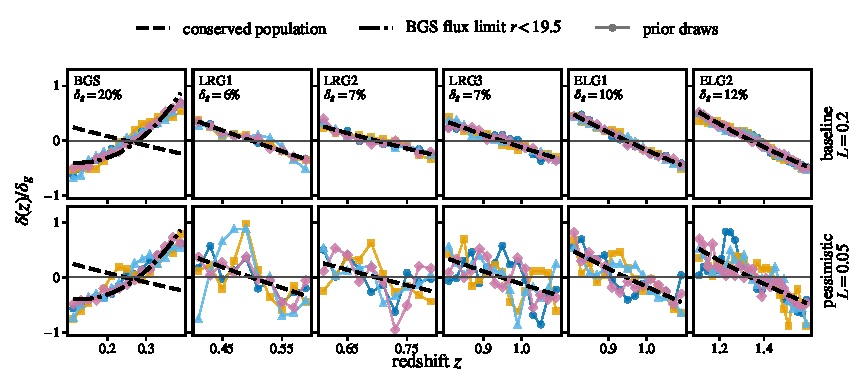
\includegraphics[width=\linewidth]{plots/prior_draws/prior_draws.pdf}
  \caption{Draws of the two stated priors on the $\Delta z = 0.02$
    bins, one column per group: the baseline prior (top row;
    $\sigma_g = 3\%$ for BGS and $1\%$ elsewhere, $L = 0.2$) and the
    pessimistic prior (bottom row; $\sigma_g = 3\%$, $L = 0.05$).  Each
    column is divided by the round constant $\delta_g$ in its top panel,
    so all panels share one axis.  Thick dashed: the conserved-population
    drift; thick dash-dot (BGS): the $r < 19.5$ flux-limit drift.  Thin
    curves: four draws of $\delta(z)$, each on the line of the group's
    reference drift (the flux limit in BGS, the conserved population
    elsewhere), so draw and drift differ by the residual
    $\varepsilon$.}
  \label{fig:priordraws}
\end{figure}

\section{Model A}
\label{sec:modela}

Linear bias alone is not enough at this cut: in the companion note
\texttt{notes/linear\_bias\_kmax}, a linear-bias fit to a one-loop truth
at $\kmax = 0.075\hMpc$ moves $\Omega_m$ by $1.5$--$1.8\sigma$ and
$(w_0, w_a)$ by $0.28$--$0.55\sigma$ on the
$\Delta d_{\rm com} = 62$~Mpc layout under the four linear-bias priors,
and linear bias is safe only at $\kmax = 0.05\hMpc$.
Model A, of \texttt{notes/higher\_order\_bias}, keeps the per-bin
linear bias of Eq.~\eqref{eq:summodel} and adds the one-loop terms.  As
computed here, the real-space galaxy power spectrum of bin $i$ is
\begin{equation}
  P_{gg,i}(k) \;=\; b_{1,i}^2\,P_{\rm mm}(k)
  \;+\; P_{\rm loop}(k;\, b_{1,i}, b_{2,i}, b_{s^2,i})
  \;+\; \alpha_0\,k^2 P_{\rm mm}(k)
  \;+\; \frac{{\rm SN}_0}{\bar{n}_i} ,
  \label{eq:modela}
\end{equation}
where $P_{\rm mm}$ is the nonlinear matter power spectrum and
$P_{\rm loop}$ holds the one-loop terms.  These carry the quadratic
bias $b_2$, the response of the galaxy density to the square of the
matter density contrast $\delta_m$ (the galaxy density contrast
contains $b_2\,\delta_m^2/2$), and the tidal bias $\bstwo$, its
response to the squared tidal field; the third-order bias $b_3$ is
zero.  $\alpha_0$ is the $k^2$ counterterm, in $h^{-2}\,{\rm Mpc}^2$,
which absorbs the sensitivity of the loops to small scales.
${\rm SN}_0$ is the white-noise power beyond Poisson, in units of the
bin's Poisson power $1/\bar{n}_i$, with $\bar{n}_i$ the bin's number
density.  The higher-order biases follow each bin's own linear bias
through calibrations, plus one offset per group:
\begin{equation}
  b_{2,i} \;=\; b_2^{\rm L}(b_{1,i}) + \Delta_{2,g},
  \qquad
  b_{s^2,i} \;=\; -\tfrac{4}{7}\,(b_{1,i} - 1) + \Delta_{s,g},
  \label{eq:calibrations}
\end{equation}
with $b_2^{\rm L}$ the separate-universe fit of Lazeyras et
al.~\cite{Lazeyras2016} and the second relation the co-evolution of a
population formed with local bias~\cite{Saito2014}.

The priors are Gaussian and centered on zero: widths $1$ on
$\Delta_2$, $0.5$ on $\Delta_s$, $2$ on ${\rm SN}_0$ and
$0.5/\kmax^2 = 88.9\aunit$ on $\alpha_0$.  The $\alpha_0$ width is the
rule of the DESI 2024 full-shape analysis~\cite{DESI2024V,Maus2024}
moved to this cut: $\alpha_0 k^2 = 0.5$ at $k = \kmax$, a $50\%$
correction relative to $P_{\rm mm}$ at the $z = 0$ cut.  At bin $i$'s
own cut, $\kmax/D(\bar{z}_i)$, the same width gives
$\alpha_0 k^2 = 0.5/D(\bar{z}_i)^2$.  Relative to the linear galaxy
power $b_{1,i}^2 P_{\rm mm}$ both are smaller by a further factor
$b_{1,i}^2$.  Redshift-space distortions are linear (Kaiser), with
each bin's redshift distribution convolved by the sampled velocity
dispersion $\sigma_v$ (the Fingers-of-God smearing), as in the
linear-bias run.

Two variants of the higher-order sector sit on every linear-bias prior.
\textbf{Model A baseline} has one $\Delta_2$, $\Delta_s$, $\alpha_0$
and ${\rm SN}_0$ per group, $24$ parameters.  \textbf{Model A
pessimistic} also tilts the $\Delta_2$, $\Delta_s$ and $\alpha_0$ of
each group linearly in redshift, with flat priors on the tilts, up to
$42$ parameters.  ${\rm SN}_0$ is not tilted, by choice: its Poisson
part is known bin by bin, and the excess is kept at one number per
group.  Appendix~\ref{app:impl} describes the implementation and the
Fisher matrices.

\section{The accuracy test}
\label{sec:accuracy}

No mock catalogs and only two derived drift laws are available, so
this note does not defend one prior.  It tests each prior against
random truths and quotes the FoM only for the priors that pass.

\paragraph{Random truths.}
Each truth sets every bin's linear bias to its group's known drift
(the $r < 19.5$ flux limit in BGS, a conserved galaxy population
elsewhere; Appendix~\ref{sec:driftlaws}) plus a residual drawn from
the baseline or the pessimistic prior, $2000$ truths per family
(Appendix~\ref{sec:randomtruths}).  The truth's $b_2$ and $\bstwo$
follow its $b_1$ through Eq.~\eqref{eq:calibrations}.  Every
linear-bias prior fits every truth under both variants, centered on the
growth-tied shape, to first order in the truth
(Appendix~\ref{sec:biasformula}).  Figure~\ref{fig:scatter} draws the
$(w_0, w_a)$ shift of each fit in units of its own ellipse, without
data noise.  Where a fit's prior equals the truth's scatter, the mean
shift is not a bias: that fit's ellipse already includes this scatter
(Appendix~\ref{sec:inflation}).

\begin{figure}[tbp]
  \centering
  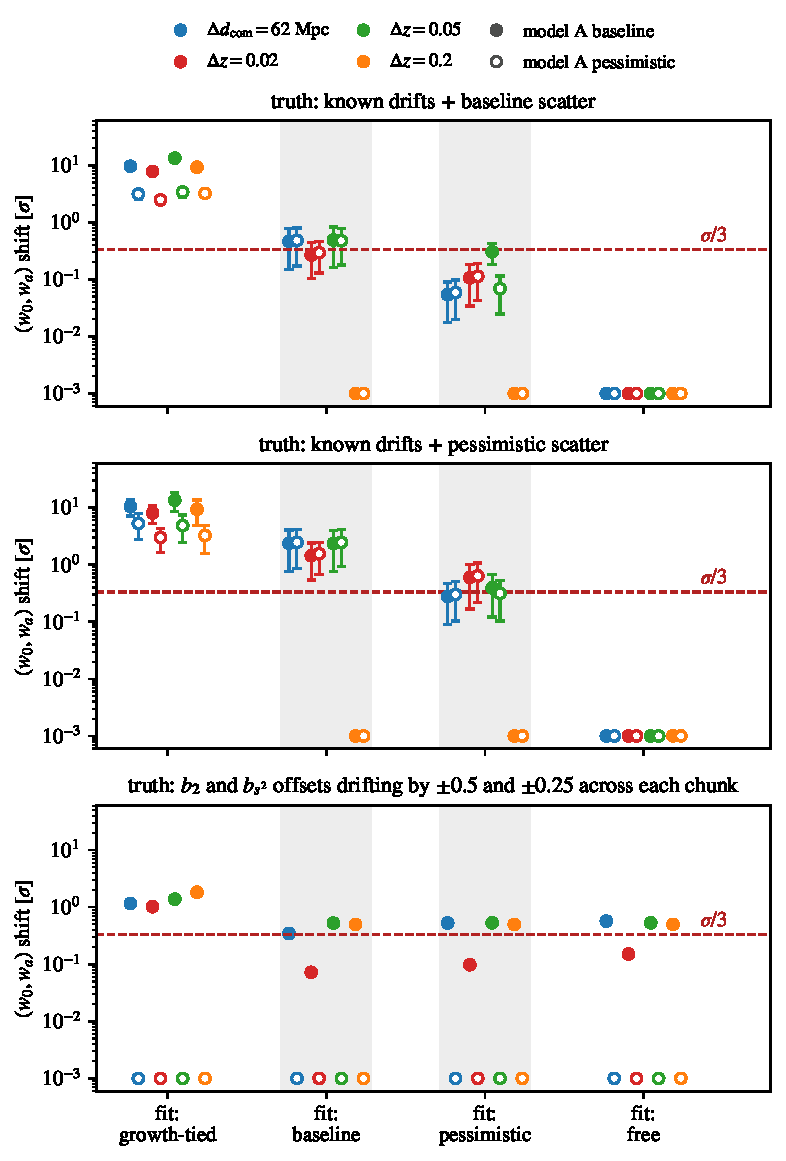
\includegraphics[width=0.62\linewidth]{plots/ladder_bias_scatter/ladder_bias_scatter.pdf}
  \caption{The $(w_0, w_a)$ shift of each fit in units of its own
    marginalized ellipse, under model A, for $2000$ truths: the known
    drifts plus a residual drawn from the baseline prior (top) or the
    pessimistic prior (bottom), without data noise.  Filled: model A
    baseline; open: model A pessimistic; colors: the layouts.  Points:
    the mean shift; bars: the 16th--84th percentiles.  Gray columns: the
    baseline and pessimistic priors.  Dashed line: $\sigma/3$.  Points
    at $10^{-3}$: exact zeros.  \kmaxclause}
  \label{fig:scatter}
\end{figure}

\paragraph{The statistic.}
Each fit is scored by
\begin{equation}
  \chidof ,
  \qquad
  \chi^2 = \Delta p\T\, \mathsf{C}_p^{-1}\, \Delta p ,
  \label{eq:gof}
\end{equation}
with $\Delta p$ the recovered minus the true parameters,
$\mathsf{C}_p$ the fit's marginalized covariance, $n_{\rm dof} = 2$ for
$p = (w_0, w_a)$ and $1$ for $\Omega_m$ or $A_s$, and
$\langle\cdot\rangle$ the exact average over the data noise and the
bias history (the known drift plus a random residual).  Its value,
written $\eta$, is $1$ for error bars that cover the truth as often as
they claim; above $1$ they are too small, and below $1$ conservative.
It scores the recovery of the parameters, not the $\chi^2$ of the
data: a biased fit can match the band powers while its cosmology is
wrong.  Appendix~\ref{app:bias} derives it and converts it into the
fraction of universes in which a one-parameter $1\sigma$ bar covers the
truth; the percentages below come from that conversion.

\begin{figure}[tbp]
  \centering
  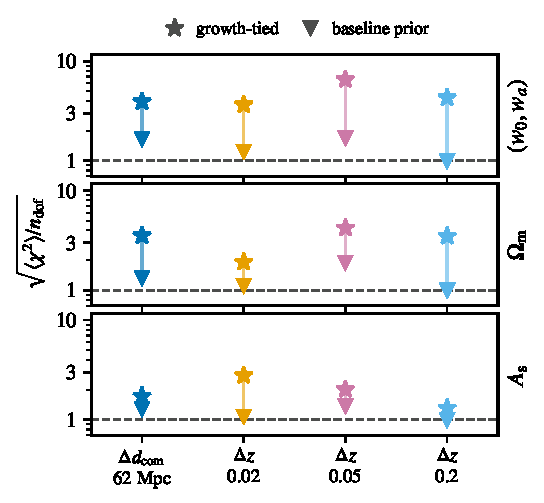
\includegraphics[width=0.62\linewidth]{plots/goodness_of_fit/goodness_of_fit.pdf}
  \caption{How well each fit's quoted error bar covers where the fit
    actually lands, measured by $\eta = \chidof$:
    $\chi^2 = \Delta p\T \mathsf{C}_p^{-1} \Delta p$, with $\Delta p$
    the recovered minus the true parameters and $\mathsf{C}_p$ the
    fit's marginalized covariance; $n_{\rm dof} = 2$ for $(w_0, w_a)$,
    $1$ for $\Omega_m$ or $A_s$; $\langle\cdot\rangle$ averages over the
    data noise and the bias history (the known drifts plus a residual
    from the pessimistic prior).  For one parameter, the $1\sigma$ bar
    covers the truth in a fraction $2\Phi(1/\eta) - 1$ of the universes
    ($\Phi$ the Gaussian cumulative distribution): $68\%$ at $\eta = 1$
    (dashed line), $38\%$ at $\eta = 2$.  Model A baseline; squares:
    the growth-tied prior; circles: the baseline prior.  Omitted: the
    free prior (exactly $1$) and the pessimistic prior (at most
    $1.05$).  \kmaxclause}
  \label{fig:gof}
\end{figure}

\paragraph{The result of the test.}
Figures~\ref{fig:scatter} and \ref{fig:gof} order the priors.
\begin{itemize}
  \item \emph{The growth-tied prior fails under every truth and is
    discarded.}  The conserved-population drift alone moves its
    $(w_0, w_a)$ by several $\sigma$ (Appendix~\ref{sec:tabdrifts}),
    and its error bars are far too small under both scatters; under the
    pessimistic scatter its $\Omega_m$ bar covers the truth in only
    $5$--$39\%$ of universes.
    Under model A pessimistic, whose flat-prior tilts follow part of a
    linear-bias drift, $\eta$ falls to $1.4$--$2.3$ in $(w_0, w_a)$,
    still far from honest.  A prior whose error bars do not cover the
    truth has no meaningful FoM.
  \item \emph{The baseline prior is honest only if the bias residual is
    as smooth as it assumes.}  Under its own scatter $\eta$ is
    $1.00$--$1.02$.  Under the pessimistic scatter it fails on every
    layout but $\Delta z = 0.2$ (Section~\ref{sec:prior}): the $\Omega_m$ bar
    covers the truth in only $56$, $63$ and $40\%$ of universes on
    $\Delta d_{\rm com} = 62$~Mpc, $\Delta z = 0.02$ and $0.05$, and the
    $A_s$ bar in $57$, $65$ and $54\%$.  Because the noise term of
    $\langle\chi^2\rangle$ is at most one, the rms displacement beyond
    the noise is at least $(\eta^2 - 1)^{1/2}$ error bars
    (Appendix~\ref{sec:inflation}).  Model A pessimistic does not change
    this.
  \item \emph{The pessimistic prior is honest under both scatters}:
    $\eta \le 1.05$ in every score, and $0.89$--$1.00$ in $(w_0, w_a)$
    (conservative) under baseline scatter.  The $1.05$ comes from the BGS
    flux-limit drift on $\Delta z = 0.05$, which this prior leaves just
    above $\sigma/3$ (Appendix~\ref{sec:tabdrifts}).  The free prior
    gives exactly $1$.
\end{itemize}

\paragraph{A drift of the calibrations.}
The random truths move only the linear bias; the higher-order biases
follow it through calibrations assumed exact up to one constant offset
per group.  A third truth tests that assumption.  It drifts the offsets
linearly with the bin redshift across each group, $\Delta_2$ from
about $-0.5$ to $+0.5$ and $\Delta_s$ from about $-0.25$ to $+0.25$
(half the prior width at each end), and keeps $b_1$ at its fiducial
(Appendix~\ref{sec:ladderimpl}).  Under model A baseline
(Figure~\ref{fig:caldrift}) the shift of $(w_0, w_a)$ exceeds
$\sigma/3$ under every prior on the two wide layouts, $\Delta z = 0.05$
and $0.2$, and the $A_s$ shift of the baseline, pessimistic and free
priors reaches $\sigma/3$ on $\Delta z = 0.05$.
On the two thin layouts only the growth-tied prior exceeds $\sigma/3$.
Model A pessimistic absorbs this drift exactly, by construction: its
tilts have the drift's shape.  The test shows only that the tilts work
for a linear drift; a nonlinear drift of the calibrations within a
group is untested.

\begin{figure}[tbp]
  \centering
  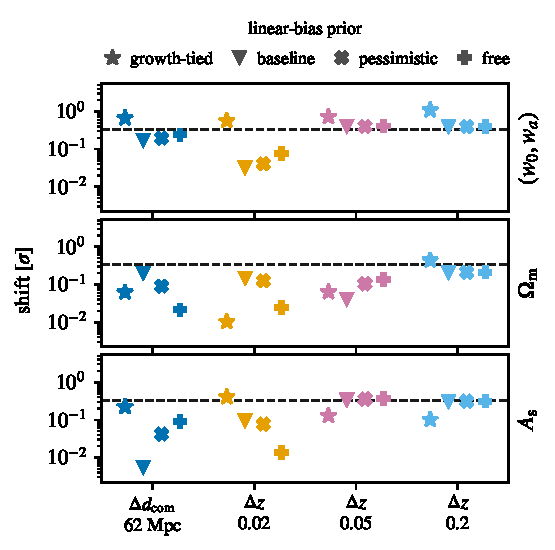
\includegraphics[width=0.62\linewidth]{plots/calibration_drift/calibration_drift.pdf}
  \caption{The shift of a model A baseline fit under the calibration
    drift ($\Delta_2$ and $\Delta_s$ changing linearly by $1$ and $0.5$
    across each group): $(w_0, w_a)$ in units of the fit's ellipse,
    $\Omega_m$ and $A_s$ in their own $\sigma$, per layout.  Markers:
    the four linear-bias priors.  Dashed line: $\sigma/3$.  Omitted:
    model A pessimistic, which absorbs the drift exactly by
    construction.  \kmaxclause}
  \label{fig:caldrift}
\end{figure}

\section{The figure of merit}
\label{sec:fom}

A FoM means something only for a prior that passes the accuracy test:
the pessimistic and free priors under both truths, the baseline prior
only if the bias residual is as smooth as it assumes.
Figure~\ref{fig:ladder} therefore draws these three priors, with
${\rm FoM}(w_0, w_a)$ in panel (a) and
${\rm FoM}(\Omega_m, 10^9 A_s)$ in panel (b), both from the same Fisher
inverse.  Both fall from the baseline prior to free under each
variant, except on $\Delta z = 0.2$, where the three priors coincide.
The two thin layouts carry most of the information.  Model A
pessimistic costs little against model A baseline on the thin layouts
and more on the wide ones.  DESI $C_\ell^{gg}$ alone sits well below
LSST Y1 3x2pt~\cite{DESCSRD2018} in both figures of merit at this cut.
Appendix~\ref{app:comparison} sets these FoMs next to the linear-bias
run and to exact calibrations, neither of which is a result here.

\begin{figure}[tbp]
  \centering
  \begin{minipage}[b]{0.49\linewidth}
    \centering
    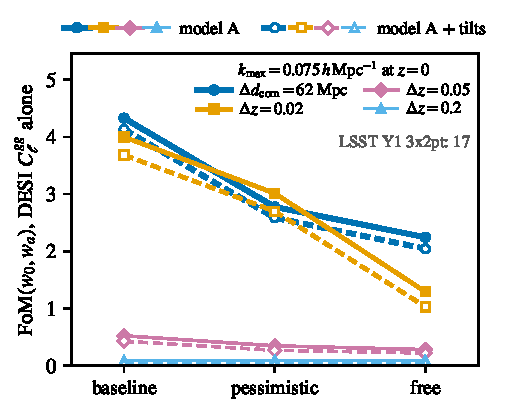
\includegraphics[width=\linewidth]{plots/baseline_ladder/baseline_ladder.pdf}\\[0.2em]
    {\small (a)}
  \end{minipage}\hfill
  \begin{minipage}[b]{0.49\linewidth}
    \centering
    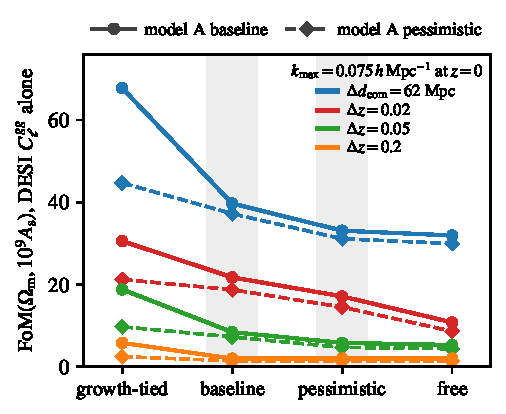
\includegraphics[width=\linewidth]{plots/baseline_ladder/baseline_ladder_om_as.pdf}\\[0.2em]
    {\small (b)}
  \end{minipage}
  \caption{\textbf{(a)} ${\rm FoM}(w_0, w_a)$ and \textbf{(b)}
    ${\rm FoM}(\Omega_m, 10^9 A_s)$ of DESI $C_\ell^{gg}$ alone under the
    baseline, pessimistic and free priors.  Colors: the bin layouts.
    Solid: model A baseline; dashed: model A pessimistic.  The text in
    each panel quotes the LSST Y1 3x2pt value of the same figure of
    merit, which lies far above the DESI points.  \kmaxclause}
  \label{fig:ladder}
\end{figure}

\paragraph{Result.}
The headline is model A pessimistic on the pessimistic prior: it is
honest under both families of random truths and absorbs a linear
calibration drift exactly.  Model A baseline on the baseline prior
shows what better knowledge of bias evolution would buy.  It holds
only under two assumptions: each bin's linear-bias residual is no
larger and no rougher than the baseline prior, and the calibrations of
$b_2$ and $\bstwo$ hold within a group up to one constant offset.  If
the first fails at the pessimistic size, the $\Omega_m$ bar covers the
truth in only $40$--$63\%$ of universes; if the second fails by the
linear drift above, $(w_0, w_a)$ moves by more than $\sigma/3$ on the
wide layouts.  The free prior under model A pessimistic is the lower
limit, and the growth-tied prior is discarded.

\clearpage

\appendix

% Physics appendices of correlated_bias_prior_v2.tex, read with
% % Physics appendices of correlated_bias_prior_v2.tex, read with
% % Physics appendices of correlated_bias_prior_v2.tex, read with
% \input{appendix_physics} right after \appendix.  No preamble: the
% macros \ones, \Prec, \Cov and \T come from the main file.  The labels
% are shared with the mathematics appendices (appendix_math.tex).

\section{The models}
\label{sec:models}

This appendix first builds the prior without the tilt of
Eq.~\eqref{eq:summodel}: the kernel model, in which the exponential
kernel describes the whole deviation $\delta_i$ of a bin from its
group's trend.  Appendix~\ref{sec:memory} adds the free tilt, and the
kernel then describes the residual $\varepsilon_i$ around each group's
line.  In the appendices $b_i$ is the linear bias $b_{1,i}$ of bin $i$.

\subsection{Growth-tied, free, and correlated biases}
\label{sec:defs}

The growth-tied model sets $b_i = B_g/D(\bar{z}_i)$, with one free
amplitude $B_g$ per group.  The kernel model multiplies it by a
fractional deviation $\delta_i$,
\begin{align}
  b_i &\;=\; \frac{B_g}{D(\bar{z}_i)}\,\bigl(1 + \delta_i\bigr),
  \label{eq:model}
  \\
  \bigl\langle \delta_i\,\delta_j \bigr\rangle
  &\;=\; \sigma_g^2\,
  \exp\!\left(-\,\frac{|\bar{z}_i - \bar{z}_j|}{L}\right),
  \label{eq:priorkernel}
\end{align}
with $B_g$ still free (flat prior) and the prior zero across groups.
In the Fisher matrix the convenient parameters are the per-bin
amplitudes
\begin{equation}
  \beta_i \;\equiv\; B_g\,\bigl(1 + \delta_i\bigr),
  \qquad \text{fiducial } \beta_i = B_g,
  \label{eq:beta}
\end{equation}
so that $b_i = \beta_i / D(\bar{z}_i)$.  Since
$\beta_i - B_g = B_g\,\delta_i$, the prior covariance of the $\beta_i$
within one group is
\begin{equation}
  \Cov \;=\; \sigma_\beta^2\,\mathsf{R},
  \qquad
  \sigma_\beta \;=\; \sigma_g\,B_g,
  \qquad
  \mathsf{R}_{ij} \;=\; \exp\!\left(-\,\frac{|\bar{z}_i - \bar{z}_j|}{L}\right),
  \label{eq:covdef}
\end{equation}
with $\sigma_\beta$ the spread of one amplitude, in units of a bias, and
$\mathsf{R}$ the dimensionless correlation matrix.

\subsection{What $\sigma_g$ and $L$ mean}
\label{sec:jump}

The diagonal of the kernel gives the wander of a single bin,
$\mathrm{Var}(\delta_i) = \sigma_g^2$.  The correlation coefficient of
two bins at separation $\Delta z = |\bar{z}_i - \bar{z}_j|$ is
\begin{equation}
  r \;=\;
  \frac{\langle \delta_i \delta_j \rangle}
       {\sqrt{\langle \delta_i^2 \rangle\,\langle \delta_j^2 \rangle}}
  \;=\; e^{-\Delta z / L} ,
  \label{eq:rdef}
\end{equation}
set by the separation and $L$ alone.  The jump between the two bins has
variance
\begin{equation}
  \mathrm{Var}(\delta_i - \delta_j)
  \;=\;
  2\,\sigma_g^2\left(1 - e^{-\Delta z / L}\right)
  \;\approx\;
  \frac{2\,\sigma_g^2\,\Delta z}{L}
  \quad (\Delta z \ll L).
  \label{eq:jumpvar}
\end{equation}
At small separations the jump variance grows linearly with
$\Delta z$, as for a random walk; only beyond $L$ does the finite
wander pull the deviation back.  For neighbors at $\Delta z = 0.02$
with $L = 0.05$, $r = e^{-0.4} = 0.670$ and the exact rms jump is
$0.81\,\sigma_g$; the small-separation form gives $0.89\,\sigma_g$,
because $\Delta z/L = 0.4$ is not small.

\subsection{The free group amplitude and the projection}
\label{sec:projintro}

A plain Gaussian prior with covariance $\Cov$ would charge for moving
all $\beta_i$ of a group together, but that uniform shift is the free
amplitude $B_g$.  The repair removes the uniform direction: with
$\ones$ the ones vector of the group's $n$ bins, the prior precision
of a group's amplitudes is
\begin{equation}
  \Prec \;=\; \Cov^{-1}
  \;-\;
  \frac{\Cov^{-1}\ones\,\ones\T \Cov^{-1}}{\ones\T \Cov^{-1} \ones}.
  \label{eq:projdef}
\end{equation}
$\Prec\,\ones = 0$, so a uniform shift costs nothing; a pure shape
change keeps the penalty of the plain prior; $\Prec$ is positive
semidefinite (no displacement has a negative penalty) with rank
$n - 1$; and $\Prec$ is exactly the prior
obtained by sampling $B_g$ with a flat prior and marginalizing it.
Appendices~\ref{sec:twobins}, \ref{sec:threeviews} and
\ref{sec:general} show these for two bins, by marginalization, and for
$n$ bins.  Across groups the prior is zero, so the full prior
precision is block diagonal.

\section{Which $L$ and $\sigma_g$ are physical}
\label{sec:physical}

One case of bias evolution can be solved in closed form: a population
whose members are conserved.  This appendix derives it, measures its
deviation from the growth-tied trend, lists what breaks conservation in
a selected sample, and weighs the published measurements.

\subsection{A conserved population: the bias continuity equation}
\label{sec:conserved}

Take a sample whose membership never changes, with no velocity bias,
in linear theory.  The matter overdensity $\delta_m$ and the
galaxy-count overdensity $\delta_{\rm gal}$ then obey the same
continuity equation with the same velocity field, so the excess
clumping $\delta_{\rm gal} - \delta_m$ is frozen
(Appendix~\ref{app:continuity}).  With $b_c$ the linear bias at a
reference redshift $z_c$ and $\delta_m \propto D$, the frozen
difference gives~\cite{Fry1996}
\begin{equation}
  b(z) - 1
  \;=\;
  \bigl(b_c - 1\bigr)\,\frac{D(z_c)}{D(z)} :
  \label{eq:fry}
\end{equation}
the excess set at formation stays fixed while the matter clustering
grows, so the bias decays toward one.  The growth-tied shape freezes a
different quantity: constant $b\,D$ means a galaxy clustering amplitude
$b\,\delta_m$ that does not grow, which describes a selection that
picks, at each redshift, a different and rarer set of objects.

\subsection{The deviation from the growth-tied trend}
\label{sec:tilt}

Place the reference at a group's midpoint $z_c$, with
$b_c = B/D(z_c)$.  The ratio of Eq.~\eqref{eq:fry} to the growth-tied
bias $b_c\,D(z_c)/D(z)$ gives the deviation of Eq.~\eqref{eq:model},
\begin{equation}
  \delta(z)
  \;=\;
  \frac{D(z)/D(z_c) - 1}{b_c} ,
  \label{eq:tilt}
\end{equation}
zero at the midpoint, positive at lower redshift and negative at higher
redshift, and nearly linear across a group because $D$ is smooth.  In
flat $\Lambda$CDM with $\Omega_m = 0.3$ and the project's fiducial
amplitudes it is $+5.3\%$ and $-4.9\%$ at the ends of BGS ($B = 1.34$,
$0.1 < z < 0.4$, $b_c = 1.5$), $+2.4\%$ and $-2.2\%$ at the ends of LRG1
($B = 1.70$, $0.4 < z < 0.6$, $b_c = 2.2$), and $+2.6\%$ and $-2.3\%$ at
the ends of LRG3 ($B = 1.70$, $0.8 < z < 1.1$, $b_c = 2.7$).  Between
neighbors it changes by $0.3$--$0.7\%$ at $\Delta z = 0.02$ and
$0.8$--$1.7\%$ at $\Delta z = 0.05$: a smooth tilt, coherent over the
whole group.  For comparison, the neighbor rms of
Eq.~\eqref{eq:jumpvar} at $\Delta z = 0.02$ (and $0.05$) is $2.4\%$
($3.4\%$) for $\sigma_g = 3\%$ and $L = 0.05$, and $0.44\%$ ($0.67\%$)
for $\sigma_g = 1\%$ and $L = 0.2$.  Figure~\ref{fig:theorybz} draws
these shapes: the conserved curve is flatter than $B_g/D$ in every
group, while the BGS flux-limit curve is much steeper, and convex.

\begin{figure}[htbp]
  \centering
  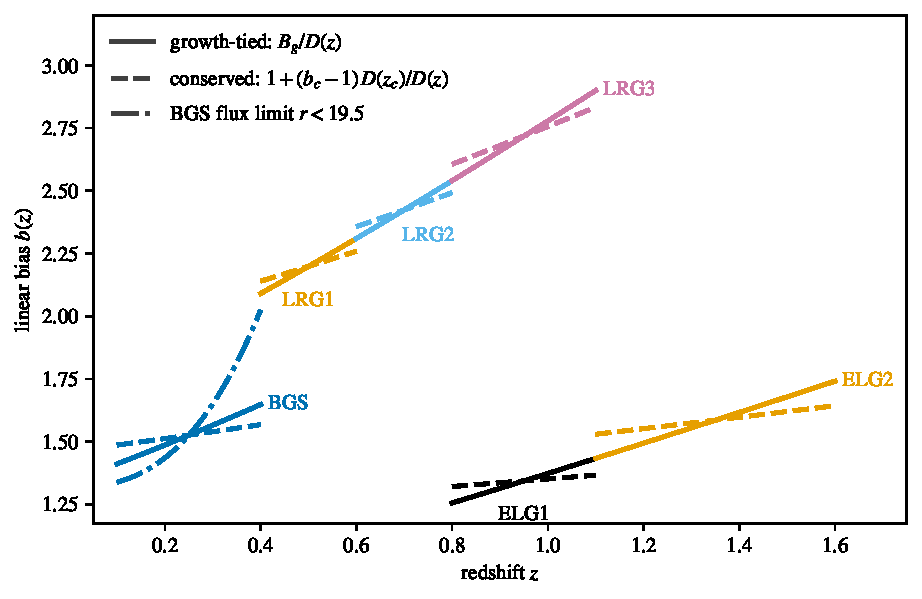
\includegraphics[width=\linewidth]{plots/theory_bz/theory_bz.pdf}
  \caption{The bias $b(z)$ of every group.  Solid: the growth-tied
    shape $B_g/D(z)$.  Dashed: a conserved population anchored at the
    group midpoint (Eq.~\eqref{eq:fry}).  Dash-dot, on BGS only: the
    $r < 19.5$ flux-limit bias, anchored at the same midpoint.}
  \label{fig:theorybz}
\end{figure}

\subsection{What breaks conservation in a selected sample}
\label{sec:selection}

\begin{itemize}
  \item \textbf{Threshold drift.}  A selection holds a roughly constant
    comoving density until the flux limit bites; beyond, it keeps only
    its brighter, more biased members.  The change is smooth, with $L$
    comparable to the group width.
  \item \textbf{Color-selection features.}  A spectral feature crossing
    a filter edge moves a color cut quickly in redshift.  The sharpest
    is the $4000$~\AA\ break, the step in an old galaxy's rest-frame
    spectrum at $4000$~\AA, which redshift slides across the filters: a
    filter edge $100$--$200$~\AA\ wide maps to
    $\Delta z = \Delta\lambda/(4000~\text{\AA}) \approx 0.03$--$0.05$.  The crossing is known; its
    amplitude in bias is unmeasured.
  \item \textbf{Mergers} turn two members into one.
  \item \textbf{Emission-line selection.}  An ELG belongs to the sample
    while its lines are strong, so membership follows the
    star-formation phase.
\end{itemize}

\subsection{What the measurements say}
\label{sec:evidence}

Each statement is tagged \emph{measured} (read from the cited source),
\emph{derived} (computed here from measured inputs) or \emph{assumed}.
Equation~\eqref{eq:fry} is from Fry~\cite{Fry1996};
Tegmark and Peebles~\cite{TegmarkPeebles1998} rederive it.

\paragraph{Massive red galaxies follow the conserved shape.}
SDSS and 2SLAQ LRGs at $0.19 < z < 0.55$, matched in color and
luminosity, show no significant evolution of the clustering amplitude
and merge at $7.5 \pm 2.3\%$ over that range, about $2.4\%$ per
Gyr~\cite{Wake2008} (measured).  The BOSS progenitors of the SDSS LRGs
merge at $2 \pm 1.5\%$ per Gyr and cluster as the continuity equation
predicts~\cite{Tojeiro2012}, and CMASS samples of fixed comoving
density at $0.43 < z < 0.7$ cluster like a conserved
population~\cite{Guo2013} (measured).  The bias of DESI-like LRGs in
photometric bins of $\Delta z \approx 0.1$ stays within $\pm 2.3\%$ of
$b = 1.5/D$ below $z = 0.83$, with the highest bin $6.4 \pm 6.4\%$
high~\cite{Zhou2021} (measured biases, residuals derived;
Figure~\ref{fig:zhou}).

\begin{figure}[htbp]
  \centering
  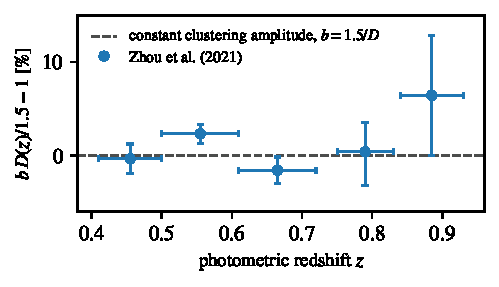
\includegraphics{plots/zhou_lrg_bias/zhou_lrg_bias.pdf}
  \caption{The measured bias of DESI-like LRGs~\cite{Zhou2021} as a
    fractional residual around $b = 1.5/D$, with $D$ at each
    photometric bin's center (flat $\Lambda$CDM, $\Omega_m = 0.3$);
    horizontal bars: the bin edges.}
  \label{fig:zhou}
\end{figure}

\paragraph{The selections drift.}
The DESI LRG cuts hold the comoving density near
$5 \times 10^{-4}\,(h/{\rm Mpc})^3$ at $0.4 < z < 0.8$ and hand over to
a fixed flux limit beyond~\cite{Zhou2023lrg} (measured).  That limit
raises the luminosity threshold by $0.27$ magnitudes per
$\Delta z = 0.1$ at $z \approx 1$; times the threshold-bias slope of
SDSS luminosity-threshold samples, $b\,(\sigma_8/0.8) = 1.06 +
0.21\,(L_{\rm th}/L_*)^{1.12}$~\cite{Zehavi2011} ($0.5$--$1.0$ in bias
per magnitude near LRG luminosities; measured), it drifts the LRG3 bias
by $6$--$11\%$ per $\Delta z = 0.1$ on top of $B/D$ (derived, from an
$r$-band relation outside its calibrated range, so only the direction
and order of magnitude hold).  BGS Bright is magnitude limited at
$r < 19.5$~\cite{Hahn2023} (measured), which drives a $10$--$25\%$ bias
drift across the group (derived; Appendix~\ref{app:bgsflux}).

\paragraph{The ELG bias shape is stable.}
Fits of the halo occupation distribution (HOD: how many sample
galaxies live in a halo of each mass) to the DESI One-Percent ELGs in
$0.8 < z < 1.1$ and
$1.1 < z < 1.6$ agree within one sigma~\cite{Rocher2023} (measured);
at these host masses the halo bias depends weakly on mass, so the
implied drift is at the percent level (derived, slope assumed).  The
[OII] doublet loses signal-to-noise in windows
$\Delta z \approx 0.001$--$0.01$ wide where it lands on sky lines,
especially at $z > 1.5$~\cite{Raichoor2023} (measured): the one
short-separation mechanism with a measured location, with an assumed
bias amplitude of $1$--$2\%$.

\paragraph{Nothing resolves bias below $\Delta z \approx 0.1$.}
The CMB-lensing tomography of the same samples~\cite{White2022,
Sailer2024, Sailer2025}, on the photometric samples of
Zhou et al.~\cite{Zhou2023tomo}, uses bins of about $0.15$ with one
free bias per bin and finds smooth models that fit.  Below
$\Delta z \approx 0.1$ this note rests on the continuity equation and
the selection arguments.

\section{The memory model}
\label{sec:memory}

\subsection{Why a second model}
\label{sec:memwhy}

Every deviation above except the sky-line windows is a monotonic drift:
the conserved-population tilt (about $1\%$ per $\Delta z = 0.05$), the
LRG3 magnitude-limit drift ($6$--$11\%$ per $\Delta z = 0.1$) and the
BGS flux-limit drift ($10$--$25\%$ across the group).  The kernel model
admits such a drift only at a price: to pass a $20\%$ drift with
$L \leq 0.1$ it takes $\sigma_g = 10$--$15\%$, which also allows about
$10\%$ scatter between neighbors that no identified mechanism
produces.  One $\sigma_g$ controls both, so the kernel cannot say
``large smooth drift, small local scatter''.  The memory model
separates the two.

\subsection{Why the kernel forgets}
\label{sec:memforget}

At $L = 0.05$, bins $0.15$ apart share $e^{-3} \approx 0.05$ of their
deviation.  With $r_k = e^{-(\bar{z}_{k+1} - \bar{z}_k)/L}$ the
correlation of neighbors $k$ and $k+1$, the best guess of the next bin
given all earlier ones is (Appendix~\ref{app:chain})
\begin{equation}
  \mathrm{E}\bigl[\delta_{k+1} \mid \delta_1, \dots, \delta_k\bigr]
  \;=\; r_k\, \delta_k :
  \label{eq:memmarkov}
\end{equation}
only the nearest neighbor matters, and the influence of any one bin
fades along the chain.

\subsection{The model, and why it remembers}
\label{sec:memmodel}

The memory model adds a tilt per group and splits the deviation into a
line and a residual,
\begin{equation}
  \delta_i \;=\; s_g\, v_i + \varepsilon_i,
  \qquad
  v_i \;=\; \bar{z}_i - \bar{z}_g,
  \label{eq:memdef}
\end{equation}
with $s_g$ a free tilt (flat prior, like $B_g$) and $\varepsilon_i$
carrying the kernel of Eq.~\eqref{eq:priorkernel}: the model of
Eqs.~\eqref{eq:summodel} and \eqref{eq:sumkernel}.  Giving the slope a
Gaussian prior of variance $\tau^2$ first (the flat prior is
$\tau \to \infty$), the deviations have covariance
\begin{equation}
  \mathrm{Cov}(\delta_i, \delta_j)
  \;=\;
  \tau^2\, v_i\, v_j
  \;+\;
  \sigma_g^2\, e^{-|\bar{z}_i - \bar{z}_j|/L} .
  \label{eq:memcov}
\end{equation}
The new term does not decay with separation.  Far beyond $L$ the
correlation coefficient tends to
\begin{equation}
  \rho_{ij}
  \;\longrightarrow\;
  \frac{\tau^2 v_i v_j}
       {\sqrt{\bigl(\tau^2 v_i^2 + \sigma_g^2\bigr)
              \bigl(\tau^2 v_j^2 + \sigma_g^2\bigr)}}
  \;\longrightarrow\; \pm 1
  \quad \text{when } \tau |v| \gg \sigma_g :
  \label{eq:memrho}
\end{equation}
the two ends of a group remember each other through the shared slope.
The best guess of the next bin becomes
\begin{equation}
  \mathrm{E}\bigl[\delta_{k+1} \mid \delta_1, \dots, \delta_k\bigr]
  \;=\;
  \hat{c} + \hat{s}_g\, v_{k+1}
  \;+\;
  r_k\,\bigl(\delta_k - \hat{c} - \hat{s}_g\, v_k\bigr),
  \label{eq:memkriging}
\end{equation}
with $(\hat{c}, \hat{s}_g)$ the level and slope of the best straight
line through all past bins, weighted by $\Cov^{-1}$: every past bin
enters through the fitted line, and only the wiggle around it stays
Markov (the universal-kriging predictor; kriging is the geostatistics
name for the best linear prediction from correlated data;
Appendix~\ref{app:memory}).
Figure~\ref{fig:theorydraws} shows the difference on the BGS bins at
$\Delta z = 0.02$: kernel draws wide enough to admit the BGS drift
zigzag and forget, while memory draws are lines with small wiggles,
among which the drift looks typical.

\begin{figure}[htbp]
  \centering
  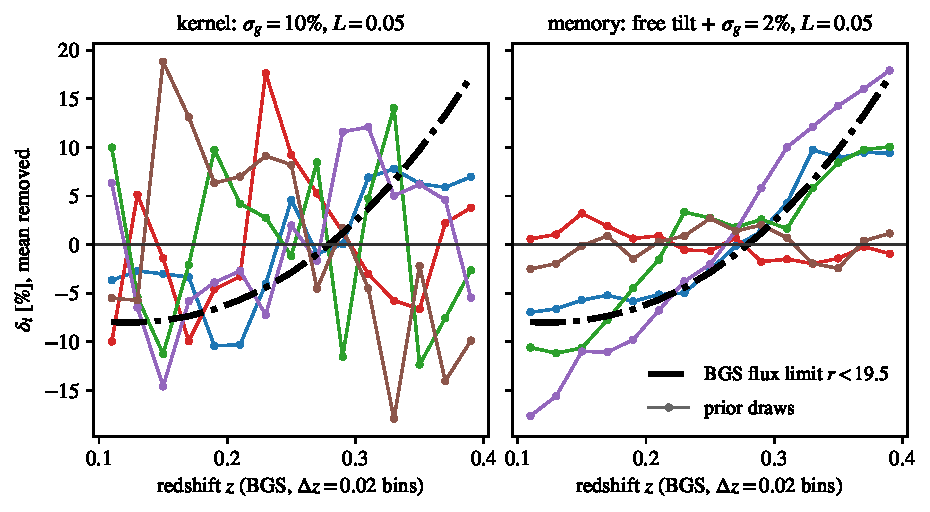
\includegraphics[width=\linewidth]{plots/theory_draws/theory_draws.pdf}
  \caption{Random prior draws of the deviations of the 15 BGS bins at
    $\Delta z = 0.02$, each draw's mean removed ($B_g$ is free).  Thick
    dash-dot: the BGS flux-limit drift.  Left: the kernel model.
    Right: the memory model, whose tilt is free in the model and drawn
    here, for display only, from a Gaussian of width $0.6$ per unit
    redshift.}
  \label{fig:theorydraws}
\end{figure}

\subsection{Why the memory model differs physically}
\label{sec:memphysics}

A selected sample changes along a group in two ways.  Coherent changes
move every bin the same way: a threshold that rises with distance, the
debiasing of a conserved population.  Local changes move bins
independently and are forgotten over a short range: the sky-line
windows and filter-edge crossings of Appendix~\ref{sec:selection}.  The
memory model gives the first kind to the tilt and the second to the
kernel.  One line suffices for the coherent kind, because the drifts
are smooth functions of $D(z)$ and the distance modulus.  The best
equal-weight line through each group's conserved deviation at the
$\Delta z = 0.05$ bin centers (derived; amplitudes $1.34$ for BGS,
$1.70$ for the LRGs and $0.84$ for the ELGs) removes deviations that
span $3$--$11\%$ and leaves $0.02$--$0.16\%$ rms, at most $0.27\%$
(ELG2).  The BGS flux-limit drift is larger and convex: it spans
$22.3\%$, and its best line leaves $2.4\%$ rms and $3.3\%$ at most
(Appendix~\ref{app:bgsflux}).  Figure~\ref{fig:theorydelta} shows both.
In the memory model $\sigma_g$ is the departure from the group's own
line, curvature plus local scatter: about $0.1\%$ for a conserved
population, $1$--$2\%$ for local selection features, $2$--$3\%$ for the
BGS curvature.

\begin{figure}[htbp]
  \centering
  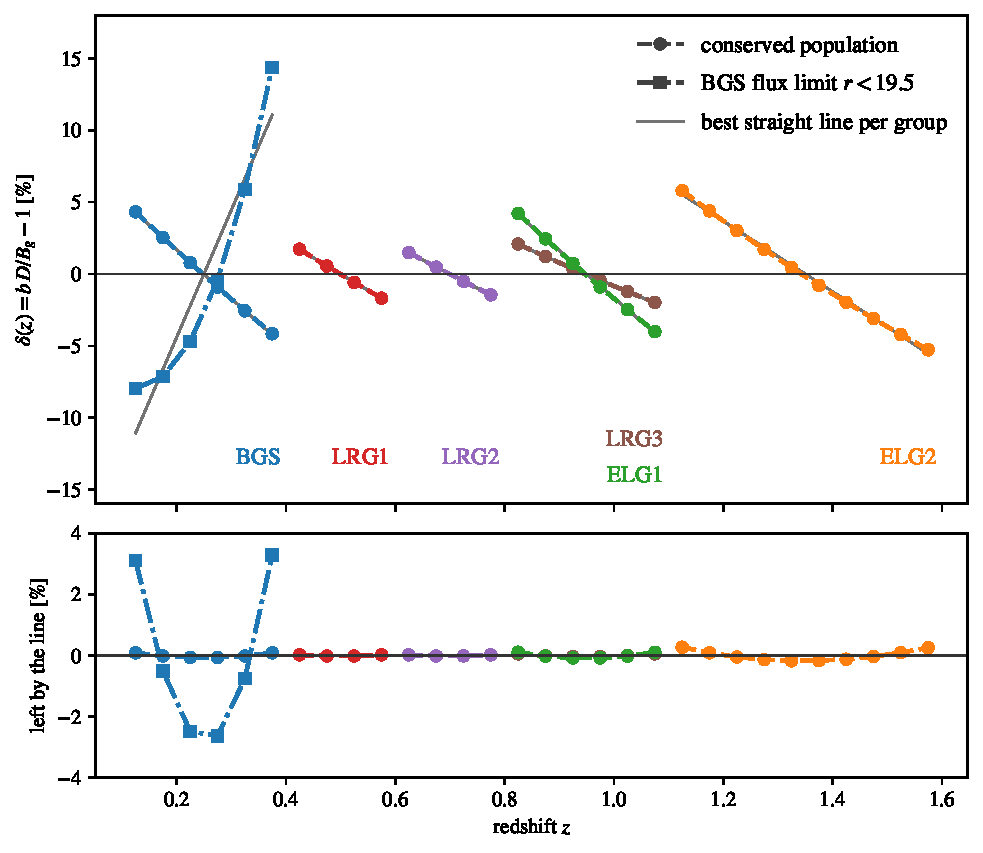
\includegraphics[width=\linewidth]{plots/theory_delta/theory_delta.pdf}
  \caption{Top: the deviation $\delta(z) = b\,D/B_g - 1$ at the
    $\Delta z = 0.05$ bin centers, with $B_g$ set so the mean deviation
    vanishes.  Dashed with circles: the conserved population, every
    group.  Dash-dot with squares: the BGS flux limit.  Thin gray: the
    best straight line per curve.  Bottom: what the line leaves.}
  \label{fig:theorydelta}
\end{figure}

\subsection{What the prior charges}
\label{sec:memcharge}

With flat priors on the line's level and slope, the prior precision of
a group's bin amplitudes is (Appendix~\ref{app:memory})
\begin{equation}
  \Prec_{\rm mem}
  \;=\;
  \mathsf{Q} - \mathsf{Q}\,\mathsf{U}
  \bigl(\mathsf{U}\T \mathsf{Q}\, \mathsf{U}\bigr)^{-1}
  \mathsf{U}\T \mathsf{Q},
  \qquad
  \mathsf{Q} = \Cov^{-1},
  \qquad
  \mathsf{U} = [\,\ones,\ v\,],
  \label{eq:memproj}
\end{equation}
the construction of Eq.~\eqref{eq:projdef} with one more column.  Its
penalty is
\begin{equation}
  \delta\T \Prec_{\rm mem}\, \delta
  \;=\;
  \min_{c,\, s_g}\;
  \bigl(\delta - c\,\ones - s_g\, v\bigr)\T
  \mathsf{Q}
  \bigl(\delta - c\,\ones - s_g\, v\bigr) :
  \label{eq:memmin}
\end{equation}
the prior subtracts the best straight line and charges only the
residual.  A monotonic drift of any size costs nothing; bumps around
the line still cost, and still forget over $L$.  $\mathsf{Q}$ is
tridiagonal (Appendix~\ref{sec:general}), while the subtracted term has
rank two and is dense, because the fitted line listens to every bin.
$\Prec_{\rm mem}\mathsf{U} = 0$, $\Prec_{\rm mem}$ is positive
semidefinite with rank $n - 2$, and a group of one or two bins has
$\Prec_{\rm mem} = 0$.

\section{The bias continuity equation, step by step}
\label{app:continuity}

The matter overdensity is $\delta_m = (\rho_m - \bar\rho_m)/\bar\rho_m$,
with $\bar\rho_m(t)$ the mean density; the galaxy-count overdensity
$\delta_{\rm gal}$ is defined the same way.  Conservation of mass and of
galaxy number gives, in comoving coordinates and to linear order (the
convective term $\mathbf{v} \cdot \nabla \delta$ is second order),
\begin{equation}
  \frac{\partial \delta_m}{\partial t}
  \;=\;
  -\,\frac{1}{a}\,\nabla \cdot \mathbf{v}_m,
  \qquad
  \frac{\partial \delta_{\rm gal}}{\partial t}
  \;=\;
  -\,\frac{1}{a}\,\nabla \cdot \mathbf{v}_{\rm gal},
  \label{eq:continuity}
\end{equation}
with $t$ cosmic time and $\mathbf{v}_m$, $\mathbf{v}_{\rm gal}$ the
peculiar velocities.  On large scales galaxies fall in the same
potential as the matter and carry no pressure of their own, so
$\mathbf{v}_{\rm gal} = \mathbf{v}_m$ (no velocity bias; galaxies as
test particles in Tegmark and Peebles~\cite{TegmarkPeebles1998}).
Subtracting the two equations and integrating from $z_c$,
\begin{equation}
  \delta_{\rm gal}(z) - \delta_m(z)
  \;=\;
  \delta_{\rm gal}(z_c) - \delta_m(z_c) :
  \label{eq:frozen}
\end{equation}
the excess clumping keeps its initial value.  With
$\delta_{\rm gal}(z_c) = b_c\,\delta_m(z_c)$ and
$\delta_m(z) = \delta_m(z_c)\, D(z)/D(z_c)$,
\begin{equation}
  \delta_{\rm gal}(z)
  \;=\;
  \delta_m(z)
  \left[\,1 + \bigl(b_c - 1\bigr)\,\frac{D(z_c)}{D(z)}\,\right],
  \label{eq:appsub}
\end{equation}
and dividing by $\delta_m(z)$ gives Eq.~\eqref{eq:fry}; dividing by the
growth-tied bias gives Eq.~\eqref{eq:tilt}.  As $D$ grows the frozen
term is divided by an ever larger number, so $b \to 1$: gravity
debiases a conserved sample.

Tegmark and Peebles also allow stochastic bias, with $b$ the ratio of
the galaxy to the matter fluctuation amplitude and $\rho_{gm}$ the
correlation coefficient of the two fields.  The same argument evolves
both: with $D$ normalized to one today and the subscript zero marking
today,
\begin{equation}
  b_0 =
  \left[(1 - D)^2 + 2 D (1 - D)\, b\, \rho_{gm}
  + D^2 b^2\right]^{1/2},
  \qquad
  \rho_{gm,0} = \frac{(1 - D) + D\, b\, \rho_{gm}}{b_0},
  \label{eq:tpevol}
\end{equation}
with $b$ and $\rho_{gm}$ the values at the epoch of growth factor $D$.
Both approach one as clustering grows, and for $\rho_{gm} = 1$
Eq.~\eqref{eq:tpevol} collapses to $b_0 - 1 = (b - 1)\,D$,
Eq.~\eqref{eq:fry} again.  For a DESI sample the assumption that
breaks is conservation (Appendix~\ref{sec:selection}); no velocity
bias and linear theory hold well on the scales kept.  The script of
Appendix~\ref{app:verify} integrates Eq.~\eqref{eq:continuity} and
recovers Eq.~\eqref{eq:fry} to $2 \times 10^{-9}$.

\section{The BGS flux-limit bias model, step by step}
\label{app:bgsflux}

This appendix derives the BGS drift of the baseline prior: a $22.3\%$
span, a convex shape, and a $2.4\%$ rms residual around the best line
(the function \texttt{bgs\_flux\_limit\_bias} of
\texttt{plots/make\_theory\_data.py}).

\subsection{The four steps}
\label{sec:bgssteps}

\paragraph{Step 1: the flux limit becomes a luminosity threshold.}
BGS Bright keeps every galaxy brighter than $r = 19.5$~\cite{Hahn2023}
($r$ the magnitude band).  The apparent magnitude $r$ and the absolute
magnitude $M$ are related by
$r = M + 25 + 5\log_{10}[d_L/(h^{-1}\,{\rm Mpc})] + K(z)$, with $d_L$
the luminosity distance and $K(z)$ the K-correction, the magnitude
correction for the part of the redshifted spectrum that falls outside
the observed band~\cite{BlantonRoweis2007}.  With $K = 0$ the faintest
absolute magnitude that passes at redshift $z$ is
\begin{equation}
  M_{\rm lim}(z) - 5\log_{10} h
  \;=\;
  19.5 - 25 - 5\log_{10} \frac{d_L(z)}{h^{-1}\,{\rm Mpc}},
  \qquad
  d_L(z) \;=\; (1+z)\,\chi(z),
  \label{eq:bgsmlim}
\end{equation}
with $\chi(z)$ the comoving distance of flat $\Lambda$CDM with
$\Omega_m = 0.3$ and $h$ the Hubble constant in units of
$100$~km/s/Mpc.

\paragraph{Steps 2 and 3: each bin is a threshold sample, and the
threshold sets the bias.}
At redshift $z$ the sample holds every galaxy with
$M < M_{\rm lim}(z)$, a threshold that brightens with distance.  The
SDSS luminosity-threshold samples at $z < 0.25$~\cite{Zehavi2011}
give
\begin{equation}
  b(>L_{\rm th})
  \;=\;
  1.06 + 0.21\,(L_{\rm th}/L_*)^{1.12},
  \qquad
  L_{\rm th}/L_* \;=\; 10^{-0.4\,(M_{\rm lim} - M_*)},
  \label{eq:bgszehavi}
\end{equation}
with $M_* - 5\log_{10} h = -20.44$ the characteristic magnitude of the
SDSS $r$-band luminosity function~\cite{Blanton2003}.  The model
applies the fit at every redshift, without evolution, and reads the
published $b\,(\sigma_8/0.8)$ as $b$.

\paragraph{Step 4: the deviation from the growth-tied shape.}
Because $B_g$ is free, only the shape of $b(z)$ matters; the amplitude
makes the mean deviation over the group's bin centers vanish:
\begin{equation}
  \delta(\bar{z}_i)
  \;=\;
  \frac{b(\bar{z}_i)\,D(\bar{z}_i)}{B} - 1,
  \qquad
  B \;=\; \frac{1}{n}\sum_{j=1}^{n} b(\bar{z}_j)\,D(\bar{z}_j).
  \label{eq:bgsdelta}
\end{equation}
At the six $\Delta z = 0.05$ bin centers of BGS, $z = 0.125$ to
$0.375$, the threshold brightens from $-18.56$ to $-21.24$, so
$L_{\rm th}/L_*$ grows from $0.18$ to $2.10$ and the bias from $1.09$
to $1.54$, while $D$ falls from $0.937$ to $0.824$.  The deviation runs
from $-8.0\%$ to $+14.4\%$, the $22.3\%$ span of
Figure~\ref{fig:theorydelta}.

\subsection{Why the drift is convex}
\label{sec:bgsconvex}

The bias rises by $41\%$ while $D$ falls by $12\%$, so the deviation
inherits the shape of the bias curve, which is flat at low redshift
and steep at high redshift: below $L_*$ the term
$0.21\,(L_{\rm th}/L_*)^{1.12}$ is small against $1.06$ ($0.03$ at the
first center), the threshold crosses $L_*$ near $z = 0.27$, and beyond
it the term rises exponentially ($0.48$ at the last center).  A
straight line through a convex curve leaves a U-shaped residual,
$(+3.1, -0.5, -2.5, -2.6, -0.8, +3.3)\%$ here.  Adding a quadratic term
cuts the residual from $2.4\%$ to $0.1\%$ rms, so the $2.4\%$ is the
curvature of the drift, the one part a free tilt cannot absorb.

\subsection{What the model leaves out}
\label{sec:bgsomissions}

None of the omissions changes the qualitative shape, a smooth,
monotonic, convex rise toward the far edge of the group.
\begin{itemize}
  \item \textbf{Evolution of the threshold-bias relation.}  The bias at
    fixed luminosity grows with redshift (Eq.~\eqref{eq:fry}), which
    steepens the drift; $M_*$ brightens by $1$--$2$ magnitudes per unit
    redshift~\cite{Blanton2003}, which flattens it, but only by
    $0.3$--$0.6$ magnitudes at the last center against the $2.68$ of
    the threshold.
  \item \textbf{No K-correction.}  A positive $K$, $0.37$ magnitudes at
    $z = 0.4$ for a spectrum flat in wavelength and more for a red
    one~\cite{BlantonRoweis2007}, makes the true threshold brighter at
    high redshift and steepens the drift.
  \item \textbf{Only $r < 19.5$.}  BGS Faint, at
    $19.5 < r < 20.175$~\cite{Hahn2023}, lowers the threshold by $0.675$
    magnitudes and flattens the drift; the fiber-magnitude cut and the
    color selection change the galaxy mix in a way
    Eq.~\eqref{eq:bgszehavi} cannot follow.
\end{itemize}
The model is an order-of-magnitude estimate, not a prediction of the
measured DESI BGS bias.  Its reliable content is the shape of the drift
and its size to a factor of order unity, which is what the baseline
prior uses: $\sigma_g = 3\%$ for BGS, from the $2$--$3\%$ curvature.
 right after \appendix.  No preamble: the
% macros \ones, \Prec, \Cov and \T come from the main file.  The labels
% are shared with the mathematics appendices (appendix_math.tex).

\section{The models}
\label{sec:models}

This appendix first builds the prior without the tilt of
Eq.~\eqref{eq:summodel}: the kernel model, in which the exponential
kernel describes the whole deviation $\delta_i$ of a bin from its
group's trend.  Appendix~\ref{sec:memory} adds the free tilt, and the
kernel then describes the residual $\varepsilon_i$ around each group's
line.  In the appendices $b_i$ is the linear bias $b_{1,i}$ of bin $i$.

\subsection{Growth-tied, free, and correlated biases}
\label{sec:defs}

The growth-tied model sets $b_i = B_g/D(\bar{z}_i)$, with one free
amplitude $B_g$ per group.  The kernel model multiplies it by a
fractional deviation $\delta_i$,
\begin{align}
  b_i &\;=\; \frac{B_g}{D(\bar{z}_i)}\,\bigl(1 + \delta_i\bigr),
  \label{eq:model}
  \\
  \bigl\langle \delta_i\,\delta_j \bigr\rangle
  &\;=\; \sigma_g^2\,
  \exp\!\left(-\,\frac{|\bar{z}_i - \bar{z}_j|}{L}\right),
  \label{eq:priorkernel}
\end{align}
with $B_g$ still free (flat prior) and the prior zero across groups.
In the Fisher matrix the convenient parameters are the per-bin
amplitudes
\begin{equation}
  \beta_i \;\equiv\; B_g\,\bigl(1 + \delta_i\bigr),
  \qquad \text{fiducial } \beta_i = B_g,
  \label{eq:beta}
\end{equation}
so that $b_i = \beta_i / D(\bar{z}_i)$.  Since
$\beta_i - B_g = B_g\,\delta_i$, the prior covariance of the $\beta_i$
within one group is
\begin{equation}
  \Cov \;=\; \sigma_\beta^2\,\mathsf{R},
  \qquad
  \sigma_\beta \;=\; \sigma_g\,B_g,
  \qquad
  \mathsf{R}_{ij} \;=\; \exp\!\left(-\,\frac{|\bar{z}_i - \bar{z}_j|}{L}\right),
  \label{eq:covdef}
\end{equation}
with $\sigma_\beta$ the spread of one amplitude, in units of a bias, and
$\mathsf{R}$ the dimensionless correlation matrix.

\subsection{What $\sigma_g$ and $L$ mean}
\label{sec:jump}

The diagonal of the kernel gives the wander of a single bin,
$\mathrm{Var}(\delta_i) = \sigma_g^2$.  The correlation coefficient of
two bins at separation $\Delta z = |\bar{z}_i - \bar{z}_j|$ is
\begin{equation}
  r \;=\;
  \frac{\langle \delta_i \delta_j \rangle}
       {\sqrt{\langle \delta_i^2 \rangle\,\langle \delta_j^2 \rangle}}
  \;=\; e^{-\Delta z / L} ,
  \label{eq:rdef}
\end{equation}
set by the separation and $L$ alone.  The jump between the two bins has
variance
\begin{equation}
  \mathrm{Var}(\delta_i - \delta_j)
  \;=\;
  2\,\sigma_g^2\left(1 - e^{-\Delta z / L}\right)
  \;\approx\;
  \frac{2\,\sigma_g^2\,\Delta z}{L}
  \quad (\Delta z \ll L).
  \label{eq:jumpvar}
\end{equation}
At small separations the jump variance grows linearly with
$\Delta z$, as for a random walk; only beyond $L$ does the finite
wander pull the deviation back.  For neighbors at $\Delta z = 0.02$
with $L = 0.05$, $r = e^{-0.4} = 0.670$ and the exact rms jump is
$0.81\,\sigma_g$; the small-separation form gives $0.89\,\sigma_g$,
because $\Delta z/L = 0.4$ is not small.

\subsection{The free group amplitude and the projection}
\label{sec:projintro}

A plain Gaussian prior with covariance $\Cov$ would charge for moving
all $\beta_i$ of a group together, but that uniform shift is the free
amplitude $B_g$.  The repair removes the uniform direction: with
$\ones$ the ones vector of the group's $n$ bins, the prior precision
of a group's amplitudes is
\begin{equation}
  \Prec \;=\; \Cov^{-1}
  \;-\;
  \frac{\Cov^{-1}\ones\,\ones\T \Cov^{-1}}{\ones\T \Cov^{-1} \ones}.
  \label{eq:projdef}
\end{equation}
$\Prec\,\ones = 0$, so a uniform shift costs nothing; a pure shape
change keeps the penalty of the plain prior; $\Prec$ is positive
semidefinite (no displacement has a negative penalty) with rank
$n - 1$; and $\Prec$ is exactly the prior
obtained by sampling $B_g$ with a flat prior and marginalizing it.
Appendices~\ref{sec:twobins}, \ref{sec:threeviews} and
\ref{sec:general} show these for two bins, by marginalization, and for
$n$ bins.  Across groups the prior is zero, so the full prior
precision is block diagonal.

\section{Which $L$ and $\sigma_g$ are physical}
\label{sec:physical}

One case of bias evolution can be solved in closed form: a population
whose members are conserved.  This appendix derives it, measures its
deviation from the growth-tied trend, lists what breaks conservation in
a selected sample, and weighs the published measurements.

\subsection{A conserved population: the bias continuity equation}
\label{sec:conserved}

Take a sample whose membership never changes, with no velocity bias,
in linear theory.  The matter overdensity $\delta_m$ and the
galaxy-count overdensity $\delta_{\rm gal}$ then obey the same
continuity equation with the same velocity field, so the excess
clumping $\delta_{\rm gal} - \delta_m$ is frozen
(Appendix~\ref{app:continuity}).  With $b_c$ the linear bias at a
reference redshift $z_c$ and $\delta_m \propto D$, the frozen
difference gives~\cite{Fry1996}
\begin{equation}
  b(z) - 1
  \;=\;
  \bigl(b_c - 1\bigr)\,\frac{D(z_c)}{D(z)} :
  \label{eq:fry}
\end{equation}
the excess set at formation stays fixed while the matter clustering
grows, so the bias decays toward one.  The growth-tied shape freezes a
different quantity: constant $b\,D$ means a galaxy clustering amplitude
$b\,\delta_m$ that does not grow, which describes a selection that
picks, at each redshift, a different and rarer set of objects.

\subsection{The deviation from the growth-tied trend}
\label{sec:tilt}

Place the reference at a group's midpoint $z_c$, with
$b_c = B/D(z_c)$.  The ratio of Eq.~\eqref{eq:fry} to the growth-tied
bias $b_c\,D(z_c)/D(z)$ gives the deviation of Eq.~\eqref{eq:model},
\begin{equation}
  \delta(z)
  \;=\;
  \frac{D(z)/D(z_c) - 1}{b_c} ,
  \label{eq:tilt}
\end{equation}
zero at the midpoint, positive at lower redshift and negative at higher
redshift, and nearly linear across a group because $D$ is smooth.  In
flat $\Lambda$CDM with $\Omega_m = 0.3$ and the project's fiducial
amplitudes it is $+5.3\%$ and $-4.9\%$ at the ends of BGS ($B = 1.34$,
$0.1 < z < 0.4$, $b_c = 1.5$), $+2.4\%$ and $-2.2\%$ at the ends of LRG1
($B = 1.70$, $0.4 < z < 0.6$, $b_c = 2.2$), and $+2.6\%$ and $-2.3\%$ at
the ends of LRG3 ($B = 1.70$, $0.8 < z < 1.1$, $b_c = 2.7$).  Between
neighbors it changes by $0.3$--$0.7\%$ at $\Delta z = 0.02$ and
$0.8$--$1.7\%$ at $\Delta z = 0.05$: a smooth tilt, coherent over the
whole group.  For comparison, the neighbor rms of
Eq.~\eqref{eq:jumpvar} at $\Delta z = 0.02$ (and $0.05$) is $2.4\%$
($3.4\%$) for $\sigma_g = 3\%$ and $L = 0.05$, and $0.44\%$ ($0.67\%$)
for $\sigma_g = 1\%$ and $L = 0.2$.  Figure~\ref{fig:theorybz} draws
these shapes: the conserved curve is flatter than $B_g/D$ in every
group, while the BGS flux-limit curve is much steeper, and convex.

\begin{figure}[htbp]
  \centering
  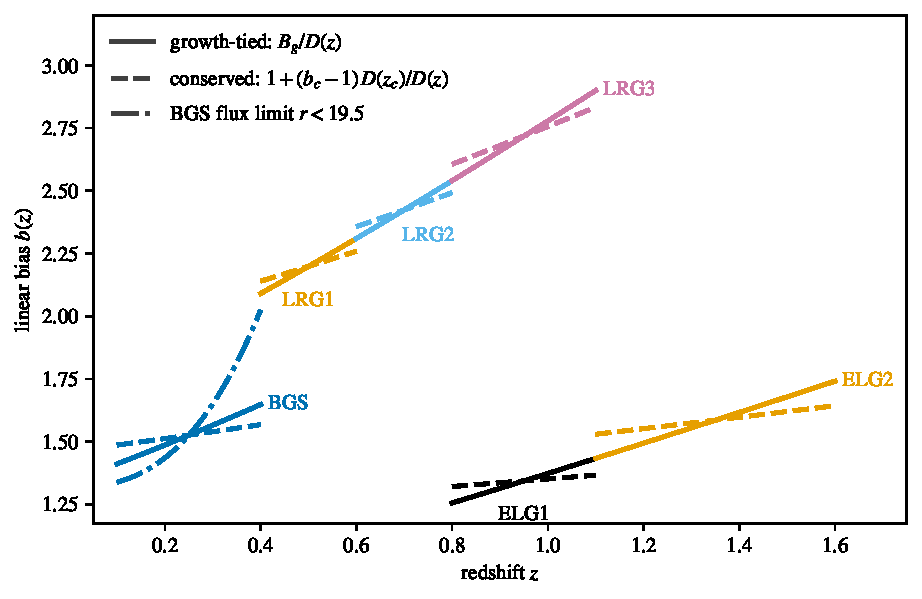
\includegraphics[width=\linewidth]{plots/theory_bz/theory_bz.pdf}
  \caption{The bias $b(z)$ of every group.  Solid: the growth-tied
    shape $B_g/D(z)$.  Dashed: a conserved population anchored at the
    group midpoint (Eq.~\eqref{eq:fry}).  Dash-dot, on BGS only: the
    $r < 19.5$ flux-limit bias, anchored at the same midpoint.}
  \label{fig:theorybz}
\end{figure}

\subsection{What breaks conservation in a selected sample}
\label{sec:selection}

\begin{itemize}
  \item \textbf{Threshold drift.}  A selection holds a roughly constant
    comoving density until the flux limit bites; beyond, it keeps only
    its brighter, more biased members.  The change is smooth, with $L$
    comparable to the group width.
  \item \textbf{Color-selection features.}  A spectral feature crossing
    a filter edge moves a color cut quickly in redshift.  The sharpest
    is the $4000$~\AA\ break, the step in an old galaxy's rest-frame
    spectrum at $4000$~\AA, which redshift slides across the filters: a
    filter edge $100$--$200$~\AA\ wide maps to
    $\Delta z = \Delta\lambda/(4000~\text{\AA}) \approx 0.03$--$0.05$.  The crossing is known; its
    amplitude in bias is unmeasured.
  \item \textbf{Mergers} turn two members into one.
  \item \textbf{Emission-line selection.}  An ELG belongs to the sample
    while its lines are strong, so membership follows the
    star-formation phase.
\end{itemize}

\subsection{What the measurements say}
\label{sec:evidence}

Each statement is tagged \emph{measured} (read from the cited source),
\emph{derived} (computed here from measured inputs) or \emph{assumed}.
Equation~\eqref{eq:fry} is from Fry~\cite{Fry1996};
Tegmark and Peebles~\cite{TegmarkPeebles1998} rederive it.

\paragraph{Massive red galaxies follow the conserved shape.}
SDSS and 2SLAQ LRGs at $0.19 < z < 0.55$, matched in color and
luminosity, show no significant evolution of the clustering amplitude
and merge at $7.5 \pm 2.3\%$ over that range, about $2.4\%$ per
Gyr~\cite{Wake2008} (measured).  The BOSS progenitors of the SDSS LRGs
merge at $2 \pm 1.5\%$ per Gyr and cluster as the continuity equation
predicts~\cite{Tojeiro2012}, and CMASS samples of fixed comoving
density at $0.43 < z < 0.7$ cluster like a conserved
population~\cite{Guo2013} (measured).  The bias of DESI-like LRGs in
photometric bins of $\Delta z \approx 0.1$ stays within $\pm 2.3\%$ of
$b = 1.5/D$ below $z = 0.83$, with the highest bin $6.4 \pm 6.4\%$
high~\cite{Zhou2021} (measured biases, residuals derived;
Figure~\ref{fig:zhou}).

\begin{figure}[htbp]
  \centering
  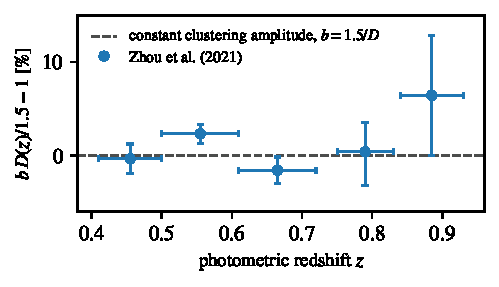
\includegraphics{plots/zhou_lrg_bias/zhou_lrg_bias.pdf}
  \caption{The measured bias of DESI-like LRGs~\cite{Zhou2021} as a
    fractional residual around $b = 1.5/D$, with $D$ at each
    photometric bin's center (flat $\Lambda$CDM, $\Omega_m = 0.3$);
    horizontal bars: the bin edges.}
  \label{fig:zhou}
\end{figure}

\paragraph{The selections drift.}
The DESI LRG cuts hold the comoving density near
$5 \times 10^{-4}\,(h/{\rm Mpc})^3$ at $0.4 < z < 0.8$ and hand over to
a fixed flux limit beyond~\cite{Zhou2023lrg} (measured).  That limit
raises the luminosity threshold by $0.27$ magnitudes per
$\Delta z = 0.1$ at $z \approx 1$; times the threshold-bias slope of
SDSS luminosity-threshold samples, $b\,(\sigma_8/0.8) = 1.06 +
0.21\,(L_{\rm th}/L_*)^{1.12}$~\cite{Zehavi2011} ($0.5$--$1.0$ in bias
per magnitude near LRG luminosities; measured), it drifts the LRG3 bias
by $6$--$11\%$ per $\Delta z = 0.1$ on top of $B/D$ (derived, from an
$r$-band relation outside its calibrated range, so only the direction
and order of magnitude hold).  BGS Bright is magnitude limited at
$r < 19.5$~\cite{Hahn2023} (measured), which drives a $10$--$25\%$ bias
drift across the group (derived; Appendix~\ref{app:bgsflux}).

\paragraph{The ELG bias shape is stable.}
Fits of the halo occupation distribution (HOD: how many sample
galaxies live in a halo of each mass) to the DESI One-Percent ELGs in
$0.8 < z < 1.1$ and
$1.1 < z < 1.6$ agree within one sigma~\cite{Rocher2023} (measured);
at these host masses the halo bias depends weakly on mass, so the
implied drift is at the percent level (derived, slope assumed).  The
[OII] doublet loses signal-to-noise in windows
$\Delta z \approx 0.001$--$0.01$ wide where it lands on sky lines,
especially at $z > 1.5$~\cite{Raichoor2023} (measured): the one
short-separation mechanism with a measured location, with an assumed
bias amplitude of $1$--$2\%$.

\paragraph{Nothing resolves bias below $\Delta z \approx 0.1$.}
The CMB-lensing tomography of the same samples~\cite{White2022,
Sailer2024, Sailer2025}, on the photometric samples of
Zhou et al.~\cite{Zhou2023tomo}, uses bins of about $0.15$ with one
free bias per bin and finds smooth models that fit.  Below
$\Delta z \approx 0.1$ this note rests on the continuity equation and
the selection arguments.

\section{The memory model}
\label{sec:memory}

\subsection{Why a second model}
\label{sec:memwhy}

Every deviation above except the sky-line windows is a monotonic drift:
the conserved-population tilt (about $1\%$ per $\Delta z = 0.05$), the
LRG3 magnitude-limit drift ($6$--$11\%$ per $\Delta z = 0.1$) and the
BGS flux-limit drift ($10$--$25\%$ across the group).  The kernel model
admits such a drift only at a price: to pass a $20\%$ drift with
$L \leq 0.1$ it takes $\sigma_g = 10$--$15\%$, which also allows about
$10\%$ scatter between neighbors that no identified mechanism
produces.  One $\sigma_g$ controls both, so the kernel cannot say
``large smooth drift, small local scatter''.  The memory model
separates the two.

\subsection{Why the kernel forgets}
\label{sec:memforget}

At $L = 0.05$, bins $0.15$ apart share $e^{-3} \approx 0.05$ of their
deviation.  With $r_k = e^{-(\bar{z}_{k+1} - \bar{z}_k)/L}$ the
correlation of neighbors $k$ and $k+1$, the best guess of the next bin
given all earlier ones is (Appendix~\ref{app:chain})
\begin{equation}
  \mathrm{E}\bigl[\delta_{k+1} \mid \delta_1, \dots, \delta_k\bigr]
  \;=\; r_k\, \delta_k :
  \label{eq:memmarkov}
\end{equation}
only the nearest neighbor matters, and the influence of any one bin
fades along the chain.

\subsection{The model, and why it remembers}
\label{sec:memmodel}

The memory model adds a tilt per group and splits the deviation into a
line and a residual,
\begin{equation}
  \delta_i \;=\; s_g\, v_i + \varepsilon_i,
  \qquad
  v_i \;=\; \bar{z}_i - \bar{z}_g,
  \label{eq:memdef}
\end{equation}
with $s_g$ a free tilt (flat prior, like $B_g$) and $\varepsilon_i$
carrying the kernel of Eq.~\eqref{eq:priorkernel}: the model of
Eqs.~\eqref{eq:summodel} and \eqref{eq:sumkernel}.  Giving the slope a
Gaussian prior of variance $\tau^2$ first (the flat prior is
$\tau \to \infty$), the deviations have covariance
\begin{equation}
  \mathrm{Cov}(\delta_i, \delta_j)
  \;=\;
  \tau^2\, v_i\, v_j
  \;+\;
  \sigma_g^2\, e^{-|\bar{z}_i - \bar{z}_j|/L} .
  \label{eq:memcov}
\end{equation}
The new term does not decay with separation.  Far beyond $L$ the
correlation coefficient tends to
\begin{equation}
  \rho_{ij}
  \;\longrightarrow\;
  \frac{\tau^2 v_i v_j}
       {\sqrt{\bigl(\tau^2 v_i^2 + \sigma_g^2\bigr)
              \bigl(\tau^2 v_j^2 + \sigma_g^2\bigr)}}
  \;\longrightarrow\; \pm 1
  \quad \text{when } \tau |v| \gg \sigma_g :
  \label{eq:memrho}
\end{equation}
the two ends of a group remember each other through the shared slope.
The best guess of the next bin becomes
\begin{equation}
  \mathrm{E}\bigl[\delta_{k+1} \mid \delta_1, \dots, \delta_k\bigr]
  \;=\;
  \hat{c} + \hat{s}_g\, v_{k+1}
  \;+\;
  r_k\,\bigl(\delta_k - \hat{c} - \hat{s}_g\, v_k\bigr),
  \label{eq:memkriging}
\end{equation}
with $(\hat{c}, \hat{s}_g)$ the level and slope of the best straight
line through all past bins, weighted by $\Cov^{-1}$: every past bin
enters through the fitted line, and only the wiggle around it stays
Markov (the universal-kriging predictor; kriging is the geostatistics
name for the best linear prediction from correlated data;
Appendix~\ref{app:memory}).
Figure~\ref{fig:theorydraws} shows the difference on the BGS bins at
$\Delta z = 0.02$: kernel draws wide enough to admit the BGS drift
zigzag and forget, while memory draws are lines with small wiggles,
among which the drift looks typical.

\begin{figure}[htbp]
  \centering
  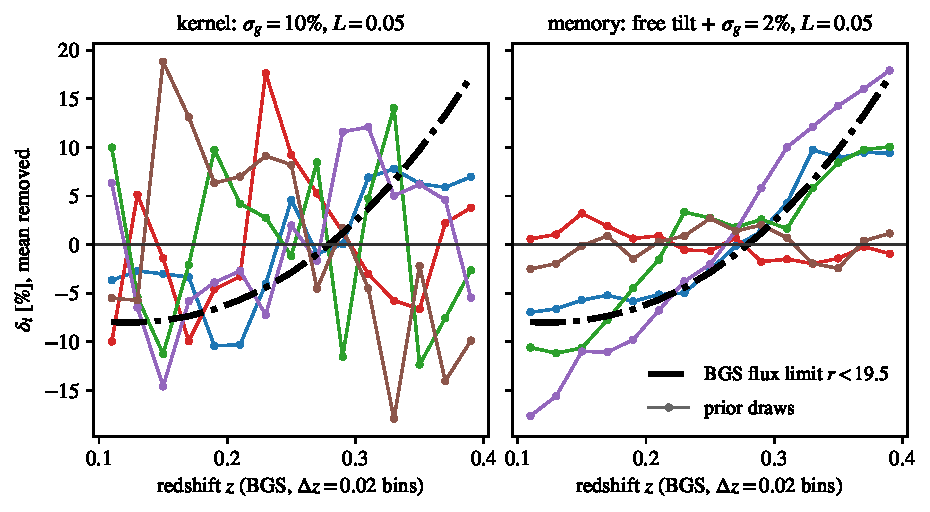
\includegraphics[width=\linewidth]{plots/theory_draws/theory_draws.pdf}
  \caption{Random prior draws of the deviations of the 15 BGS bins at
    $\Delta z = 0.02$, each draw's mean removed ($B_g$ is free).  Thick
    dash-dot: the BGS flux-limit drift.  Left: the kernel model.
    Right: the memory model, whose tilt is free in the model and drawn
    here, for display only, from a Gaussian of width $0.6$ per unit
    redshift.}
  \label{fig:theorydraws}
\end{figure}

\subsection{Why the memory model differs physically}
\label{sec:memphysics}

A selected sample changes along a group in two ways.  Coherent changes
move every bin the same way: a threshold that rises with distance, the
debiasing of a conserved population.  Local changes move bins
independently and are forgotten over a short range: the sky-line
windows and filter-edge crossings of Appendix~\ref{sec:selection}.  The
memory model gives the first kind to the tilt and the second to the
kernel.  One line suffices for the coherent kind, because the drifts
are smooth functions of $D(z)$ and the distance modulus.  The best
equal-weight line through each group's conserved deviation at the
$\Delta z = 0.05$ bin centers (derived; amplitudes $1.34$ for BGS,
$1.70$ for the LRGs and $0.84$ for the ELGs) removes deviations that
span $3$--$11\%$ and leaves $0.02$--$0.16\%$ rms, at most $0.27\%$
(ELG2).  The BGS flux-limit drift is larger and convex: it spans
$22.3\%$, and its best line leaves $2.4\%$ rms and $3.3\%$ at most
(Appendix~\ref{app:bgsflux}).  Figure~\ref{fig:theorydelta} shows both.
In the memory model $\sigma_g$ is the departure from the group's own
line, curvature plus local scatter: about $0.1\%$ for a conserved
population, $1$--$2\%$ for local selection features, $2$--$3\%$ for the
BGS curvature.

\begin{figure}[htbp]
  \centering
  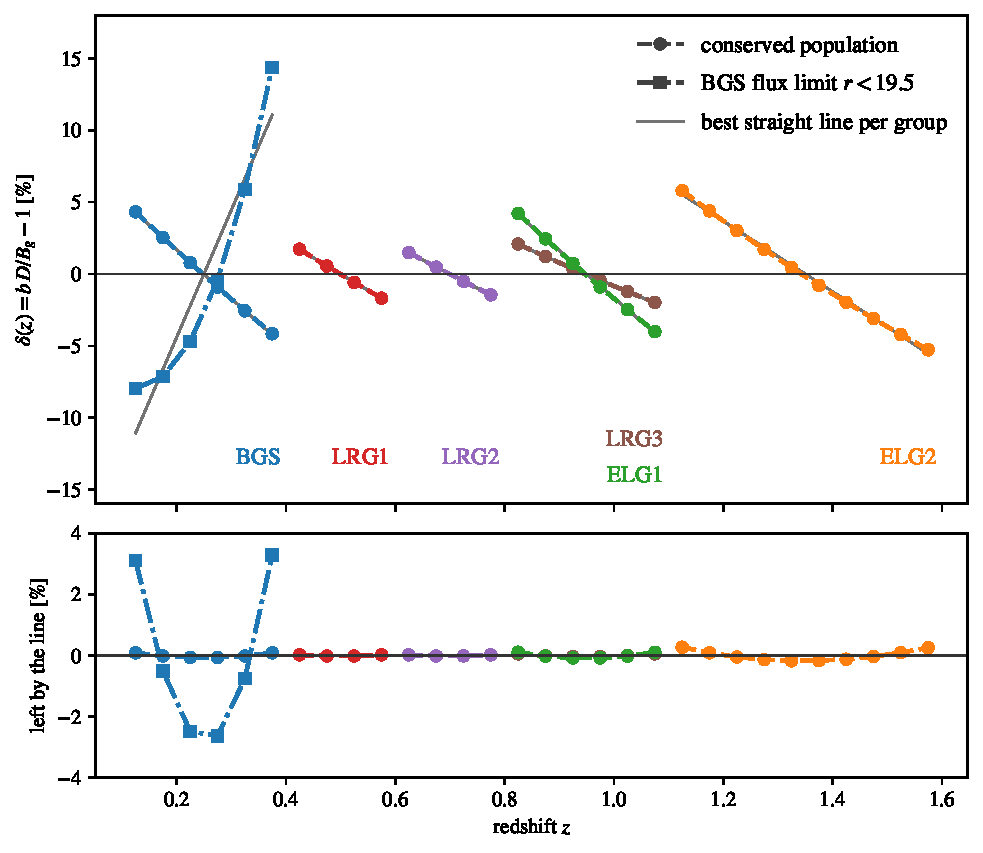
\includegraphics[width=\linewidth]{plots/theory_delta/theory_delta.pdf}
  \caption{Top: the deviation $\delta(z) = b\,D/B_g - 1$ at the
    $\Delta z = 0.05$ bin centers, with $B_g$ set so the mean deviation
    vanishes.  Dashed with circles: the conserved population, every
    group.  Dash-dot with squares: the BGS flux limit.  Thin gray: the
    best straight line per curve.  Bottom: what the line leaves.}
  \label{fig:theorydelta}
\end{figure}

\subsection{What the prior charges}
\label{sec:memcharge}

With flat priors on the line's level and slope, the prior precision of
a group's bin amplitudes is (Appendix~\ref{app:memory})
\begin{equation}
  \Prec_{\rm mem}
  \;=\;
  \mathsf{Q} - \mathsf{Q}\,\mathsf{U}
  \bigl(\mathsf{U}\T \mathsf{Q}\, \mathsf{U}\bigr)^{-1}
  \mathsf{U}\T \mathsf{Q},
  \qquad
  \mathsf{Q} = \Cov^{-1},
  \qquad
  \mathsf{U} = [\,\ones,\ v\,],
  \label{eq:memproj}
\end{equation}
the construction of Eq.~\eqref{eq:projdef} with one more column.  Its
penalty is
\begin{equation}
  \delta\T \Prec_{\rm mem}\, \delta
  \;=\;
  \min_{c,\, s_g}\;
  \bigl(\delta - c\,\ones - s_g\, v\bigr)\T
  \mathsf{Q}
  \bigl(\delta - c\,\ones - s_g\, v\bigr) :
  \label{eq:memmin}
\end{equation}
the prior subtracts the best straight line and charges only the
residual.  A monotonic drift of any size costs nothing; bumps around
the line still cost, and still forget over $L$.  $\mathsf{Q}$ is
tridiagonal (Appendix~\ref{sec:general}), while the subtracted term has
rank two and is dense, because the fitted line listens to every bin.
$\Prec_{\rm mem}\mathsf{U} = 0$, $\Prec_{\rm mem}$ is positive
semidefinite with rank $n - 2$, and a group of one or two bins has
$\Prec_{\rm mem} = 0$.

\section{The bias continuity equation, step by step}
\label{app:continuity}

The matter overdensity is $\delta_m = (\rho_m - \bar\rho_m)/\bar\rho_m$,
with $\bar\rho_m(t)$ the mean density; the galaxy-count overdensity
$\delta_{\rm gal}$ is defined the same way.  Conservation of mass and of
galaxy number gives, in comoving coordinates and to linear order (the
convective term $\mathbf{v} \cdot \nabla \delta$ is second order),
\begin{equation}
  \frac{\partial \delta_m}{\partial t}
  \;=\;
  -\,\frac{1}{a}\,\nabla \cdot \mathbf{v}_m,
  \qquad
  \frac{\partial \delta_{\rm gal}}{\partial t}
  \;=\;
  -\,\frac{1}{a}\,\nabla \cdot \mathbf{v}_{\rm gal},
  \label{eq:continuity}
\end{equation}
with $t$ cosmic time and $\mathbf{v}_m$, $\mathbf{v}_{\rm gal}$ the
peculiar velocities.  On large scales galaxies fall in the same
potential as the matter and carry no pressure of their own, so
$\mathbf{v}_{\rm gal} = \mathbf{v}_m$ (no velocity bias; galaxies as
test particles in Tegmark and Peebles~\cite{TegmarkPeebles1998}).
Subtracting the two equations and integrating from $z_c$,
\begin{equation}
  \delta_{\rm gal}(z) - \delta_m(z)
  \;=\;
  \delta_{\rm gal}(z_c) - \delta_m(z_c) :
  \label{eq:frozen}
\end{equation}
the excess clumping keeps its initial value.  With
$\delta_{\rm gal}(z_c) = b_c\,\delta_m(z_c)$ and
$\delta_m(z) = \delta_m(z_c)\, D(z)/D(z_c)$,
\begin{equation}
  \delta_{\rm gal}(z)
  \;=\;
  \delta_m(z)
  \left[\,1 + \bigl(b_c - 1\bigr)\,\frac{D(z_c)}{D(z)}\,\right],
  \label{eq:appsub}
\end{equation}
and dividing by $\delta_m(z)$ gives Eq.~\eqref{eq:fry}; dividing by the
growth-tied bias gives Eq.~\eqref{eq:tilt}.  As $D$ grows the frozen
term is divided by an ever larger number, so $b \to 1$: gravity
debiases a conserved sample.

Tegmark and Peebles also allow stochastic bias, with $b$ the ratio of
the galaxy to the matter fluctuation amplitude and $\rho_{gm}$ the
correlation coefficient of the two fields.  The same argument evolves
both: with $D$ normalized to one today and the subscript zero marking
today,
\begin{equation}
  b_0 =
  \left[(1 - D)^2 + 2 D (1 - D)\, b\, \rho_{gm}
  + D^2 b^2\right]^{1/2},
  \qquad
  \rho_{gm,0} = \frac{(1 - D) + D\, b\, \rho_{gm}}{b_0},
  \label{eq:tpevol}
\end{equation}
with $b$ and $\rho_{gm}$ the values at the epoch of growth factor $D$.
Both approach one as clustering grows, and for $\rho_{gm} = 1$
Eq.~\eqref{eq:tpevol} collapses to $b_0 - 1 = (b - 1)\,D$,
Eq.~\eqref{eq:fry} again.  For a DESI sample the assumption that
breaks is conservation (Appendix~\ref{sec:selection}); no velocity
bias and linear theory hold well on the scales kept.  The script of
Appendix~\ref{app:verify} integrates Eq.~\eqref{eq:continuity} and
recovers Eq.~\eqref{eq:fry} to $2 \times 10^{-9}$.

\section{The BGS flux-limit bias model, step by step}
\label{app:bgsflux}

This appendix derives the BGS drift of the baseline prior: a $22.3\%$
span, a convex shape, and a $2.4\%$ rms residual around the best line
(the function \texttt{bgs\_flux\_limit\_bias} of
\texttt{plots/make\_theory\_data.py}).

\subsection{The four steps}
\label{sec:bgssteps}

\paragraph{Step 1: the flux limit becomes a luminosity threshold.}
BGS Bright keeps every galaxy brighter than $r = 19.5$~\cite{Hahn2023}
($r$ the magnitude band).  The apparent magnitude $r$ and the absolute
magnitude $M$ are related by
$r = M + 25 + 5\log_{10}[d_L/(h^{-1}\,{\rm Mpc})] + K(z)$, with $d_L$
the luminosity distance and $K(z)$ the K-correction, the magnitude
correction for the part of the redshifted spectrum that falls outside
the observed band~\cite{BlantonRoweis2007}.  With $K = 0$ the faintest
absolute magnitude that passes at redshift $z$ is
\begin{equation}
  M_{\rm lim}(z) - 5\log_{10} h
  \;=\;
  19.5 - 25 - 5\log_{10} \frac{d_L(z)}{h^{-1}\,{\rm Mpc}},
  \qquad
  d_L(z) \;=\; (1+z)\,\chi(z),
  \label{eq:bgsmlim}
\end{equation}
with $\chi(z)$ the comoving distance of flat $\Lambda$CDM with
$\Omega_m = 0.3$ and $h$ the Hubble constant in units of
$100$~km/s/Mpc.

\paragraph{Steps 2 and 3: each bin is a threshold sample, and the
threshold sets the bias.}
At redshift $z$ the sample holds every galaxy with
$M < M_{\rm lim}(z)$, a threshold that brightens with distance.  The
SDSS luminosity-threshold samples at $z < 0.25$~\cite{Zehavi2011}
give
\begin{equation}
  b(>L_{\rm th})
  \;=\;
  1.06 + 0.21\,(L_{\rm th}/L_*)^{1.12},
  \qquad
  L_{\rm th}/L_* \;=\; 10^{-0.4\,(M_{\rm lim} - M_*)},
  \label{eq:bgszehavi}
\end{equation}
with $M_* - 5\log_{10} h = -20.44$ the characteristic magnitude of the
SDSS $r$-band luminosity function~\cite{Blanton2003}.  The model
applies the fit at every redshift, without evolution, and reads the
published $b\,(\sigma_8/0.8)$ as $b$.

\paragraph{Step 4: the deviation from the growth-tied shape.}
Because $B_g$ is free, only the shape of $b(z)$ matters; the amplitude
makes the mean deviation over the group's bin centers vanish:
\begin{equation}
  \delta(\bar{z}_i)
  \;=\;
  \frac{b(\bar{z}_i)\,D(\bar{z}_i)}{B} - 1,
  \qquad
  B \;=\; \frac{1}{n}\sum_{j=1}^{n} b(\bar{z}_j)\,D(\bar{z}_j).
  \label{eq:bgsdelta}
\end{equation}
At the six $\Delta z = 0.05$ bin centers of BGS, $z = 0.125$ to
$0.375$, the threshold brightens from $-18.56$ to $-21.24$, so
$L_{\rm th}/L_*$ grows from $0.18$ to $2.10$ and the bias from $1.09$
to $1.54$, while $D$ falls from $0.937$ to $0.824$.  The deviation runs
from $-8.0\%$ to $+14.4\%$, the $22.3\%$ span of
Figure~\ref{fig:theorydelta}.

\subsection{Why the drift is convex}
\label{sec:bgsconvex}

The bias rises by $41\%$ while $D$ falls by $12\%$, so the deviation
inherits the shape of the bias curve, which is flat at low redshift
and steep at high redshift: below $L_*$ the term
$0.21\,(L_{\rm th}/L_*)^{1.12}$ is small against $1.06$ ($0.03$ at the
first center), the threshold crosses $L_*$ near $z = 0.27$, and beyond
it the term rises exponentially ($0.48$ at the last center).  A
straight line through a convex curve leaves a U-shaped residual,
$(+3.1, -0.5, -2.5, -2.6, -0.8, +3.3)\%$ here.  Adding a quadratic term
cuts the residual from $2.4\%$ to $0.1\%$ rms, so the $2.4\%$ is the
curvature of the drift, the one part a free tilt cannot absorb.

\subsection{What the model leaves out}
\label{sec:bgsomissions}

None of the omissions changes the qualitative shape, a smooth,
monotonic, convex rise toward the far edge of the group.
\begin{itemize}
  \item \textbf{Evolution of the threshold-bias relation.}  The bias at
    fixed luminosity grows with redshift (Eq.~\eqref{eq:fry}), which
    steepens the drift; $M_*$ brightens by $1$--$2$ magnitudes per unit
    redshift~\cite{Blanton2003}, which flattens it, but only by
    $0.3$--$0.6$ magnitudes at the last center against the $2.68$ of
    the threshold.
  \item \textbf{No K-correction.}  A positive $K$, $0.37$ magnitudes at
    $z = 0.4$ for a spectrum flat in wavelength and more for a red
    one~\cite{BlantonRoweis2007}, makes the true threshold brighter at
    high redshift and steepens the drift.
  \item \textbf{Only $r < 19.5$.}  BGS Faint, at
    $19.5 < r < 20.175$~\cite{Hahn2023}, lowers the threshold by $0.675$
    magnitudes and flattens the drift; the fiber-magnitude cut and the
    color selection change the galaxy mix in a way
    Eq.~\eqref{eq:bgszehavi} cannot follow.
\end{itemize}
The model is an order-of-magnitude estimate, not a prediction of the
measured DESI BGS bias.  Its reliable content is the shape of the drift
and its size to a factor of order unity, which is what the baseline
prior uses: $\sigma_g = 3\%$ for BGS, from the $2$--$3\%$ curvature.
 right after \appendix.  No preamble: the
% macros \ones, \Prec, \Cov and \T come from the main file.  The labels
% are shared with the mathematics appendices (appendix_math.tex).

\section{The models}
\label{sec:models}

This appendix first builds the prior without the tilt of
Eq.~\eqref{eq:summodel}: the kernel model, in which the exponential
kernel describes the whole deviation $\delta_i$ of a bin from its
group's trend.  Appendix~\ref{sec:memory} adds the free tilt, and the
kernel then describes the residual $\varepsilon_i$ around each group's
line.  In the appendices $b_i$ is the linear bias $b_{1,i}$ of bin $i$.

\subsection{Growth-tied, free, and correlated biases}
\label{sec:defs}

The growth-tied model sets $b_i = B_g/D(\bar{z}_i)$, with one free
amplitude $B_g$ per group.  The kernel model multiplies it by a
fractional deviation $\delta_i$,
\begin{align}
  b_i &\;=\; \frac{B_g}{D(\bar{z}_i)}\,\bigl(1 + \delta_i\bigr),
  \label{eq:model}
  \\
  \bigl\langle \delta_i\,\delta_j \bigr\rangle
  &\;=\; \sigma_g^2\,
  \exp\!\left(-\,\frac{|\bar{z}_i - \bar{z}_j|}{L}\right),
  \label{eq:priorkernel}
\end{align}
with $B_g$ still free (flat prior) and the prior zero across groups.
In the Fisher matrix the convenient parameters are the per-bin
amplitudes
\begin{equation}
  \beta_i \;\equiv\; B_g\,\bigl(1 + \delta_i\bigr),
  \qquad \text{fiducial } \beta_i = B_g,
  \label{eq:beta}
\end{equation}
so that $b_i = \beta_i / D(\bar{z}_i)$.  Since
$\beta_i - B_g = B_g\,\delta_i$, the prior covariance of the $\beta_i$
within one group is
\begin{equation}
  \Cov \;=\; \sigma_\beta^2\,\mathsf{R},
  \qquad
  \sigma_\beta \;=\; \sigma_g\,B_g,
  \qquad
  \mathsf{R}_{ij} \;=\; \exp\!\left(-\,\frac{|\bar{z}_i - \bar{z}_j|}{L}\right),
  \label{eq:covdef}
\end{equation}
with $\sigma_\beta$ the spread of one amplitude, in units of a bias, and
$\mathsf{R}$ the dimensionless correlation matrix.

\subsection{What $\sigma_g$ and $L$ mean}
\label{sec:jump}

The diagonal of the kernel gives the wander of a single bin,
$\mathrm{Var}(\delta_i) = \sigma_g^2$.  The correlation coefficient of
two bins at separation $\Delta z = |\bar{z}_i - \bar{z}_j|$ is
\begin{equation}
  r \;=\;
  \frac{\langle \delta_i \delta_j \rangle}
       {\sqrt{\langle \delta_i^2 \rangle\,\langle \delta_j^2 \rangle}}
  \;=\; e^{-\Delta z / L} ,
  \label{eq:rdef}
\end{equation}
set by the separation and $L$ alone.  The jump between the two bins has
variance
\begin{equation}
  \mathrm{Var}(\delta_i - \delta_j)
  \;=\;
  2\,\sigma_g^2\left(1 - e^{-\Delta z / L}\right)
  \;\approx\;
  \frac{2\,\sigma_g^2\,\Delta z}{L}
  \quad (\Delta z \ll L).
  \label{eq:jumpvar}
\end{equation}
At small separations the jump variance grows linearly with
$\Delta z$, as for a random walk; only beyond $L$ does the finite
wander pull the deviation back.  For neighbors at $\Delta z = 0.02$
with $L = 0.05$, $r = e^{-0.4} = 0.670$ and the exact rms jump is
$0.81\,\sigma_g$; the small-separation form gives $0.89\,\sigma_g$,
because $\Delta z/L = 0.4$ is not small.

\subsection{The free group amplitude and the projection}
\label{sec:projintro}

A plain Gaussian prior with covariance $\Cov$ would charge for moving
all $\beta_i$ of a group together, but that uniform shift is the free
amplitude $B_g$.  The repair removes the uniform direction: with
$\ones$ the ones vector of the group's $n$ bins, the prior precision
of a group's amplitudes is
\begin{equation}
  \Prec \;=\; \Cov^{-1}
  \;-\;
  \frac{\Cov^{-1}\ones\,\ones\T \Cov^{-1}}{\ones\T \Cov^{-1} \ones}.
  \label{eq:projdef}
\end{equation}
$\Prec\,\ones = 0$, so a uniform shift costs nothing; a pure shape
change keeps the penalty of the plain prior; $\Prec$ is positive
semidefinite (no displacement has a negative penalty) with rank
$n - 1$; and $\Prec$ is exactly the prior
obtained by sampling $B_g$ with a flat prior and marginalizing it.
Appendices~\ref{sec:twobins}, \ref{sec:threeviews} and
\ref{sec:general} show these for two bins, by marginalization, and for
$n$ bins.  Across groups the prior is zero, so the full prior
precision is block diagonal.

\section{Which $L$ and $\sigma_g$ are physical}
\label{sec:physical}

One case of bias evolution can be solved in closed form: a population
whose members are conserved.  This appendix derives it, measures its
deviation from the growth-tied trend, lists what breaks conservation in
a selected sample, and weighs the published measurements.

\subsection{A conserved population: the bias continuity equation}
\label{sec:conserved}

Take a sample whose membership never changes, with no velocity bias,
in linear theory.  The matter overdensity $\delta_m$ and the
galaxy-count overdensity $\delta_{\rm gal}$ then obey the same
continuity equation with the same velocity field, so the excess
clumping $\delta_{\rm gal} - \delta_m$ is frozen
(Appendix~\ref{app:continuity}).  With $b_c$ the linear bias at a
reference redshift $z_c$ and $\delta_m \propto D$, the frozen
difference gives~\cite{Fry1996}
\begin{equation}
  b(z) - 1
  \;=\;
  \bigl(b_c - 1\bigr)\,\frac{D(z_c)}{D(z)} :
  \label{eq:fry}
\end{equation}
the excess set at formation stays fixed while the matter clustering
grows, so the bias decays toward one.  The growth-tied shape freezes a
different quantity: constant $b\,D$ means a galaxy clustering amplitude
$b\,\delta_m$ that does not grow, which describes a selection that
picks, at each redshift, a different and rarer set of objects.

\subsection{The deviation from the growth-tied trend}
\label{sec:tilt}

Place the reference at a group's midpoint $z_c$, with
$b_c = B/D(z_c)$.  The ratio of Eq.~\eqref{eq:fry} to the growth-tied
bias $b_c\,D(z_c)/D(z)$ gives the deviation of Eq.~\eqref{eq:model},
\begin{equation}
  \delta(z)
  \;=\;
  \frac{D(z)/D(z_c) - 1}{b_c} ,
  \label{eq:tilt}
\end{equation}
zero at the midpoint, positive at lower redshift and negative at higher
redshift, and nearly linear across a group because $D$ is smooth.  In
flat $\Lambda$CDM with $\Omega_m = 0.3$ and the project's fiducial
amplitudes it is $+5.3\%$ and $-4.9\%$ at the ends of BGS ($B = 1.34$,
$0.1 < z < 0.4$, $b_c = 1.5$), $+2.4\%$ and $-2.2\%$ at the ends of LRG1
($B = 1.70$, $0.4 < z < 0.6$, $b_c = 2.2$), and $+2.6\%$ and $-2.3\%$ at
the ends of LRG3 ($B = 1.70$, $0.8 < z < 1.1$, $b_c = 2.7$).  Between
neighbors it changes by $0.3$--$0.7\%$ at $\Delta z = 0.02$ and
$0.8$--$1.7\%$ at $\Delta z = 0.05$: a smooth tilt, coherent over the
whole group.  For comparison, the neighbor rms of
Eq.~\eqref{eq:jumpvar} at $\Delta z = 0.02$ (and $0.05$) is $2.4\%$
($3.4\%$) for $\sigma_g = 3\%$ and $L = 0.05$, and $0.44\%$ ($0.67\%$)
for $\sigma_g = 1\%$ and $L = 0.2$.  Figure~\ref{fig:theorybz} draws
these shapes: the conserved curve is flatter than $B_g/D$ in every
group, while the BGS flux-limit curve is much steeper, and convex.

\begin{figure}[htbp]
  \centering
  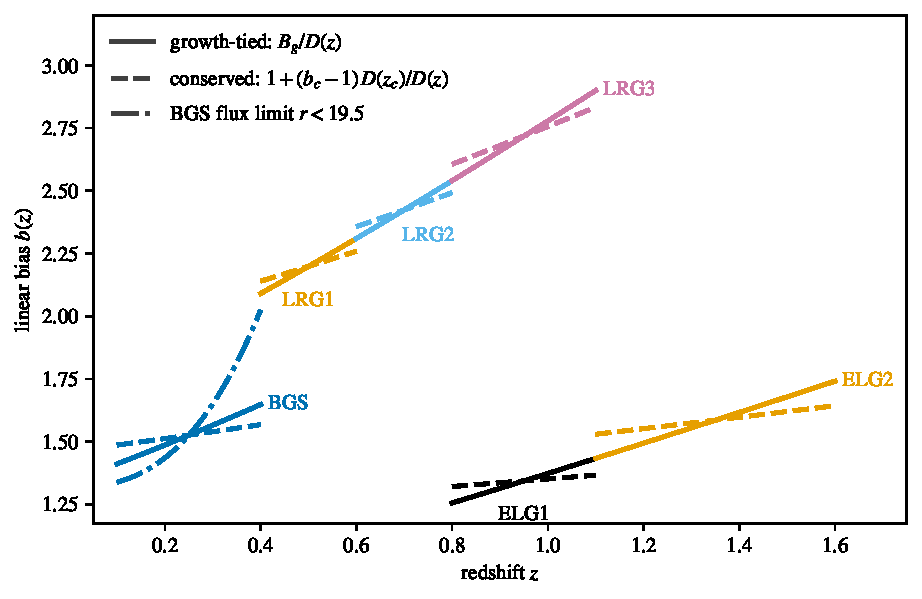
\includegraphics[width=\linewidth]{plots/theory_bz/theory_bz.pdf}
  \caption{The bias $b(z)$ of every group.  Solid: the growth-tied
    shape $B_g/D(z)$.  Dashed: a conserved population anchored at the
    group midpoint (Eq.~\eqref{eq:fry}).  Dash-dot, on BGS only: the
    $r < 19.5$ flux-limit bias, anchored at the same midpoint.}
  \label{fig:theorybz}
\end{figure}

\subsection{What breaks conservation in a selected sample}
\label{sec:selection}

\begin{itemize}
  \item \textbf{Threshold drift.}  A selection holds a roughly constant
    comoving density until the flux limit bites; beyond, it keeps only
    its brighter, more biased members.  The change is smooth, with $L$
    comparable to the group width.
  \item \textbf{Color-selection features.}  A spectral feature crossing
    a filter edge moves a color cut quickly in redshift.  The sharpest
    is the $4000$~\AA\ break, the step in an old galaxy's rest-frame
    spectrum at $4000$~\AA, which redshift slides across the filters: a
    filter edge $100$--$200$~\AA\ wide maps to
    $\Delta z = \Delta\lambda/(4000~\text{\AA}) \approx 0.03$--$0.05$.  The crossing is known; its
    amplitude in bias is unmeasured.
  \item \textbf{Mergers} turn two members into one.
  \item \textbf{Emission-line selection.}  An ELG belongs to the sample
    while its lines are strong, so membership follows the
    star-formation phase.
\end{itemize}

\subsection{What the measurements say}
\label{sec:evidence}

Each statement is tagged \emph{measured} (read from the cited source),
\emph{derived} (computed here from measured inputs) or \emph{assumed}.
Equation~\eqref{eq:fry} is from Fry~\cite{Fry1996};
Tegmark and Peebles~\cite{TegmarkPeebles1998} rederive it.

\paragraph{Massive red galaxies follow the conserved shape.}
SDSS and 2SLAQ LRGs at $0.19 < z < 0.55$, matched in color and
luminosity, show no significant evolution of the clustering amplitude
and merge at $7.5 \pm 2.3\%$ over that range, about $2.4\%$ per
Gyr~\cite{Wake2008} (measured).  The BOSS progenitors of the SDSS LRGs
merge at $2 \pm 1.5\%$ per Gyr and cluster as the continuity equation
predicts~\cite{Tojeiro2012}, and CMASS samples of fixed comoving
density at $0.43 < z < 0.7$ cluster like a conserved
population~\cite{Guo2013} (measured).  The bias of DESI-like LRGs in
photometric bins of $\Delta z \approx 0.1$ stays within $\pm 2.3\%$ of
$b = 1.5/D$ below $z = 0.83$, with the highest bin $6.4 \pm 6.4\%$
high~\cite{Zhou2021} (measured biases, residuals derived;
Figure~\ref{fig:zhou}).

\begin{figure}[htbp]
  \centering
  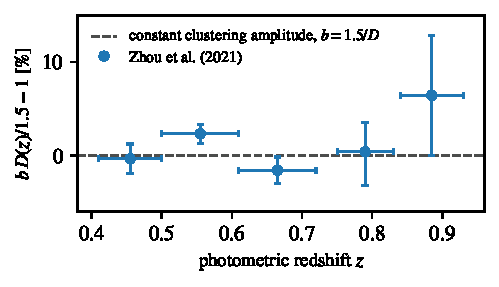
\includegraphics{plots/zhou_lrg_bias/zhou_lrg_bias.pdf}
  \caption{The measured bias of DESI-like LRGs~\cite{Zhou2021} as a
    fractional residual around $b = 1.5/D$, with $D$ at each
    photometric bin's center (flat $\Lambda$CDM, $\Omega_m = 0.3$);
    horizontal bars: the bin edges.}
  \label{fig:zhou}
\end{figure}

\paragraph{The selections drift.}
The DESI LRG cuts hold the comoving density near
$5 \times 10^{-4}\,(h/{\rm Mpc})^3$ at $0.4 < z < 0.8$ and hand over to
a fixed flux limit beyond~\cite{Zhou2023lrg} (measured).  That limit
raises the luminosity threshold by $0.27$ magnitudes per
$\Delta z = 0.1$ at $z \approx 1$; times the threshold-bias slope of
SDSS luminosity-threshold samples, $b\,(\sigma_8/0.8) = 1.06 +
0.21\,(L_{\rm th}/L_*)^{1.12}$~\cite{Zehavi2011} ($0.5$--$1.0$ in bias
per magnitude near LRG luminosities; measured), it drifts the LRG3 bias
by $6$--$11\%$ per $\Delta z = 0.1$ on top of $B/D$ (derived, from an
$r$-band relation outside its calibrated range, so only the direction
and order of magnitude hold).  BGS Bright is magnitude limited at
$r < 19.5$~\cite{Hahn2023} (measured), which drives a $10$--$25\%$ bias
drift across the group (derived; Appendix~\ref{app:bgsflux}).

\paragraph{The ELG bias shape is stable.}
Fits of the halo occupation distribution (HOD: how many sample
galaxies live in a halo of each mass) to the DESI One-Percent ELGs in
$0.8 < z < 1.1$ and
$1.1 < z < 1.6$ agree within one sigma~\cite{Rocher2023} (measured);
at these host masses the halo bias depends weakly on mass, so the
implied drift is at the percent level (derived, slope assumed).  The
[OII] doublet loses signal-to-noise in windows
$\Delta z \approx 0.001$--$0.01$ wide where it lands on sky lines,
especially at $z > 1.5$~\cite{Raichoor2023} (measured): the one
short-separation mechanism with a measured location, with an assumed
bias amplitude of $1$--$2\%$.

\paragraph{Nothing resolves bias below $\Delta z \approx 0.1$.}
The CMB-lensing tomography of the same samples~\cite{White2022,
Sailer2024, Sailer2025}, on the photometric samples of
Zhou et al.~\cite{Zhou2023tomo}, uses bins of about $0.15$ with one
free bias per bin and finds smooth models that fit.  Below
$\Delta z \approx 0.1$ this note rests on the continuity equation and
the selection arguments.

\section{The memory model}
\label{sec:memory}

\subsection{Why a second model}
\label{sec:memwhy}

Every deviation above except the sky-line windows is a monotonic drift:
the conserved-population tilt (about $1\%$ per $\Delta z = 0.05$), the
LRG3 magnitude-limit drift ($6$--$11\%$ per $\Delta z = 0.1$) and the
BGS flux-limit drift ($10$--$25\%$ across the group).  The kernel model
admits such a drift only at a price: to pass a $20\%$ drift with
$L \leq 0.1$ it takes $\sigma_g = 10$--$15\%$, which also allows about
$10\%$ scatter between neighbors that no identified mechanism
produces.  One $\sigma_g$ controls both, so the kernel cannot say
``large smooth drift, small local scatter''.  The memory model
separates the two.

\subsection{Why the kernel forgets}
\label{sec:memforget}

At $L = 0.05$, bins $0.15$ apart share $e^{-3} \approx 0.05$ of their
deviation.  With $r_k = e^{-(\bar{z}_{k+1} - \bar{z}_k)/L}$ the
correlation of neighbors $k$ and $k+1$, the best guess of the next bin
given all earlier ones is (Appendix~\ref{app:chain})
\begin{equation}
  \mathrm{E}\bigl[\delta_{k+1} \mid \delta_1, \dots, \delta_k\bigr]
  \;=\; r_k\, \delta_k :
  \label{eq:memmarkov}
\end{equation}
only the nearest neighbor matters, and the influence of any one bin
fades along the chain.

\subsection{The model, and why it remembers}
\label{sec:memmodel}

The memory model adds a tilt per group and splits the deviation into a
line and a residual,
\begin{equation}
  \delta_i \;=\; s_g\, v_i + \varepsilon_i,
  \qquad
  v_i \;=\; \bar{z}_i - \bar{z}_g,
  \label{eq:memdef}
\end{equation}
with $s_g$ a free tilt (flat prior, like $B_g$) and $\varepsilon_i$
carrying the kernel of Eq.~\eqref{eq:priorkernel}: the model of
Eqs.~\eqref{eq:summodel} and \eqref{eq:sumkernel}.  Giving the slope a
Gaussian prior of variance $\tau^2$ first (the flat prior is
$\tau \to \infty$), the deviations have covariance
\begin{equation}
  \mathrm{Cov}(\delta_i, \delta_j)
  \;=\;
  \tau^2\, v_i\, v_j
  \;+\;
  \sigma_g^2\, e^{-|\bar{z}_i - \bar{z}_j|/L} .
  \label{eq:memcov}
\end{equation}
The new term does not decay with separation.  Far beyond $L$ the
correlation coefficient tends to
\begin{equation}
  \rho_{ij}
  \;\longrightarrow\;
  \frac{\tau^2 v_i v_j}
       {\sqrt{\bigl(\tau^2 v_i^2 + \sigma_g^2\bigr)
              \bigl(\tau^2 v_j^2 + \sigma_g^2\bigr)}}
  \;\longrightarrow\; \pm 1
  \quad \text{when } \tau |v| \gg \sigma_g :
  \label{eq:memrho}
\end{equation}
the two ends of a group remember each other through the shared slope.
The best guess of the next bin becomes
\begin{equation}
  \mathrm{E}\bigl[\delta_{k+1} \mid \delta_1, \dots, \delta_k\bigr]
  \;=\;
  \hat{c} + \hat{s}_g\, v_{k+1}
  \;+\;
  r_k\,\bigl(\delta_k - \hat{c} - \hat{s}_g\, v_k\bigr),
  \label{eq:memkriging}
\end{equation}
with $(\hat{c}, \hat{s}_g)$ the level and slope of the best straight
line through all past bins, weighted by $\Cov^{-1}$: every past bin
enters through the fitted line, and only the wiggle around it stays
Markov (the universal-kriging predictor; kriging is the geostatistics
name for the best linear prediction from correlated data;
Appendix~\ref{app:memory}).
Figure~\ref{fig:theorydraws} shows the difference on the BGS bins at
$\Delta z = 0.02$: kernel draws wide enough to admit the BGS drift
zigzag and forget, while memory draws are lines with small wiggles,
among which the drift looks typical.

\begin{figure}[htbp]
  \centering
  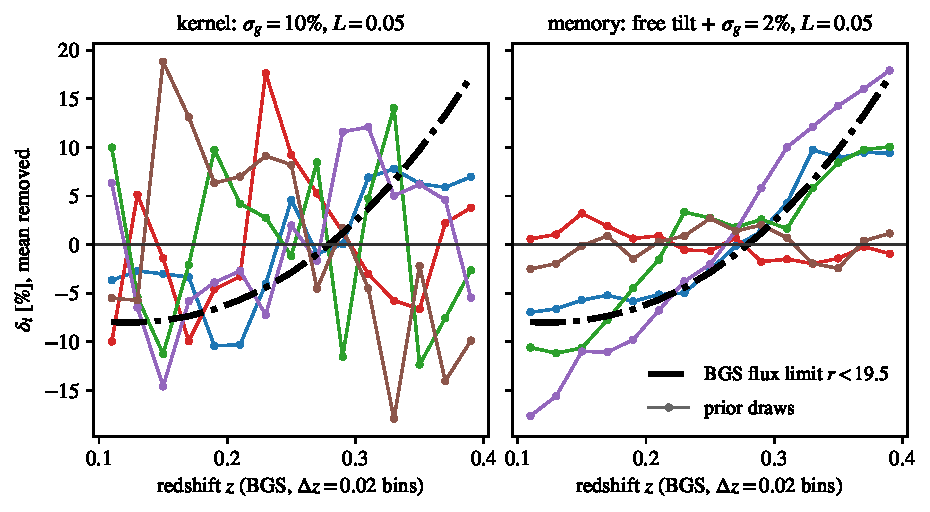
\includegraphics[width=\linewidth]{plots/theory_draws/theory_draws.pdf}
  \caption{Random prior draws of the deviations of the 15 BGS bins at
    $\Delta z = 0.02$, each draw's mean removed ($B_g$ is free).  Thick
    dash-dot: the BGS flux-limit drift.  Left: the kernel model.
    Right: the memory model, whose tilt is free in the model and drawn
    here, for display only, from a Gaussian of width $0.6$ per unit
    redshift.}
  \label{fig:theorydraws}
\end{figure}

\subsection{Why the memory model differs physically}
\label{sec:memphysics}

A selected sample changes along a group in two ways.  Coherent changes
move every bin the same way: a threshold that rises with distance, the
debiasing of a conserved population.  Local changes move bins
independently and are forgotten over a short range: the sky-line
windows and filter-edge crossings of Appendix~\ref{sec:selection}.  The
memory model gives the first kind to the tilt and the second to the
kernel.  One line suffices for the coherent kind, because the drifts
are smooth functions of $D(z)$ and the distance modulus.  The best
equal-weight line through each group's conserved deviation at the
$\Delta z = 0.05$ bin centers (derived; amplitudes $1.34$ for BGS,
$1.70$ for the LRGs and $0.84$ for the ELGs) removes deviations that
span $3$--$11\%$ and leaves $0.02$--$0.16\%$ rms, at most $0.27\%$
(ELG2).  The BGS flux-limit drift is larger and convex: it spans
$22.3\%$, and its best line leaves $2.4\%$ rms and $3.3\%$ at most
(Appendix~\ref{app:bgsflux}).  Figure~\ref{fig:theorydelta} shows both.
In the memory model $\sigma_g$ is the departure from the group's own
line, curvature plus local scatter: about $0.1\%$ for a conserved
population, $1$--$2\%$ for local selection features, $2$--$3\%$ for the
BGS curvature.

\begin{figure}[htbp]
  \centering
  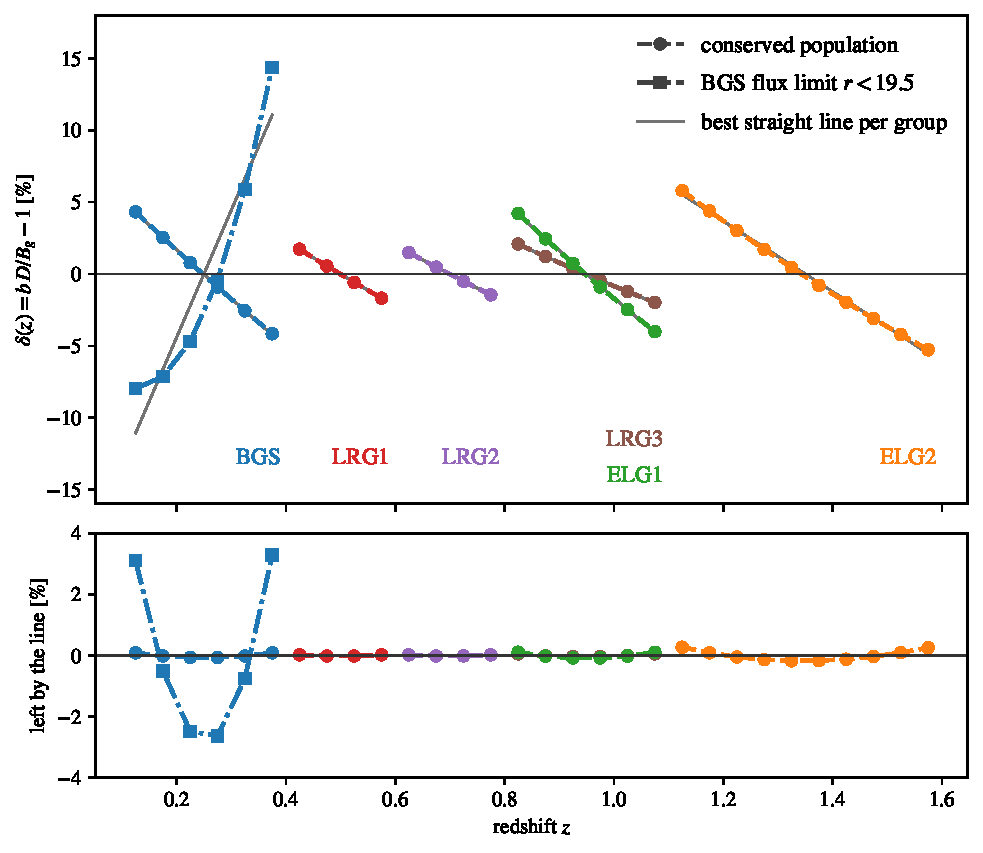
\includegraphics[width=\linewidth]{plots/theory_delta/theory_delta.pdf}
  \caption{Top: the deviation $\delta(z) = b\,D/B_g - 1$ at the
    $\Delta z = 0.05$ bin centers, with $B_g$ set so the mean deviation
    vanishes.  Dashed with circles: the conserved population, every
    group.  Dash-dot with squares: the BGS flux limit.  Thin gray: the
    best straight line per curve.  Bottom: what the line leaves.}
  \label{fig:theorydelta}
\end{figure}

\subsection{What the prior charges}
\label{sec:memcharge}

With flat priors on the line's level and slope, the prior precision of
a group's bin amplitudes is (Appendix~\ref{app:memory})
\begin{equation}
  \Prec_{\rm mem}
  \;=\;
  \mathsf{Q} - \mathsf{Q}\,\mathsf{U}
  \bigl(\mathsf{U}\T \mathsf{Q}\, \mathsf{U}\bigr)^{-1}
  \mathsf{U}\T \mathsf{Q},
  \qquad
  \mathsf{Q} = \Cov^{-1},
  \qquad
  \mathsf{U} = [\,\ones,\ v\,],
  \label{eq:memproj}
\end{equation}
the construction of Eq.~\eqref{eq:projdef} with one more column.  Its
penalty is
\begin{equation}
  \delta\T \Prec_{\rm mem}\, \delta
  \;=\;
  \min_{c,\, s_g}\;
  \bigl(\delta - c\,\ones - s_g\, v\bigr)\T
  \mathsf{Q}
  \bigl(\delta - c\,\ones - s_g\, v\bigr) :
  \label{eq:memmin}
\end{equation}
the prior subtracts the best straight line and charges only the
residual.  A monotonic drift of any size costs nothing; bumps around
the line still cost, and still forget over $L$.  $\mathsf{Q}$ is
tridiagonal (Appendix~\ref{sec:general}), while the subtracted term has
rank two and is dense, because the fitted line listens to every bin.
$\Prec_{\rm mem}\mathsf{U} = 0$, $\Prec_{\rm mem}$ is positive
semidefinite with rank $n - 2$, and a group of one or two bins has
$\Prec_{\rm mem} = 0$.

\section{The bias continuity equation, step by step}
\label{app:continuity}

The matter overdensity is $\delta_m = (\rho_m - \bar\rho_m)/\bar\rho_m$,
with $\bar\rho_m(t)$ the mean density; the galaxy-count overdensity
$\delta_{\rm gal}$ is defined the same way.  Conservation of mass and of
galaxy number gives, in comoving coordinates and to linear order (the
convective term $\mathbf{v} \cdot \nabla \delta$ is second order),
\begin{equation}
  \frac{\partial \delta_m}{\partial t}
  \;=\;
  -\,\frac{1}{a}\,\nabla \cdot \mathbf{v}_m,
  \qquad
  \frac{\partial \delta_{\rm gal}}{\partial t}
  \;=\;
  -\,\frac{1}{a}\,\nabla \cdot \mathbf{v}_{\rm gal},
  \label{eq:continuity}
\end{equation}
with $t$ cosmic time and $\mathbf{v}_m$, $\mathbf{v}_{\rm gal}$ the
peculiar velocities.  On large scales galaxies fall in the same
potential as the matter and carry no pressure of their own, so
$\mathbf{v}_{\rm gal} = \mathbf{v}_m$ (no velocity bias; galaxies as
test particles in Tegmark and Peebles~\cite{TegmarkPeebles1998}).
Subtracting the two equations and integrating from $z_c$,
\begin{equation}
  \delta_{\rm gal}(z) - \delta_m(z)
  \;=\;
  \delta_{\rm gal}(z_c) - \delta_m(z_c) :
  \label{eq:frozen}
\end{equation}
the excess clumping keeps its initial value.  With
$\delta_{\rm gal}(z_c) = b_c\,\delta_m(z_c)$ and
$\delta_m(z) = \delta_m(z_c)\, D(z)/D(z_c)$,
\begin{equation}
  \delta_{\rm gal}(z)
  \;=\;
  \delta_m(z)
  \left[\,1 + \bigl(b_c - 1\bigr)\,\frac{D(z_c)}{D(z)}\,\right],
  \label{eq:appsub}
\end{equation}
and dividing by $\delta_m(z)$ gives Eq.~\eqref{eq:fry}; dividing by the
growth-tied bias gives Eq.~\eqref{eq:tilt}.  As $D$ grows the frozen
term is divided by an ever larger number, so $b \to 1$: gravity
debiases a conserved sample.

Tegmark and Peebles also allow stochastic bias, with $b$ the ratio of
the galaxy to the matter fluctuation amplitude and $\rho_{gm}$ the
correlation coefficient of the two fields.  The same argument evolves
both: with $D$ normalized to one today and the subscript zero marking
today,
\begin{equation}
  b_0 =
  \left[(1 - D)^2 + 2 D (1 - D)\, b\, \rho_{gm}
  + D^2 b^2\right]^{1/2},
  \qquad
  \rho_{gm,0} = \frac{(1 - D) + D\, b\, \rho_{gm}}{b_0},
  \label{eq:tpevol}
\end{equation}
with $b$ and $\rho_{gm}$ the values at the epoch of growth factor $D$.
Both approach one as clustering grows, and for $\rho_{gm} = 1$
Eq.~\eqref{eq:tpevol} collapses to $b_0 - 1 = (b - 1)\,D$,
Eq.~\eqref{eq:fry} again.  For a DESI sample the assumption that
breaks is conservation (Appendix~\ref{sec:selection}); no velocity
bias and linear theory hold well on the scales kept.  The script of
Appendix~\ref{app:verify} integrates Eq.~\eqref{eq:continuity} and
recovers Eq.~\eqref{eq:fry} to $2 \times 10^{-9}$.

\section{The BGS flux-limit bias model, step by step}
\label{app:bgsflux}

This appendix derives the BGS drift of the baseline prior: a $22.3\%$
span, a convex shape, and a $2.4\%$ rms residual around the best line
(the function \texttt{bgs\_flux\_limit\_bias} of
\texttt{plots/make\_theory\_data.py}).

\subsection{The four steps}
\label{sec:bgssteps}

\paragraph{Step 1: the flux limit becomes a luminosity threshold.}
BGS Bright keeps every galaxy brighter than $r = 19.5$~\cite{Hahn2023}
($r$ the magnitude band).  The apparent magnitude $r$ and the absolute
magnitude $M$ are related by
$r = M + 25 + 5\log_{10}[d_L/(h^{-1}\,{\rm Mpc})] + K(z)$, with $d_L$
the luminosity distance and $K(z)$ the K-correction, the magnitude
correction for the part of the redshifted spectrum that falls outside
the observed band~\cite{BlantonRoweis2007}.  With $K = 0$ the faintest
absolute magnitude that passes at redshift $z$ is
\begin{equation}
  M_{\rm lim}(z) - 5\log_{10} h
  \;=\;
  19.5 - 25 - 5\log_{10} \frac{d_L(z)}{h^{-1}\,{\rm Mpc}},
  \qquad
  d_L(z) \;=\; (1+z)\,\chi(z),
  \label{eq:bgsmlim}
\end{equation}
with $\chi(z)$ the comoving distance of flat $\Lambda$CDM with
$\Omega_m = 0.3$ and $h$ the Hubble constant in units of
$100$~km/s/Mpc.

\paragraph{Steps 2 and 3: each bin is a threshold sample, and the
threshold sets the bias.}
At redshift $z$ the sample holds every galaxy with
$M < M_{\rm lim}(z)$, a threshold that brightens with distance.  The
SDSS luminosity-threshold samples at $z < 0.25$~\cite{Zehavi2011}
give
\begin{equation}
  b(>L_{\rm th})
  \;=\;
  1.06 + 0.21\,(L_{\rm th}/L_*)^{1.12},
  \qquad
  L_{\rm th}/L_* \;=\; 10^{-0.4\,(M_{\rm lim} - M_*)},
  \label{eq:bgszehavi}
\end{equation}
with $M_* - 5\log_{10} h = -20.44$ the characteristic magnitude of the
SDSS $r$-band luminosity function~\cite{Blanton2003}.  The model
applies the fit at every redshift, without evolution, and reads the
published $b\,(\sigma_8/0.8)$ as $b$.

\paragraph{Step 4: the deviation from the growth-tied shape.}
Because $B_g$ is free, only the shape of $b(z)$ matters; the amplitude
makes the mean deviation over the group's bin centers vanish:
\begin{equation}
  \delta(\bar{z}_i)
  \;=\;
  \frac{b(\bar{z}_i)\,D(\bar{z}_i)}{B} - 1,
  \qquad
  B \;=\; \frac{1}{n}\sum_{j=1}^{n} b(\bar{z}_j)\,D(\bar{z}_j).
  \label{eq:bgsdelta}
\end{equation}
At the six $\Delta z = 0.05$ bin centers of BGS, $z = 0.125$ to
$0.375$, the threshold brightens from $-18.56$ to $-21.24$, so
$L_{\rm th}/L_*$ grows from $0.18$ to $2.10$ and the bias from $1.09$
to $1.54$, while $D$ falls from $0.937$ to $0.824$.  The deviation runs
from $-8.0\%$ to $+14.4\%$, the $22.3\%$ span of
Figure~\ref{fig:theorydelta}.

\subsection{Why the drift is convex}
\label{sec:bgsconvex}

The bias rises by $41\%$ while $D$ falls by $12\%$, so the deviation
inherits the shape of the bias curve, which is flat at low redshift
and steep at high redshift: below $L_*$ the term
$0.21\,(L_{\rm th}/L_*)^{1.12}$ is small against $1.06$ ($0.03$ at the
first center), the threshold crosses $L_*$ near $z = 0.27$, and beyond
it the term rises exponentially ($0.48$ at the last center).  A
straight line through a convex curve leaves a U-shaped residual,
$(+3.1, -0.5, -2.5, -2.6, -0.8, +3.3)\%$ here.  Adding a quadratic term
cuts the residual from $2.4\%$ to $0.1\%$ rms, so the $2.4\%$ is the
curvature of the drift, the one part a free tilt cannot absorb.

\subsection{What the model leaves out}
\label{sec:bgsomissions}

None of the omissions changes the qualitative shape, a smooth,
monotonic, convex rise toward the far edge of the group.
\begin{itemize}
  \item \textbf{Evolution of the threshold-bias relation.}  The bias at
    fixed luminosity grows with redshift (Eq.~\eqref{eq:fry}), which
    steepens the drift; $M_*$ brightens by $1$--$2$ magnitudes per unit
    redshift~\cite{Blanton2003}, which flattens it, but only by
    $0.3$--$0.6$ magnitudes at the last center against the $2.68$ of
    the threshold.
  \item \textbf{No K-correction.}  A positive $K$, $0.37$ magnitudes at
    $z = 0.4$ for a spectrum flat in wavelength and more for a red
    one~\cite{BlantonRoweis2007}, makes the true threshold brighter at
    high redshift and steepens the drift.
  \item \textbf{Only $r < 19.5$.}  BGS Faint, at
    $19.5 < r < 20.175$~\cite{Hahn2023}, lowers the threshold by $0.675$
    magnitudes and flattens the drift; the fiber-magnitude cut and the
    color selection change the galaxy mix in a way
    Eq.~\eqref{eq:bgszehavi} cannot follow.
\end{itemize}
The model is an order-of-magnitude estimate, not a prediction of the
measured DESI BGS bias.  Its reliable content is the shape of the drift
and its size to a factor of order unity, which is what the baseline
prior uses: $\sigma_g = 3\%$ for BGS, from the $2$--$3\%$ curvature.

\IfFileExists{appendix_math.tex}{% appendix_math.tex: the mathematics and method appendices of
% correlated_bias_prior_v2.tex.  The parent note inputs this file after
% \appendix, so it has no preamble and its \section commands are
% appendix sections.  The memory model itself (sec:memory and its
% subsections) lives in appendix_physics.tex, next to the theory
% figures; the references to it below resolve through that file.
%
% The macros are defined here only when the parent has not defined
% them already.
\providecommand{\ones}{\mathbf{1}}  % the vector of ones, (1, ..., 1)^T
\providecommand{\Prec}{\mathsf{P}}  % a projected prior precision
\providecommand{\Cov}{\mathsf{C}}   % the prior covariance of the bin biases
\providecommand{\T}{^{\mathsf{T}}}
\providecommand{\bstwo}{b_{s^2}}

\section{The accuracy test}
\label{app:bias}

This appendix gives the method of Section~\ref{sec:accuracy}: the shift
of a fit under a known drift, the two drift laws, the random truths
built on them, and the statistic $\chidof$ of Eq.~\eqref{eq:gof}, whose
value is written $\eta$.

\subsection{The shift formula}
\label{sec:biasformula}

Let $m$ be the expected data vector (the band powers), $\mathsf{C}_d$
its covariance, $\mathsf{D}$ the matrix of derivatives of $m$ with
respect to the parameters (sans-serif, not the growth factor $D$), and
$F = \mathsf{D}\T \mathsf{C}_d^{-1} \mathsf{D} + F_{\rm priors}$ the
Fisher matrix of one fit, its priors included (Appendix~\ref{sec:fisher});
under model A the parameters include the variant's higher-order
parameters, marginalized like the cosmology.  If the true biases carry
a drift the fit may not express, the data vector moves by $\delta m$,
and to first order the maximum of the posterior moves by
\begin{equation}
  \delta p \;=\; F^{-1} \mathsf{D}\T \mathsf{C}_d^{-1}\, \delta m .
  \label{eq:fisherbias}
\end{equation}
The derivation is one line: the score (the gradient of the log
posterior) at the old maximum becomes
$\mathsf{D}\T \mathsf{C}_d^{-1} \delta m$ instead of zero, and the
curvature that converts a score into a displacement is $F$.  With
$\mathsf{C}_w$ the fit's marginalized $2 \times 2$ covariance of
$(w_0, w_a)$ and $\delta w$ the $(w_0, w_a)$ entries of $\delta p$, the
shift is
\begin{equation}
  \Delta_w \;=\; \sqrt{\delta w\T\, \mathsf{C}_w^{-1}\, \delta w} ,
  \label{eq:shiftw}
\end{equation}
the displacement of the dark-energy ellipse in units of its own size;
$\Omega_m$ and $A_s$ shifts are $|\delta p|/\sigma_p$.  The threshold
drawn in the figures is $1/3$, a shift that widens the effective error
by a few percent.  Both the ellipse and the response use the same fit's
$F$, so a rigid model is punished twice: it absorbs little of the drift,
and its ellipse is small.

The drift enters through the bin biases: with $\beta_i$ the amplitudes
of Eq.~\eqref{eq:beta} and $\delta_i$ the drift's fractional deviations,
$\delta m = \sum_i (\partial m / \partial \beta_i)\, B_g\, \delta_i$.
Under model A the column $\partial m/\partial \beta_i$ is the chain-rule
column of Eq.~\eqref{eq:chain} divided by $D(\bar{z}_i)$, so a drift of
$b_1$ drags $b_2$ and $\bstwo$ along through their calibrations.  For
the growth-tied prior the response is evaluated in its own parameter
basis; for the free prior the bias derivatives span the drift exactly,
so the cosmology shift vanishes, and the accuracy of that prior is
bought entirely with the information it gives up.

\subsection{The drift laws}
\label{sec:driftlaws}

Two known drifts are injected.  The conserved-population drift applies
to every group: the deviation of Eq.~\eqref{eq:tilt}, anchored at the
group's mean redshift, nearly a straight line of a few percent across
each group.  The BGS flux-limit drift applies to BGS alone: the convex
deviation of Appendix~\ref{app:bgsflux}, a $22\%$ span whose best line
leaves a $2.4\%$ rms curvature.  Both come from
\texttt{plots/make\_theory\_data.py}; only their shapes matter, because
the free amplitudes remove the level.

\subsection{Random truths}
\label{sec:randomtruths}

A random truth sets the bias of bin $i$ in group $g$ to
\begin{equation}
  b_i \;=\; \frac{B_g}{D(\bar{z}_i)}\,
  \bigl(1 + \delta_i^{\rm drift} + \varepsilon_i\bigr)
  \label{eq:randomtruth}
\end{equation}
at the fiducial cosmology.  The drift $\delta_i^{\rm drift}$ is the
known part: the flux limit in BGS and the conserved population in the
other five groups.  The residual $\varepsilon_i$ is one draw from the
Gaussian $\mathcal{N}(0, \Sigma)$ whose covariance is the kernel of one
of the two stated priors, $\Sigma_{ij} = \sigma_g^2\,
e^{-|\bar{z}_i - \bar{z}_j|/L}$ inside a group and zero across groups.
Two families of $2000$ truths are drawn, baseline and pessimistic
scatter, and every truth is fitted under every prior, each centered on
the growth-tied shape $\delta = 0$.  No fit is told which truth it
faces: the baseline prior meets truths drawn from its own prior and
truths drawn from the pessimistic prior, and is judged on both.

Because Eq.~\eqref{eq:fisherbias} is linear in $\delta m$, and
$\delta m$ is linear in the bias deviations, the $(w_0, w_a)$ rows of
the response collapse into one $2 \times n_{\rm bins}$ matrix
$\mathsf{A}$ per prior, layout and variant, with $n_{\rm bins}$ the
number of bins of the layout:
\begin{equation}
  \delta w \;=\; \mathsf{A}\,\delta,
  \qquad
  \delta_i \;=\; \delta_i^{\rm drift} + \varepsilon_i ,
  \label{eq:linearmap}
\end{equation}
so the $2000$ truths cost one matrix product.  The draws check
themselves against the closed form
$\langle \Delta_w^2 \rangle = \Delta_{\rm drift}^2
+ \mathrm{tr}(\mathsf{C}_w^{-1} \mathsf{A} \Sigma \mathsf{A}\T)$, with
$\Delta_{\rm drift}$ the shift of the drift alone.  The response is
first order in $\delta$, while the band powers are quadratic in the
bin biases: the dropped term is a few percent of the shift for the
$1$--$3\%$ residuals and perhaps $10$--$20\%$ for the $22\%$ BGS drift.

Where the fit's prior equals the truth's scatter (the matched case),
the average shift is not a bias.  That fit's ellipse is wider than the
growth-tied one precisely because it marginalizes over the scatter the
truth now has: the fitted $(w_0, w_a)$ moves from draw to draw, and the
ellipse was built to cover those moves.  Whether an ellipse is honest
is decided by the statistic of the next subsection.

\subsection{The test statistic}
\label{sec:inflation}

A fit is correctly specified when its quoted ellipse covers the truth
with the stated probability.  The squared distance of the fitted
$(w_0, w_a)$, written $\hat{w}$, from the truth $w_{\rm true}$ in units
of the ellipse is
$\chi^2_w = (\hat{w} - w_{\rm true})\T \mathsf{C}_w^{-1}
(\hat{w} - w_{\rm true})$.  Averaged over the bias history and the data
noise,
\begin{equation}
  \langle \chi^2_w \rangle
  \;=\;
  \Delta_{\rm drift}^2
  \;+\;
  \mathrm{tr}\!\left(\mathsf{C}_w^{-1} \mathsf{A}\,\Sigma\,\mathsf{A}\T\right)
  \;+\;
  \mathrm{tr}\!\left(\mathsf{C}_w^{-1} \mathsf{C}_w^{\rm noise}\right):
  \label{eq:chi2w}
\end{equation}
the drift squared, the scatter that the fit's bias parameters, held
back by their prior, did not follow, and the noise.  Here
$\mathsf{C}_w^{\rm noise}$ is the share of $\mathsf{C}_w$ contributed by
the data noise and by the Gaussian priors other than the bias prior
(the velocity dispersions and the higher-order parameters); the cross
terms average to zero.  Eq.~\eqref{eq:chi2w} is evaluated in closed
form: it is the exact average over infinitely many universes, each with
its own noise realization and bias history.  The $2000$ draws only make
the percentile bars of Figure~\ref{fig:scatter}, and they carry no
noise.  The quoted value is $\eta = \sqrt{\langle \chi^2_w \rangle/2}$.

An honest ellipse gives $\langle \chi^2_w \rangle = 2$: if the fitted
$(w_0, w_a)$ scatters around the truth with covariance exactly
$\mathsf{C}_w$, the expected squared distance is
$\mathrm{tr}(\mathsf{C}_w^{-1}\mathsf{C}_w) = 2$, one unit per
parameter.  Growing both axes of the ellipse by $\eta$ divides
$\chi^2_w$ by $\eta^2$ and brings the average back to $2$; this matches
the coverage exactly when the real scatter of $\hat{w}$ has the shape
and orientation of the ellipse.

\paragraph{Coverage of one parameter.}
For one parameter $p$, in units of its marginalized error $\sigma_p$,
the same three terms read
\begin{equation}
  \langle \chi^2_p \rangle \;=\; \mu^2 \;+\; \mathsf{A}_p\T \Sigma\, \mathsf{A}_p \;+\; \nu ,
  \label{eq:chi2p}
\end{equation}
with $\mu$ the shift of the known drift alone, $\mathsf{A}_p$ the row
of the response that carries the bias deviations into $p$, divided by
$\sigma_p$, and $\nu$ the noise term: the $(p, p)$ entry of
$F^{-1}F_0F^{-1}$ over $\sigma_p^2$, where
$F_0 = \mathsf{D}\T\mathsf{C}_d^{-1}\mathsf{D} + F_{\rm other}$ holds the
data and the Gaussian priors other than the bias prior.  The bias prior
adds a positive semidefinite precision, $F \succeq F_0$, so
$F^{-1}F_0F^{-1} \preceq F^{-1}FF^{-1} = F^{-1}$, whose $(p,p)$ entry is
$\sigma_p^2$: $\nu \le 1$ (with $X \preceq Y$ meaning
$x\T X x \le x\T Y x$ for every $x$).  The rms displacement beyond the
noise, $(\mu^2 + \mathsf{A}_p\T\Sigma\mathsf{A}_p)^{1/2}$, is therefore
at least $(\eta^2 - 1)^{1/2}$, with $\eta = \langle \chi^2_p \rangle^{1/2}$.

Because the response is linear and both the noise and the residual are
Gaussian, the pull $\zeta = (\hat{p} - p_{\rm true})/\sigma_p$ is
exactly Gaussian, with mean $\mu$ and variance
$V = \langle \chi^2_p \rangle - \mu^2$.  The $1\sigma$ bar covers the
truth when $|\zeta| < 1$, in a fraction
\begin{equation}
  P(|\zeta| < 1) \;=\;
  \Phi\!\left(\frac{1 - \mu}{\sqrt{V}}\right)
  - \Phi\!\left(\frac{-1 - \mu}{\sqrt{V}}\right)
  \label{eq:coverage}
\end{equation}
of the universes, with
$\Phi(x) = \tfrac{1}{2}\bigl[1 + {\rm erf}(x/\sqrt{2})\bigr]$ the
cumulative distribution of a unit Gaussian.  When the prior absorbs the
known drift ($\mu \approx 0$) the coverage depends on $\eta$ alone,
\begin{equation}
  P(|\zeta| < 1) \;=\; 2\,\Phi(1/\eta) - 1 :
  \label{eq:quickcoverage}
\end{equation}
$68\%$ at $\eta = 1$, $56\%$ at $1.3$, $50\%$ at $1.5$, $38\%$ at $2$
and $31\%$ at $2.5$.  For $\eta \geq 1$, $\mu = 0$ is the most generous
split of $\langle \chi^2_p \rangle$ between drift and variance, so
otherwise Eq.~\eqref{eq:quickcoverage} is an upper bound.  For the
baseline, pessimistic and free priors ($\mu \leq 0.33$) it is exact to
$0.1\%$; for the growth-tied prior only Eq.~\eqref{eq:coverage} is
right.

Under the pessimistic scatter and model A baseline, the bar covers the
truth, on $\Delta d_{\rm com} = 62$~Mpc, $\Delta z = 0.02$, $0.05$ and
$0.2$, in $56$, $63$, $40$ and $68\%$ of universes for $\Omega_m$ and
$57$, $65$, $54$ and $68\%$ for $A_s$ under the baseline prior;
$66$--$68\%$ under the pessimistic prior; and $68.3\%$ under the free
prior.  Under the growth-tied prior it is $21$, $39$, $5$ and $7\%$ for
$\Omega_m$, where Eq.~\eqref{eq:quickcoverage} would give $24$, $39$,
$19$ and $22\%$.  For $(w_0, w_a)$ the ellipse $\chi^2_w < 2.30$
contains $68.3\%$ of a two-dimensional Gaussian, but the exact coverage
depends on how the excess of $\langle \chi^2_w \rangle$ splits between
the two directions, so only $\eta$ is quoted.

\paragraph{The baseline prior against a pessimistic truth.}
The baseline prior states that each group's residual around its free
line is small and smooth ($\sigma_g = 1\%$, $3\%$ for BGS, coherent
over $\Delta z \approx 0.2$); the pessimistic truth has $3\%$ wiggles
that change over $\Delta z \approx 0.05$.  The prior charges a large
penalty for bin biases that follow such wiggles, so the biases follow
them only in part, and the fit moves the cosmological parameters to
absorb the rest of each wiggle.  The push changes from truth to truth,
so over the $2000$ truths $\Delta_w$ spreads over the percentile bars of
Figure~\ref{fig:scatter}, and the observed universe is one of these
displacements, reported with the baseline-prior ellipse.  At $\eta = 2$,
for example, the real scatter of the best-fit $(w_0, w_a)$ is twice as
wide per axis as the reported ellipse.  The FoM, proportional to the
inverse area, would then be four times too large; the rescaled FoM is
still not a number to quote, because the ellipse's center and shape
come from a prior narrower and smoother than the truth.  If the
pessimistic truth is possible, the fit to report is the pessimistic
prior.  The opposite mismatch, a baseline truth fitted with the
pessimistic prior, gives $\eta$ below $1$: a conservative ellipse.

\paragraph{The matched case.}
The matched case lands on $1$ by an identity.  Collect all parameters
in $\theta$, with every prior centered on the fiducial
$\theta_{\rm fid}$, and let $\Delta\theta$ be the truth's departure from
it: zero in the cosmology and in every parameter with another Gaussian
prior, $B_g\,\delta_i$ in the amplitude $\beta_i$.  With $\mathbf{n}_d$
the data noise, of covariance $\mathsf{C}_d$, the linear response puts
the fit at $\hat{\theta} = \theta_{\rm fid}
+ F^{-1}\mathsf{D}\T\mathsf{C}_d^{-1}(\mathsf{D}\,\Delta\theta + \mathbf{n}_d)$.
Write $F = \mathsf{D}\T\mathsf{C}_d^{-1}\mathsf{D} + F_{\rm bias}
+ F_{\rm other}$, with $F_{\rm bias}$ the bias prior's precision (the
projection of Eq.~\eqref{eq:memproj} in the amplitude block).  Since
$F_{\rm other}\,\Delta\theta = 0$, the fit's error is
\begin{equation}
  \hat{\theta} - \theta_{\rm true}
  \;=\;
  F^{-1}\bigl(\mathsf{D}\T\mathsf{C}_d^{-1} \mathbf{n}_d
  \;-\; F_{\rm bias}\,\Delta\theta\bigr) :
  \label{eq:fiterror}
\end{equation}
the noise, plus the part of the truth's departure that the bias prior
held back.  Treating each other Gaussian prior as one more independent
measurement, the noise part has covariance $F^{-1}F_0F^{-1}$.  In the
matched case $\Prec_{\rm mem}$ is built from the same kernel $\Sigma$
as the truth's scatter (in the units of the bin amplitudes, a factor
$B_g^2$ per group), and every projection of that form obeys
\begin{equation}
  \Prec_{\rm mem}\,\Sigma\,\Prec_{\rm mem} \;=\; \Prec_{\rm mem} .
  \label{eq:matched}
\end{equation}
The proof takes one line: with $\mathsf{Q} = \Sigma^{-1}$ and
$\mathsf{M} = (\mathsf{U}\T\mathsf{Q}\mathsf{U})^{-1}$,
$\Sigma\,\Prec_{\rm mem} = \mathsf{I} - \mathsf{U}\mathsf{M}\mathsf{U}\T\mathsf{Q}$,
and $\Prec_{\rm mem}\mathsf{U} = 0$ removes the second term.  The
scatter part of Eq.~\eqref{eq:fiterror} then has covariance
$F^{-1}F_{\rm bias}F^{-1}$, the two covariances add up to
$F^{-1}FF^{-1} = F^{-1}$, and the scatter and noise terms of
Eq.~\eqref{eq:chi2w} sum to exactly $2$.  The widening the prior adds to
the ellipse equals the error the scatter inflicts.  The matched value
is $\eta = (1 + \Delta_{\rm drift}^2/2)^{1/2}$ for $(w_0, w_a)$ and
$(1 + \Delta_{{\rm drift},p}^2)^{1/2}$ for one parameter, so it departs
from $1$ only through the known drift: under model A it stays within
$3\%$ of $1$ for $(w_0, w_a)$, while a single parameter reaches $1.05$
($\Omega_m$ on $\Delta z = 0.05$, where the BGS flux limit is absorbed
least well).  Appendix~\ref{app:checks} verifies the identity
numerically.

\paragraph{When a fit is conservative.}
Write $\Prec_{\rm mem}$ in its null-space form, Eq.~\eqref{eq:memnull},
with the fit's kernel $\Sigma_{\rm fit}$, and let $\Sigma_{\rm true}$ be
the truth's.  If the truth's scatter is no larger than the fit's prior
in every combination the prior charges,
$\mathsf{N}\T\Sigma_{\rm true}\mathsf{N} \preceq
\mathsf{N}\T\Sigma_{\rm fit}\mathsf{N}$, then
$\Prec_{\rm mem}\Sigma_{\rm true}\Prec_{\rm mem} \preceq \Prec_{\rm mem}$,
the error covariance is at most $F^{-1}$, and
$\eta \le (1 + \Delta_{\rm drift}^2/2)^{1/2}$: a prior wider than the
truth wastes information but does not understate the error.  Scatter
larger or rougher than the pessimistic prior would make the
pessimistic prior's error bar too small in the same way as above; the
ladder ends at the free prior, for which $F_{\rm bias} = 0$ leaves only
the noise in Eq.~\eqref{eq:fiterror}, so $\eta = 1$ for every truth
expressible through the bin biases.

\subsection{The same test for $\Omega_m$ and $A_s$}
\label{sec:inflationomas}

The same drifts and residuals are scored for $\Omega_m$ and $A_s$, each
in units of its own marginalized error, with
$\chi^2_p = (\hat{p} - p_{\rm true})^2/\sigma_p^2$ and
$\eta = \langle \chi^2_p \rangle^{1/2}$, the case $n_{\rm dof} = 1$ of
Eq.~\eqref{eq:gof}; Eq.~\eqref{eq:coverage} converts it into coverage.
These two can react more strongly to a bias error than $(w_0, w_a)$,
because a bias error moves the clustering amplitude
$b_i^2 A_s D^2(\bar{z}_i)$ of bin $i$, which $A_s$ scales directly and
$\Omega_m$ moves through the growth factor.

\section{The projected precision for two bins}
\label{sec:twobins}

Everything essential already happens with two bins.  Call their
amplitudes $\beta_1$ and $\beta_2$, with common fiducial value $B$,
prior spread $\sigma_\beta$ per bin, and correlation coefficient $r$
between the two deviations.  The prior covariance and its inverse are
\begin{equation}
  \Cov \;=\; \sigma_\beta^2
  \begin{pmatrix} 1 & r \\ r & 1 \end{pmatrix},
  \qquad
  \Cov^{-1} \;=\; \frac{1}{\sigma_\beta^2\,(1 - r^2)}
  \begin{pmatrix} 1 & -r \\ -r & 1 \end{pmatrix}
  \label{eq:twobinC}
\end{equation}
(the off-diagonal of $\Cov\,\Cov^{-1}$ is $r - r = 0$ and the diagonal
$(1 - r^2)/(1 - r^2) = 1$).  The prior penalty of a displacement
$\Delta\beta = (\beta_1 - B,\ \beta_2 - B)\T$ is
$\Delta\beta\T\, \Cov^{-1} \Delta\beta$, and two kinds of move matter.

\paragraph{A uniform shift.}
For $\Delta\beta = c\,(1, 1)\T$, both bins up by $c$,
\begin{equation}
  \Delta\beta\T \Cov^{-1} \Delta\beta
  \;=\;
  \frac{c^2\,\bigl[(1 - r) + (1 - r)\bigr]}{\sigma_\beta^2 (1 - r^2)}
  \;=\;
  \frac{2 c^2}{\sigma_\beta^2\,(1 + r)}
  \;\neq\; 0 .
  \label{eq:shiftpenalty}
\end{equation}
The plain prior charges for a uniform shift, but a uniform shift is a
change of $B_g$, which the growth-tied model leaves free; keeping the
penalty would constrain $B_g$ and make the comparison unfair.

\paragraph{A shape change.}
For $\Delta\beta = d\,(1, -1)\T$, the bins moving apart,
\begin{equation}
  \Delta\beta\T \Cov^{-1} \Delta\beta
  \;=\;
  \frac{2 d^2}{\sigma_\beta^2\,(1 - r)} .
  \label{eq:shapepenalty}
\end{equation}
This is the penalty the prior is meant to apply: it grows without bound
as $r \to 1$, where the two bins are forced to track each other, and
relaxes to $2d^2/\sigma_\beta^2$ as $r \to 0$.  At the worked value
$r = 0.670$ of Appendix~\ref{sec:jump}, a shape change costs
$6.1\,d^2/\sigma_\beta^2$ and a uniform shift of the same size
$1.2\,c^2/\sigma_\beta^2$: the correlated prior already charges five
times more for the shape, and the projection takes the uniform charge
to zero.

\paragraph{The projected precision.}
Both rows of $\Cov^{-1}$ have the same sum, so
$\Cov^{-1}\ones = [\sigma_\beta^2 (1+r)]^{-1} (1,1)\T$ and
$\ones\T \Cov^{-1} \ones = 2 / [\sigma_\beta^2 (1+r)]$.  Substituting
into Eq.~\eqref{eq:projdef},
\begin{equation}
  \Prec \;=\;
  \frac{1}{2 \sigma_\beta^2 (1 - r)}
  \begin{pmatrix} 1 & -1 \\ -1 & 1 \end{pmatrix},
  \qquad
  \Delta\beta\T \Prec\, \Delta\beta
  \;=\;
  \frac{(\beta_1 - \beta_2)^2}{2 \sigma_\beta^2 (1 - r)} .
  \label{eq:twobinP}
\end{equation}
The projected prior charges only the difference of the two amplitudes:
a uniform shift is free, and a shape change keeps the penalty of
Eq.~\eqref{eq:shapepenalty}.  The denominator is the prior variance of
the jump, $\mathrm{Var}(\beta_1 - \beta_2) = 2\sigma_\beta^2(1 - r)$,
so the construction reduces to one sentence: \emph{the prior constrains
the jump, not the level.}

\section{The projection as a marginalization}
\label{sec:threeviews}

Equation~\eqref{eq:projdef} subtracts from $\Cov^{-1}$ a matrix built
from the single vector $\Cov^{-1}\ones$, so it removes the prior's
information about one direction, the uniform shift, and leaves
everything else alone.  Equivalently, the projected penalty of a
displacement $\Delta\beta$ is the plain penalty of what remains after
subtracting the best uniform shift, the generalized-least-squares mean
$\hat{c} = \ones\T \Cov^{-1} \Delta\beta / \ones\T \Cov^{-1} \ones$.
The derivation below shows why this is the correct prior and not just
one possible repair.  A group has $n$ bins throughout.

\subsection{Marginalizing a flat-prior amplitude}
\label{sec:viewc}

Model the group amplitudes as
\begin{equation}
  \beta \;=\; B\,\ones + \varepsilon,
  \qquad
  \varepsilon \sim \mathcal{N}(0, \Cov),
  \label{eq:genmodel}
\end{equation}
with a flat prior on the scalar $B$: the model of Eq.~\eqref{eq:model},
linearized around the fiducial.  The prior density of $\beta$ follows
by integrating $B$ out,
\begin{equation}
  p(\beta) \;\propto\;
  \int dB\,
  \exp\!\left[
    -\tfrac{1}{2}
    \bigl(\beta - B\,\ones\bigr)\T \Cov^{-1} \bigl(\beta - B\,\ones\bigr)
  \right].
  \label{eq:marg}
\end{equation}
The exponent is quadratic in $B$.  With $S = \ones\T \Cov^{-1} \ones$,
completing the square gives
\begin{equation}
  \bigl(\beta - B\ones\bigr)\T \Cov^{-1} \bigl(\beta - B\ones\bigr)
  \;=\;
  S\,\bigl(B - B_*\bigr)^2
  \;+\;
  \beta\T \Cov^{-1} \beta
  \;-\;
  \frac{\bigl(\ones\T \Cov^{-1} \beta\bigr)^2}{S},
  \qquad
  B_* = \frac{\ones\T \Cov^{-1} \beta}{S} .
  \label{eq:complsq}
\end{equation}
The $B$ integral is a Gaussian centered on $B_*$ with width
$1/\sqrt{S}$, and contributes only the $\beta$-independent constant
$\sqrt{2\pi / S}$.  What survives is
\begin{equation}
  p(\beta) \;\propto\;
  \exp\!\left[-\tfrac{1}{2}\, \beta\T \Prec\, \beta\right],
  \qquad
  \Prec \;=\; \Cov^{-1}
  - \frac{\Cov^{-1}\ones\,\ones\T \Cov^{-1}}{\ones\T \Cov^{-1} \ones},
  \label{eq:margresult}
\end{equation}
exactly the projection of Eq.~\eqref{eq:projdef}; $B_*$ is the same
generalized-least-squares mean as $\hat{c}$, because the best-fitting
amplitude dominates the integral.

The same computation has a standard matrix name.  The exponent of
Eq.~\eqref{eq:marg} is a Gaussian in the joint variables $(\beta, B)$
with the $(n+1) \times (n+1)$ precision
\begin{equation}
  \mathsf{F}_{(\beta, B)}
  \;=\;
  \begin{pmatrix}
    \Cov^{-1} & -\,\Cov^{-1}\ones \\[0.4ex]
    -\,\ones\T \Cov^{-1} & \ones\T \Cov^{-1} \ones
  \end{pmatrix}.
  \label{eq:jointprec}
\end{equation}
Removing a parameter from a precision matrix is not just deleting its
row and column: the remaining block must be corrected downward by
whatever the removed parameter could absorb.  The corrected block,
$\Prec = \mathsf{F}_{\beta\beta}
- \mathsf{F}_{\beta B}\, \mathsf{F}_{BB}^{-1}\, \mathsf{F}_{B\beta}$, is
the \emph{Schur complement} over $B$, and it reproduces
Eq.~\eqref{eq:projdef} term by term.  So $\Prec$ is precisely the
statement ``\emph{$B_g$ is sampled with a flat prior and
marginalized}'', folded into one matrix.

\section{Many bins: the tridiagonal inverse}
\label{sec:general}

\subsection{Three bins: total correlation versus direct links}
\label{sec:kernel}

A group has $n$ bins at redshifts $\bar{z}_1 < \dots < \bar{z}_n$,
unevenly spaced in general, with the prior covariance
$\Cov_{ij} = \sigma_\beta^2 \exp(-|\bar{z}_i - \bar{z}_j|/L)$ of
Eq.~\eqref{eq:covdef}.  This matrix is positive definite for distinct
redshifts, so $\Cov^{-1}$ exists.  Its structure shows on three evenly
spaced bins: with neighbor correlation $r = e^{-\Delta z / L}$ the outer
pair carries $r^2$, and
\begin{equation}
  \Cov \;=\; \sigma_\beta^2
  \begin{pmatrix} 1 & r & r^2 \\ r & 1 & r \\ r^2 & r & 1 \end{pmatrix},
  \qquad
  \Cov^{-1} \;=\; \frac{1}{\sigma_\beta^2\,(1 - r^2)}
  \begin{pmatrix} 1 & -r & 0 \\ -r & 1 + r^2 & -r \\ 0 & -r & 1
  \end{pmatrix}.
  \label{eq:threebin}
\end{equation}
Row 1 of $\Cov^{-1}$ times column 3 of $\Cov$ gives, without the
prefactors, $1 \cdot r^2 - r \cdot r + 0 \cdot 1 = 0$, as the
off-diagonal of the identity must.  Bins 1 and 3 \emph{are} correlated
($\Cov$ contains $r^2$), yet their entry in $\Cov^{-1}$ is zero: $\Cov$
gives the total correlation, what $\delta_1$ says about $\delta_3$ when
nothing else is known, while $\Cov^{-1}$ gives the direct one, what
$\delta_1$ still says once $\delta_2$ is known, and that is nothing.
The exponential kernel makes this exact because its correlations
multiply along the chain,
\begin{equation}
  e^{-(\bar{z}_3 - \bar{z}_1)/L}
  \;=\;
  e^{-(\bar{z}_3 - \bar{z}_2)/L}\; e^{-(\bar{z}_2 - \bar{z}_1)/L} ,
  \label{eq:factorize}
\end{equation}
so the middle bin already carries everything the outer bins share.  A
Gaussian kernel $e^{-\Delta z^2 / L^2}$ does not factorize this way,
because squared separations do not add along the chain, and its
inverse is dense.

\subsection{The chain of links}
\label{app:chain}

Because correlations multiply along the chain, the prior can be built
one bin at a time: the joint density of the deviations factorizes into
neighbor conditionals,
\begin{equation}
  \begin{gathered}
    p(\delta_1, \dots, \delta_n)
    \;=\;
    p(\delta_1)\, p(\delta_2 \mid \delta_1) \cdots
    p(\delta_n \mid \delta_{n-1}),
    \\
    \bigl\langle \delta_{k+1} \mid \delta_k \bigr\rangle
    = r_k\,\delta_k,
    \qquad
    \mathrm{Var}\bigl(\delta_{k+1} \mid \delta_k\bigr)
    = \sigma_g^2\,\bigl(1 - r_k^2\bigr),
  \end{gathered}
  \label{eq:chainfactor}
\end{equation}
with $r_k = e^{-(\bar{z}_{k+1} - \bar{z}_k)/L}$ the correlation of the
neighbors $k$ and $k+1$.  The conditional follows from the covariances
alone.  Split $\delta_{k+1} = \lambda\,\delta_k + e$ and choose $\lambda$
so that the leftover $e$ carries no correlation with $\delta_k$:
$\mathrm{Cov}(e, \delta_k) = \sigma_g^2 r_k - \lambda\,\sigma_g^2 = 0$
gives $\lambda = r_k$, and then
$\mathrm{Var}(e) = \sigma_g^2 - 2 r_k^2 \sigma_g^2 + r_k^2 \sigma_g^2
= \sigma_g^2 (1 - r_k^2)$.  For jointly Gaussian variables uncorrelated
means independent, so knowing the neighbor explains the fraction
$r_k^2$ of the bin's variance and the fraction $1 - r_k^2$ is new.
Earlier bins add nothing: for $j \le k$,
\begin{equation}
  \mathrm{Cov}(e, \delta_j)
  \;=\;
  \sigma_g^2\, e^{-(\bar{z}_k - \bar{z}_j)/L}
  \left[
    e^{-(\bar{z}_{k+1} - \bar{z}_k)/L} - r_k
  \right]
  \;=\; 0 ,
  \label{eq:pastfree}
\end{equation}
because the correlation factorizes through $\bar{z}_k$.  Taking
$-2 \ln p$ gives the penalty as a sum over neighbor links,
\begin{equation}
  \delta\T \bigl(\sigma_g^2 \mathsf{R}\bigr)^{-1} \delta
  \;=\;
  \frac{\delta_1^2}{\sigma_g^2}
  \;+\;
  \sum_{k=1}^{n-1}
  \frac{\bigl(\delta_{k+1} - r_k\,\delta_k\bigr)^2}
       {\sigma_g^2\,\bigl(1 - r_k^2\bigr)} :
  \label{eq:chainsum}
\end{equation}
each term compares one bin with $r_k$ times the bin before it.
\emph{Directly}, only neighbors talk; \emph{in total}, the influence
propagates down the whole chain.  Probability theory calls this the
Markov property.

\subsection{The tridiagonal inverse}
\label{sec:tridiag}

Expanding each square of Eq.~\eqref{eq:chainsum} and collecting the
coefficient of every product $\delta_i\delta_j$ reads off the precision
matrix.  $\delta_1^2$ appears in the first term and in the $k = 1$
link as the predictor, $1 + r_1^2/(1 - r_1^2) = 1/(1 - r_1^2)$; an
interior $\delta_k^2$ appears in link $k-1$ as the predicted bin and in
link $k$ as the predictor; the last bin is only ever predicted.  Each
product $\delta_k\delta_{k+1}$ appears in its own link only, and no
product of non-neighbors appears.  For the amplitudes
($\Delta\beta = B_g\,\delta$, $\sigma_\beta = \sigma_g B_g$) the inverse
is therefore tridiagonal,
\begin{equation}
  \sigma_\beta^2\,\bigl(\Cov^{-1}\bigr)_{kk} =
  \begin{cases}
    \dfrac{1}{1 - r_1^2}, & k = 1,\\[2.2ex]
    \dfrac{1}{1 - r_{k-1}^2} + \dfrac{r_k^2}{1 - r_k^2}, & 1 < k < n,\\[2.2ex]
    \dfrac{1}{1 - r_{n-1}^2}, & k = n,
  \end{cases}
  \qquad
  \sigma_\beta^2\,\bigl(\Cov^{-1}\bigr)_{k, k+1} = \frac{-\,r_k}{1 - r_k^2}.
  \label{eq:uneven}
\end{equation}
The off-diagonal entry is the link of pair $k$, stronger when the bins
are closer; the diagonal entry of a bin collects the links touching
it.  For even spacing, all $r_k = r$, the interior diagonal becomes
$(1 + r^2)/(1 - r^2)$ and
\begin{equation}
  \Cov^{-1} \;=\;
  \frac{1}{\sigma_\beta^2\,(1 - r^2)}
  \begin{pmatrix}
    1      & -r     &        &        &        \\
    -r     & 1+r^2  & -r     &        &        \\
           & -r     & \ddots & \ddots &        \\
           &        & \ddots & 1+r^2  & -r     \\
           &        &        & -r     & 1
  \end{pmatrix},
  \label{eq:ar1}
\end{equation}
which for $n = 3$ is Eq.~\eqref{eq:threebin}.

\subsection{The projection, group by group, and its limits}
\label{sec:projgroups}

Each group receives the projected precision of Eq.~\eqref{eq:projdef},
built from its own $\Cov$; across groups the prior is zero, so the
total prior precision is block diagonal.  $\Prec\,\ones = 0$, $\Prec$ is
positive semidefinite (no displacement is rewarded), and it has rank
$n - 1$: of the $n$ directions a group can move in, exactly the uniform
shift is free.

\label{sec:limits}
The kernel model contains both extremes.  As $L \to \infty$, every
$r_k \to 1$, the jump variance $2\sigma_g^2(1 - r_k)$ of every
neighbor pair vanishes, and only the uniform shift is left: the
growth-tied model, whatever $\sigma_g$.  As $\sigma_g \to \infty$ at
fixed $L$, $\Cov^{-1} \to 0$ and $\Prec \to 0$: the free model.

\section{The memory projection, step by step}
\label{app:memory}

Throughout, a group has $n$ bins, $\Cov$ is the kernel covariance
$\Cov_{ij} = \sigma_g^2 e^{-|\bar{z}_i - \bar{z}_j|/L}$ of the
residuals, $\mathsf{Q} = \Cov^{-1}$, $\mathsf{U} = [\,\ones,\ v\,]$ is the
$n \times 2$ design matrix of Eq.~\eqref{eq:memproj} with $v$ the
centered redshifts, and $\theta = (c, s_g)\T$ collects a line's level
and slope.  (For the bin amplitudes every covariance carries a factor
$B_g^2$ that cancels in each identity below.)

\subsection{The line fit, the split, and the marginalization}

Minimizing the penalty of a displacement $\delta$ over the line,
$\chi^2(\theta) = (\delta - \mathsf{U}\theta)\T \mathsf{Q}\,
(\delta - \mathsf{U}\theta)$, gives the normal equations of a
generalized least-squares fit,
\begin{equation}
  \mathsf{U}\T \mathsf{Q}\,\mathsf{U}\;\hat{\theta}
  \;=\;
  \mathsf{U}\T \mathsf{Q}\,\delta ,
  \qquad
  \hat{\theta} = (\hat{c}, \hat{s}_g)\T ,
  \label{eq:memnormal}
\end{equation}
with $\mathsf{U}\T\mathsf{Q}\mathsf{U}$ positive definite whenever the
group has two distinct redshifts.  Writing
$\delta = \mathsf{U}\hat{\theta} + \delta_\perp$, the normal equations
say $\mathsf{U}\T \mathsf{Q}\, \delta_\perp = 0$: the residual is
orthogonal to both columns in the $\mathsf{Q}$ metric.  The cross terms
vanish and the penalty splits,
\begin{equation}
  \delta\T \mathsf{Q}\,\delta
  \;=\;
  \hat{\theta}\T
  \bigl(\mathsf{U}\T \mathsf{Q}\,\mathsf{U}\bigr)\hat{\theta}
  \;+\;
  \delta_\perp\T \mathsf{Q}\, \delta_\perp ,
  \qquad
  \delta\T \Prec_{\rm mem}\,\delta
  \;=\;
  \delta_\perp\T \mathsf{Q}\, \delta_\perp :
  \label{eq:memsplit}
\end{equation}
the projection keeps the residual's penalty and discards the line's.
A pure line has $\delta_\perp = 0$, so $\Prec_{\rm mem}\mathsf{U} = 0$;
the residuals obey two linear constraints, so $\Prec_{\rm mem}$ has rank
$n - 2$; and $\delta_\perp\T \mathsf{Q}\, \delta_\perp \geq 0$ makes it
positive semidefinite.

Marginalization gives the same matrix, as for the single column
$\ones$ of Appendix~\ref{sec:threeviews}.  With
$\delta \sim \mathcal{N}(\mathsf{U}\theta, \Cov)$ and
$\theta \sim \mathcal{N}(0, \Lambda)$, $\Lambda = \mathrm{diag}(W^2,
\tau^2)$ the prior variances of the level and the slope, the marginal
covariance of $\delta$ is $\Cov + \mathsf{U}\Lambda\mathsf{U}\T$, and the
Woodbury identity inverts it:
\begin{equation}
  \bigl(\Cov + \mathsf{U}\Lambda\mathsf{U}\T\bigr)^{-1}
  \;=\;
  \mathsf{Q} - \mathsf{Q}\,\mathsf{U}
  \bigl(\Lambda^{-1} + \mathsf{U}\T \mathsf{Q}\,\mathsf{U}\bigr)^{-1}
  \mathsf{U}\T \mathsf{Q} .
  \label{eq:woodbury}
\end{equation}
As the prior widths grow, $\Lambda^{-1} \to 0$ and the right-hand side
becomes $\Prec_{\rm mem}$; the leading correction carries
$\Lambda^{-1}$, so the deviation falls as $1/W^2$.

\subsection{The null-space form}

Let $\mathsf{N}$ be an $n \times (n-2)$ matrix whose columns span the
combinations of bins that no straight line can produce:
$\mathsf{N}\T \mathsf{U} = 0$, plain Euclidean orthogonality to $\ones$
and to $v$.  Then
\begin{equation}
  \mathsf{Q} - \mathsf{Q}\,\mathsf{U}
  \bigl(\mathsf{U}\T \mathsf{Q}\,\mathsf{U}\bigr)^{-1}
  \mathsf{U}\T \mathsf{Q}
  \;=\;
  \mathsf{N}
  \bigl(\mathsf{N}\T \Cov\, \mathsf{N}\bigr)^{-1}
  \mathsf{N}\T .
  \label{eq:memnull}
\end{equation}
Both sides annihilate $\mathsf{U}$: the left by construction, the right
because $\mathsf{N}\T\mathsf{U} = 0$.  Both sides map $\Cov\mathsf{N}$
to $\mathsf{N}$: the right because
$\mathsf{N}(\mathsf{N}\T\Cov\mathsf{N})^{-1}
(\mathsf{N}\T\Cov\mathsf{N}) = \mathsf{N}$, the left because
$\mathsf{Q}\Cov\mathsf{N} = \mathsf{N}$ and the subtracted term meets
$\mathsf{U}\T\mathsf{N} = 0$.  And the columns of $\Cov\mathsf{N}$ and
of $\mathsf{U}$ together span the whole space: if
$\Cov\mathsf{N}x + \mathsf{U}y = 0$, multiplying by $\mathsf{N}\T$ gives
$\mathsf{N}\T\Cov\mathsf{N}\,x = 0$, so $x = 0$, and then $y = 0$.  Two
matrices that agree on a spanning set are equal.  The prior therefore
reads off the combinations $\mathsf{N}\T\delta$ that no line can make
and charges each by the inverse of its own prior covariance.  With the
single column $\mathsf{U} = \ones$ the same identity gives the kernel
projection of Eq.~\eqref{eq:projdef}, with $\mathsf{N}$ spanning the
differences between bins.

\subsection{Worked examples}

One or two bins are fully free.  For $n = 2$ the matrix $\mathsf{U}$ is
square and invertible, so the subtracted term collapses to $\mathsf{Q}$
and the projection vanishes; for $n = 1$, $\mathsf{N}$ has no columns.
Three evenly spaced bins show what survives.  With spacing $\Delta$ and
$r = e^{-\Delta/L}$, $v = (-\Delta, 0, \Delta)\T$, and the only direction
orthogonal to $\ones$ and $v$ is the discrete curvature
$\mathsf{N} = (1, -2, 1)\T$, whose prior variance is
$\mathsf{N}\T \Cov\, \mathsf{N} = \sigma_g^2(6 - 8r + 2r^2) =
2\sigma_g^2(1 - r)(3 - r)$ (the diagonal gives $1 + 4 + 1$, the two
neighbor pairs $-8r$, the outer pair $+2r^2$).  The penalty is
\begin{equation}
  \delta\T \Prec_{\rm mem}\,\delta
  \;=\;
  \frac{\bigl(\delta_1 - 2\delta_2 + \delta_3\bigr)^2}
       {2\,\sigma_g^2\,(1 - r)(3 - r)} :
  \label{eq:memcurv}
\end{equation}
the memory model charges only the curvature and is blind to any
straight-line drift, where the kernel model of
Eq.~\eqref{eq:threebin} charges the two neighbor differences and so
taxes a drift as heavily as a zigzag of the same step.

\subsection{The universal-kriging predictor}

Predict bin $k+1$ from the first $k \geq 2$ bins, with flat priors on
$\theta$.  Write $\Cov_k$ for the past kernel block, $\mathsf{U}_k$ for
the past rows of $\mathsf{U}$, $u_{k+1} = (1, v_{k+1})\T$ for the next
row, and $\gamma$ for the vector of kernel covariances between bin $k+1$
and the past.  Given $\theta$, the Gaussian conditional is
\begin{equation}
  \mathrm{E}\bigl[\delta_{k+1} \mid \delta_{1..k}, \theta\bigr]
  \;=\;
  u_{k+1}\T\theta
  \;+\;
  \gamma\T \Cov_k^{-1}
  \bigl(\delta_{1..k} - \mathsf{U}_k\,\theta\bigr).
  \label{eq:memcond}
\end{equation}
With a flat prior the posterior of $\theta$ is centered on the fit
$\hat{\theta}$ of Eq.~\eqref{eq:memnormal} applied to the past block,
and Eq.~\eqref{eq:memcond} is linear in $\theta$, so averaging replaces
$\theta$ by $\hat{\theta}$.  For the exponential kernel the weights
collapse: by Eq.~\eqref{eq:factorize} every entry of $\gamma$ is $r_k$
times the corresponding entry of $\Cov_k$'s last column, so
$\gamma\T \Cov_k^{-1} = r_k\, e_k\T$, with $e_k$ the $k$-th unit vector.
Substituting gives Eq.~\eqref{eq:memkriging}: the fitted line at the
new bin plus one Markov step from the last residual.

\subsection{The finite-slope correlation}

With a Gaussian slope of variance $\tau^2$ and the level held in $B_g$,
the deviations have the covariance of Eq.~\eqref{eq:memcov}, so
$\mathrm{Var}(\delta_i) = \tau^2 v_i^2 + \sigma_g^2$.  For separations
much larger than $L$ the kernel term is exponentially small, and
dropping it gives the correlation of Eq.~\eqref{eq:memrho}.  When
$\tau |v_i|$ and $\tau |v_j|$ both exceed $\sigma_g$, the $\sigma_g^2$
terms become negligible and the coefficient tends to
$v_i v_j / |v_i v_j| = \pm 1$.

\section{How the prior enters the Fisher matrix}
\label{sec:fisher}

A Gaussian prior adds its precision to the Fisher matrix,
\begin{equation}
  F \;=\; F_{\rm data} \;+\; F_{\rm priors},
  \label{eq:fisher}
\end{equation}
with $F_{\rm priors}$ holding one block per prior.  The projected
precision of each group, $\Prec_{\rm mem}$ of Eq.~\eqref{eq:memproj}
for the baseline and pessimistic priors, is added to the rows and
columns of that group's amplitudes $\beta_i$; all other parameters are
unchanged.  The growth-tied prior is not a block of this kind: it sums
each group's amplitude columns into one (Appendix~\ref{sec:ladderimpl}).

Bins that lost all their band powers to the scale cut have zero rows in
$F_{\rm data}$.  In the free model such a parameter is unconstrained and
must be dropped before inversion.  With the correlated prior it stays:
the prior ties the empty bin to its neighbors, so the matrix stays
invertible as long as the group's data fix its free level and tilt.
Appendix~\ref{app:checks} describes the pseudo-inverse that guards the
one system where a direction carries no information.

\section{Numerical verification}
\label{app:verify}

The companion script \texttt{verify\_prior.py}, in this folder, checks
every identity of these appendices with the cocoa Python, $23$ checks
that each print one PASS or FAIL line with the measured deviation: the
two-bin, three-bin, even and uneven tridiagonal inverses and the
projection's null direction, semidefiniteness and rank; the
Pythagorean split and the Schur complement; the neighbor-prediction
leftover and, by Monte Carlo, the jump variance with the worked example
of Appendix~\ref{sec:jump}; the continuity equation against
Eq.~\eqref{eq:fry}, the conserved deviations and the neighbor rms
values; and for the memory model the annihilation of $\mathsf{U}$ with
rank $n - 2$, the $1/W^2$ Woodbury limit, the null-space identity, the
three-bin curvature penalty, the vanishing for one and two bins, the
kriging predictor, the end-to-end correlation, the straight-line fits
of Appendix~\ref{sec:memphysics} and the LRG3 magnitude-limit rate.  The
theory figures are drawn from data written by
\texttt{plots/make\_theory\_data.py}, from the same flat $\Lambda$CDM
growth factor and fiducial amplitudes.
}{}

\section{Implementation and the Fisher construction}
\label{app:impl}

\subsection{Model A in the likelihood}
\label{sec:likelihood}

Model A runs in the project likelihood
(\texttt{likelihood/desi\_cl.py}) when its option
\texttt{higher\_order\_bias} is $1$; the example yamls
\texttt{EXAMPLE\_EVALUATE\_MODEL\_A1}--\texttt{A4.yaml} set it up on the
four layouts, in the order $\Delta d_{\rm com} = 62$~Mpc,
$\Delta z = 0.02$, $0.05$, $0.2$.  Every model A parameter is per bin in
the likelihood; the grouping, one value per group or a value plus a
tilt, is a statement of the parameter yamls, generated by
\texttt{scripts/make\_desi\_params.py --model-a}.
\begin{itemize}
  \item \textbf{Quadratic and tidal bias.}  The likelihood computes
    $b_{2,i}$ and $b_{s^2,i}$ from $b_{1,i}$ with
    Eq.~\eqref{eq:calibrations} and passes them to CosmoLike through
    the setter that takes the tidal bias per bin.
  \item \textbf{Counterterm.}  CosmoLike's $k^2$ slot is
    $2\,b_1 b_K\,k^2 P_{\rm mm}$, with $b_K$ its per-bin
    derivative-bias coefficient and $k$ in units of $H_0/c$.  The
    likelihood sets $b_K = \alpha_0/[2\,b_1 (c/H_0)^2]$, with
    $c/H_0 = 2997.92\,h^{-1}{\rm Mpc}$.  The counterterm therefore
    multiplies the nonlinear matter spectrum, CosmoLike's convention,
    where DESI's definition multiplies the linear one (subsection
    ``The draft's data vector against CosmoLike'' of
    \texttt{notes/higher\_order\_bias}).
  \item \textbf{Stochastic term.}  A constant three-dimensional power
    projects exactly, without the Limber approximation, to an
    $\ell$-independent spectrum,
    \begin{equation}
      C^{ij}_\ell\big|_{\rm stoch} = {\rm SN}_0\,P_{ij}\,K_{ij},
      \qquad
      K_{ij} = \int dz\, n_i(z)\, n_j(z)\,\frac{dz/d\chi}{\chi^2},
      \label{eq:snproj}
    \end{equation}
    with $n_i$ the normalized Fingers-of-God-convolved redshift
    distribution of bin $i$, $\chi$ the comoving distance, and $P_{ij}$
    the Poisson power of the pair.  For one bin, $P_{ii} = 1/\bar{n}_i$,
    fixed by the bin's surface density so that the projection with the
    raw distribution gives the angular shot noise.  A cross pair of two
    bins of one tracer sample takes the mean of their two powers; a pair
    of two samples takes none, because different galaxies share no
    stochastic term.
  \item \textbf{Projection.}  The low-rank non-Limber engine projects
    each bin's full one-loop $P_{gg,i}$, counterterm included, and the
    adjacent cross pairs carry the bilinear one-loop pair spectrum
    (subsection ``Gaps against model A'' of
    \texttt{notes/higher\_order\_bias}).  Appendix~\ref{app:counterterm}
    shows why the counterterm requires this engine.
\end{itemize}

\subsection{The derivatives}
\label{sec:derivs}

The Fisher matrix is built from the derivatives of the data vector $m$ (the
band powers) with respect to every parameter.  The notebook
\texttt{EXAMPLE\_EVALUATE\_FISHER\_MODEL\_A.ipynb} builds them in three
groups.

\emph{Stencil derivatives.}  The seven cosmological parameters
($10^9 A_s$, the spectral index $n_s$, the Hubble constant $H_0$, the
baryon density $\Omega_b$, $\Omega_m$, $w_0$, $w_a$), the six group
amplitudes $B_g$ and the velocity dispersions come from a five-point
stencil of the model A likelihood.

\emph{Per-bin operator columns.}  The four columns
$\partial m/\partial b_{1,i}$, $\partial m/\partial b_{2,i}$,
$\partial m/\partial b_{s^2,i}$ and $\partial m/\partial \alpha_{0,i}$
of every bin, each at fixed values of the other three, come from
central differences through the likelihood's bias setter, with steps
of $1\%$ of $b_1$, $0.02$ in $b_2$ and $\bstwo$, and $5\aunit$ in
$\alpha_0$.  A wrapper shifts one bias for a set of bins: one color of
a greedy coloring of the cross-pair graph, in which two bins joined by
a measured cross pair never share a color.  Each spectrum then
involves at most one shifted bin, so one pair of evaluations gives the
columns of every bin of that color.  Every layout takes four colors,
so each operator costs eight evaluations instead of two per bin.

\emph{Stochastic columns.}  The ${\rm SN}_0$ columns are the exact
templates $P_{ij}K_{ij}$ of Eq.~\eqref{eq:snproj}.

Model A ties $b_2$ and $\bstwo$ to $b_1$, so the derivative with
respect to a bin's linear bias is the chain-rule sum
\begin{equation}
  \frac{dm}{db_{1,i}}\bigg|_{\rm A}
  \;=\; \frac{\partial m}{\partial b_{1,i}}
  \;+\; b_2^{\rm L\,\prime}(b_{1,i})\,\frac{\partial m}{\partial b_{2,i}}
  \;-\; \frac{4}{7}\,\frac{\partial m}{\partial b_{s^2,i}} ,
  \label{eq:chain}
\end{equation}
with $b_2^{\rm L\,\prime}$ the slope of the Lazeyras fit.  Summed over
a group with weights $1/D(\bar{z}_i)$, these columns must reproduce the
stencil derivative of the amplitude $B_g$ (Appendix~\ref{app:checks}).

\subsection{The variants and the Fisher matrices}
\label{sec:variants}

The parameters are, in order: the cosmological parameters and the
velocity dispersions (with the Gaussian priors of the linear-bias
run), the variant's higher-order parameters, and one amplitude
$\beta_i = b_{1,i}\,D(\bar{z}_i)$ per bin, fiducial $\beta_i = B_g$
(Eq.~\eqref{eq:beta}).  The column of $\beta_i$ is Eq.~\eqref{eq:chain}
divided by $D(\bar{z}_i)$.  The higher-order columns of group $g$ are
sums over its bins,
\begin{equation}
  \frac{\partial m}{\partial \Delta_{2,g}}
  = \sum_{i \in g} \frac{\partial m}{\partial b_{2,i}} ,
  \qquad
  \frac{\partial m}{\partial t_{2,g}}
  = \sum_{i \in g} (\bar{z}_i - \bar{z}_g)\,
    \frac{\partial m}{\partial b_{2,i}} ,
  \label{eq:hocolumns}
\end{equation}
and likewise for $\Delta_s$ and $\alpha_0$, with $t_{2,g}$ the tilt of
$\Delta_2$ in group $g$; the ${\rm SN}_0$ column sums the group's
stochastic templates.  The exact-calibration configuration of
Appendix~\ref{app:comparison} has no higher-order column, model A
baseline has the offset columns with their Gaussian priors, and model A
pessimistic adds the tilt columns, with flat priors, for every group of
more than one bin.

The data Fisher matrix is
$F_{\rm data} = \mathsf{D}\T \mathsf{C}_d^{-1} \mathsf{D}$ on the kept
entries, with $\mathsf{D}$ the matrix of the columns above and
$\mathsf{C}_d$ the band-power covariance: Gaussian, with linear bias
$B_g/D(\bar{z}_i)$, computed for $14{,}000$ square degrees, its inverse
rescaled to the survey's $12{,}300$.  The Gaussian priors add to its
diagonal.  The higher-order parameters are marginalized like the
cosmology, so the ladder code of the linear-bias run acts unchanged on
the amplitude block.  Every Fisher matrix is inverted through a
pseudo-inverse (Appendix~\ref{app:checks}).

\subsection{The ladder, the response and the truths}
\label{sec:ladderimpl}

\begin{itemize}
  \item \textbf{Linear-bias priors.}  Growth-tied sums the amplitude
    columns of each group into one; the baseline and pessimistic priors
    add the projected precision of the residual prior,
    Eq.~\eqref{eq:memproj}, to the amplitude block
    (Appendices~\ref{sec:fisher} and \ref{app:memory}); free adds
    nothing.
  \item \textbf{Response.}  A truth that moves the data by $\delta m$
    moves the best fit by
    $\delta p = F^{-1}\mathsf{D}\T \mathsf{C}_d^{-1}\delta m$, to first
    order (Appendix~\ref{sec:biasformula}).
  \item \textbf{Known drifts.}  The two drift laws of
    Appendix~\ref{sec:driftlaws}.  Under model A a drift $\delta_i$ of
    the linear bias moves $b_2$ and $\bstwo$ as well:
    $\delta m = \sum_i (\partial m/\partial \beta_i)_{\rm A}\,
    \beta_i\,\delta_i$, with the model A column of
    Eq.~\eqref{eq:chain}.
  \item \textbf{Random truths and $\chidof$.}  The $2000$ draws per
    scatter family of the linear-bias run, with its seed and order
    (Appendix~\ref{sec:randomtruths}), and the statistic of
    Eq.~\eqref{eq:gof} (Appendices~\ref{sec:inflation} and
    \ref{sec:inflationomas}).
  \item \textbf{Calibration drift.}  One deterministic truth that moves
    only the offsets:
    $\delta m = \sum_i [(\partial m/\partial b_{2,i})\,\Delta_{2,i}
    + (\partial m/\partial b_{s^2,i})\,\Delta_{s,i}]$, with
    $\Delta_{2,i} = (\bar{z}_i - \bar{z}_g)/(\bar{z}_{\max} - \bar{z}_{\min})$
    and $\Delta_{s,i} = \Delta_{2,i}/2$, where $\bar{z}_{\max}$ and
    $\bar{z}_{\min}$ are the largest and smallest mean redshifts of the
    group's bins.  The drift changes by $1$ in $\Delta_2$ and $0.5$ in
    $\Delta_s$ from the group's first bin to its last and has zero mean
    over the group's bins; in a one-bin group, where the ratio is
    undefined, $\Delta_{2,i}$ is set to zero.
\end{itemize}

Every figure lives in its own folder under \texttt{plots/}, named after
the figure, with its data (\texttt{data.json}), the Python script that
draws it, and the PDF the note includes; each figure redraws from its
folder alone.

\section{The known drifts}
\label{sec:tabdrifts}

Figure~\ref{fig:driftshifts} draws the shift of each known drift alone
under model A baseline.  The free prior absorbs both drifts exactly.
The growth-tied prior stays excluded: the conserved-population drift
moves its $(w_0, w_a)$ by several $\sigma$, and by $1.2$--$1.8\sigma$
under model A pessimistic.  The baseline and pessimistic priors absorb
both drifts below $\sigma/3$ in every score but one case: the BGS flux
limit on $\Delta z = 0.05$, a layout that resolves BGS into only six
bins.  There the baseline prior sits just below $\sigma/3$, and the
pessimistic prior no longer absorbs the drift: it lands just above
$\sigma/3$ in $(w_0, w_a)$ and in $\Omega_m$.  This residual drift is
what lifts the pessimistic prior's $\eta$ on that layout to its maximum
of $1.05$ (Appendix~\ref{sec:inflation}).  Under model A pessimistic
both priors stay below $\sigma/10$.  The full numbers, every prior, both
variants and both truths, are in the \texttt{data.json} of each figure
and in the printed tables of
\texttt{EXAMPLE\_EVALUATE\_FISHER\_MODEL\_A.ipynb}.

\begin{figure}[tbp]
  \centering
  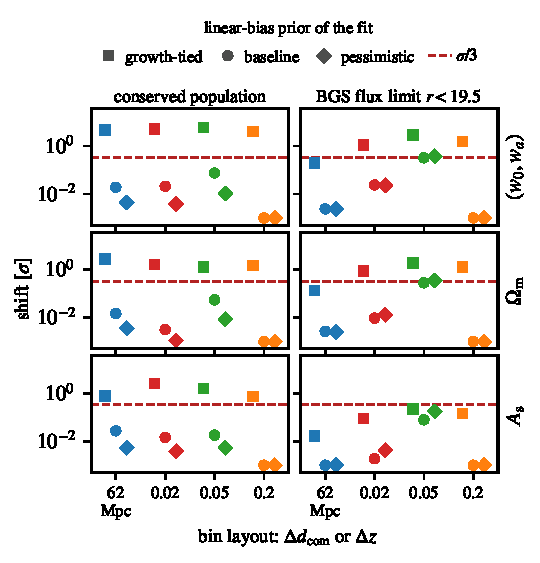
\includegraphics[width=0.62\linewidth]{plots/drift_shifts/drift_shifts.pdf}
  \caption{The shift of a model A baseline fit under each known drift
    alone: the conserved-population drift (left) and the BGS
    $r < 19.5$ flux limit (right); $(w_0, w_a)$ in units of the fit's
    ellipse, $\Omega_m$ and $A_s$ in their own $\sigma$.  Markers: the
    linear-bias prior of the fit; colors: the layouts.  Dashed line:
    $\sigma/3$.  Points on the bottom axis: values below $10^{-3}$,
    among them the exact zeros of the baseline and pessimistic priors
    on $\Delta z = 0.2$.  Omitted: the free prior, which absorbs both
    drifts exactly, and model A pessimistic.  \kmaxclause}
  \label{fig:driftshifts}
\end{figure}

\section{Numerical checks}
\label{app:checks}

\begin{itemize}
  \item \textbf{The chain rule.}  For every group, the per-bin columns
    of Eq.~\eqref{eq:chain}, summed with the weights $1/D(\bar{z}_i)$,
    reproduce the stencil derivative of the group amplitude $B_g$ to
    $9.8\times10^{-8}$, $1.2\times10^{-7}$, $4.0\times10^{-8}$ and
    $1.3\times10^{-8}$ of the stencil column's largest entry (layout
    order): the operator columns through the bias setter and the full
    likelihood through the stencil agree.
  \item \textbf{The matched-prior identity.}  When a fit's prior equals
    the truth's scatter, the identity $\Prec\Sigma\Prec = \Prec$ of
    Appendix~\ref{sec:inflation} makes the scatter and noise terms of
    $\langle\chi^2_w\rangle$ sum to exactly $2$.  Over every layout and
    variant, $\max|\langle\chi^2_w\rangle - \Delta_{\rm drift}^2 - 2|
    = 9.4\times10^{-10}$.
  \item \textbf{Exact recovery.}  The free prior must absorb any truth
    of the linear bias.  Its largest mean $(w_0, w_a)$ shift over the
    random truths is $1.9\times10^{-11}$.
  \item \textbf{One direction without information.}  On
    $\Delta d_{\rm com} = 62$~Mpc at this cut only $7$ of the $18$ BGS
    bins keep any band.  Under model A pessimistic on the free prior,
    the flat-prior BGS tilts of $\Delta_2$, $\Delta_s$ and $\alpha_0$
    then leave one combination of parameters with no information, and a
    plain matrix inverse amplified round-off along it into a spurious
    $2\sigma$ shift.  The notebook therefore scales every Fisher matrix
    to unit diagonal, diagonalizes it, and drops the directions whose
    eigenvalue is below $10^{-12}$ of the largest.  Exactly one of the
    $48$ systems (four layouts, four linear-bias priors, and three
    higher-order configurations: model A baseline, model A pessimistic
    and the exact calibrations of Appendix~\ref{app:comparison}) drops
    one direction, whose largest component on $(w_0, w_a)$, $\Omega_m$
    and $A_s$ is $6.3\times10^{-12}$: a pure nuisance combination.
  \item \textbf{The $\alpha_0$ step.}  At the negative stencil point,
    $\alpha_0 = -5\aunit$, the factor $b_1^2 + \alpha_0 k^2$ of the
    linear and counterterm pieces turns negative above
    $k \approx 0.6\hMpc$, where the low-rank engine floors
    $\sqrt{P_{gg}}$.  On $\Delta z = 0.05$, a step of $5$ against a step
    of $1$ changes the $\alpha_0$ columns by at most
    $3.5\times10^{-4}$ of each column's largest entry.
  \item \textbf{Reproducibility.}  A recomputation of the
    $\Delta z = 0.05$ derivatives is bitwise identical to the cache.
  \item \textbf{The loop templates.}  With $b_3 = 0$, CosmoLike's
    C-FAST-PT loop templates and Python FAST-PT agree on the
    $\Delta d_{\rm com} = 62$~Mpc vector, pairs included, to a
    $\Delta\chi^2$ far below one (subsection ``Gaps against model A'' of
    \texttt{notes/higher\_order\_bias}).
\end{itemize}

\section{The counterterm requires the low-rank engine}
\label{app:counterterm}

CosmoLike has two non-Limber engines for $C_\ell^{gg}$.  FKEM, the
FFTLog method of Fang et al.~\cite{FangKEM2020}, projects the linear
term exactly and moves everything nonlinear, the counterterm included,
through its Limber difference, so its one-loop content is Limber.  The
low-rank engine factorizes each bin's full one-loop $P_{gg}$, less the
white-noise constant of the loops (which Limber projects exactly), and
projects it without the Limber approximation.

For the counterterm the difference is large.  On the $\Delta z = 0.05$
layout the low-rank $\alpha_0$ response, $\partial C_\ell/\partial\alpha_0$,
is $7.3$ times the Limber one at $\ell = 20$, $1.8$ times at
$\ell = 50$, $1.26$ times at $\ell = 100$ and about $1.05$ times at
$\ell = 200$--$400$ (median over the kept auto spectra).  The reason
is the radial modes of thin bins.  Limber evaluates the power at the
transverse wavenumber $k = (\ell + 1/2)/\chi$ only.  A thin bin with
sharp edges also passes radial modes of higher $k$, and the $k^2$
weight of the counterterm amplifies them; at low $\ell$, where the
transverse wavenumber is small, they dominate the response.  The
low-rank response is converged: raising
\texttt{nonlimber\_accuracyboost} from $32$ to $128$, the rank from $5$
to $10$, or the overall accuracy boost from $1$ to $2$ changes it by a
$\Delta\chi^2$ far below one.  For a one-sigma $\alpha_0$ the two
engines' responses differ by tens of units of $\chi^2$, while at
$\alpha_0 = 0$ they agree on the full vector to a few units.  The
forecast uses the low-rank engine.

\section{Comparison with linear bias and with exact calibrations}
\label{app:comparison}

Neither comparison in this appendix is a result of this note.  The
linear-bias run uses a model that \texttt{notes/linear\_bias\_kmax}
shows is already biased at this cut, and exact calibrations assume
that $b_2$ and $\bstwo$ are known exactly.  Both sets of FoMs are in
\texttt{plots/baseline\_ladder/data.json} and in the notebook's printed
ladder table.

\paragraph{Linear bias.}
Model A baseline keeps about $88$, $93$, $74$ and $50\%$ of the
linear-bias run's ${\rm FoM}(w_0, w_a)$ on the baseline prior, and model
A pessimistic about $82$, $81$, $55$ and $30\%$ on the pessimistic prior
(layouts in the order $\Delta d_{\rm com} = 62$~Mpc, $\Delta z = 0.02$,
$0.05$, $0.2$).  The loss grows as the bins widen.  A likely reason: on
the wide layouts a group holds few bins, so one offset per group is
close to one offset per bin, and the new parameters compete with each
bin's linear bias for the same band powers.

\paragraph{Exact calibrations.}
With the calibrations taken as exact, the FoM exceeds that of the
linear-bias run under every prior and on every layout: on the baseline
prior about $1.4$ times on $\Delta d_{\rm com} = 62$~Mpc and $2.0$ times
on $\Delta z = 0.05$.  The loop terms are then not free: with $b_{2,i}$
and $b_{s^2,i}$ fixed by the calibrations at $b_{1,i}$, and
$\alpha_0 = {\rm SN}_0 = 0$, the one-loop correction is a known function
of $b_{1,i}$ and of the matter power spectrum.  The loop terms grow as
the fourth power of the growth factor and the linear term as $b_1^2$
times its square, so the size of the correction relative to the linear
term carries information on the amplitude of the matter fluctuations
that a linear-bias model does not have.  That information is only as
good as the calibrations: with exact calibrations the calibration drift
shifts $(w_0, w_a)$ by $0.8$--$1.9\sigma$ under the growth-tied prior
and by $0.06$--$0.48\sigma$ under the other three.  The offsets of
model A baseline, with widths set by the known scatter of the
calibrations, and its $\alpha_0$ and ${\rm SN}_0$ remove this
information, and model A baseline sits below the linear-bias run under
every prior and on every layout.

\section{Limitations}
\label{app:limits}

\begin{itemize}
  \item \textbf{Linear response.}  The shifts and $\chidof$ are first
    order in the truth's departure from the fiducial.  The dropped
    second-order term is a few percent of the shift for $1$--$3\%$
    residuals and perhaps $10$--$20\%$ for the $22\%$ BGS drift
    (Appendix~\ref{sec:randomtruths}).
  \item \textbf{Theory truths, not mocks.}  The project is a theory
    paper.  The truths are the derived drifts, Gaussian residuals of the
    two stated sizes, and one linear drift of the calibrations.
    Residuals rougher than the pessimistic prior, and calibrations that
    drift nonlinearly within a group, are untested.
  \item \textbf{Real-space loops.}  Model A adds the real-space one-loop
    terms to linear Kaiser distortions.
\end{itemize}

\section{Open issues}
\label{app:open}

\begin{itemize}
  \item \textbf{One-loop terms in the covariance.}  The covariance is
    Gaussian with linear bias $B_g/D(\bar{z}_i)$; it leaves out the
    one-loop terms of model A, which make up about $2\%$ of the kept
    spectra (median $1.6$--$2.3\%$ over the layouts).
  \item \textbf{The scale cut was not rebuilt on the one-loop model.}
    Applied to the $\alpha_0$ template $\partial C_\ell/\partial\alpha_0$,
    the UV fraction of Eq.~\eqref{eq:uvfraction} is a median $0.076$ and
    a maximum $0.14$ on the kept bands, all above $0.05$, against a
    median $0.017$ and a maximum $0.052$ for the fiducial model A
    vector.  Part of what the forecast learns about $\alpha_0$ therefore
    comes from scales the cut is meant to exclude.
  \item \textbf{Negative $\alpha_0$ in chains.}  The linear and
    counterterm pieces combine to $(b_1^2 + \alpha_0 k^2)\,P_{\rm mm}$,
    negative above $k \approx b_1/\sqrt{|\alpha_0|}$.  At
    $\alpha_0 = -88.9\aunit$, one prior width below zero, the spectrum
    the low-rank engine factorizes turns negative above
    $k \approx 0.14\hMpc$, the engine floors $47\%$ of its grid, and the
    vector curves in $\alpha_0$, which is harmless for the Fisher forecast
    at $\alpha_0 = 0$, but not for chains that explore negative
    $\alpha_0$.  The two remedies, a loop taper above the scale where
    one-loop perturbation theory is trusted and a positivity prior on
    $P_{gg}$ (subsection ``The white-noise limit of the renormalized
    loops'' of \texttt{notes/higher\_order\_bias}), are not
    implemented.
  \item \textbf{The $b_3$ template is broken.}  CosmoLike's third-order
    bias template is a fixed table that is wrong even at the fiducial;
    model A sets $b_3 = 0$, as in DESI's baseline, where the template
    drops out (\texttt{notes/higher\_order\_bias}).
\end{itemize}

\begin{thebibliography}{99}

\bibitem{Saraivanov2026}
E. Saraivanov, H. Rubira, V. Miranda and T. Eifler,
``Towards the Two-Loop EFTofLSS in Galaxy Lensing Surveys'',
2026, arXiv:2603.13031.

\bibitem{DeRoseChen2025}
J. DeRose and S. Chen,
``The Lensing Counter Narrative: An Effective Description of
Small-Scale Clustering in Weak Lensing Power Spectra'',
2025, arXiv:2510.18981.

\bibitem{Lazeyras2016}
T. Lazeyras, C. Wagner, T. Baldauf and F. Schmidt,
``Precision measurement of the local bias of dark matter halos'',
2016, arXiv:1511.01096.

\bibitem{Saito2014}
S. Saito, T. Baldauf, Z. Vlah, U. Seljak, T. Okumura and P. McDonald,
``Understanding higher-order nonlocal halo bias at large scales by
combining the power spectrum with the bispectrum'',
2014, arXiv:1405.1447.

\bibitem{DESI2024V}
DESI Collaboration,
``DESI 2024 V: Full-shape galaxy clustering from galaxies and
quasars'',
2024, arXiv:2411.12021.

\bibitem{Maus2024}
M. Maus, S. Chen, M. White et al.,
``An analysis of parameter compression and full-modeling techniques
with Velocileptors for DESI 2024 and beyond'',
2024, arXiv:2404.07312.

\bibitem{DESCSRD2018}
The LSST Dark Energy Science Collaboration,
``The LSST Dark Energy Science Collaboration (DESC) Science
Requirements Document'',
2018, arXiv:1809.01669.

\bibitem{FangKEM2020}
X. Fang, E. Krause, T. Eifler and N. MacCrann,
``Beyond Limber: Efficient computation of angular power spectra for
galaxy clustering and weak lensing'',
2020, JCAP, 05, 010,
arXiv:1911.11947.

\bibitem{Fry1996}
J. N. Fry,
``The Evolution of Bias'',
1996, ApJ, 461, L65.

\bibitem{TegmarkPeebles1998}
M. Tegmark and P. J. E. Peebles,
``The Time Evolution of Bias'',
1998, ApJ, 500, L79,
arXiv:astro-ph/9804067.

\bibitem{Wake2008}
D. A. Wake et al.,
``The 2dF-SDSS LRG and QSO Survey: evolution of the clustering of
luminous red galaxies since $z = 0.6$'',
2008, MNRAS, 387, 1045,
arXiv:0802.4288.

\bibitem{Tojeiro2012}
R. Tojeiro et al.,
``The progenitors of present-day massive red galaxies up to
$z \sim 0.7$: finding passive galaxies using SDSS-I/II and SDSS-III'',
2012, MNRAS, 424, 136,
arXiv:1202.6241.

\bibitem{Guo2013}
H. Guo et al.,
``The clustering of galaxies in the SDSS-III Baryon Oscillation
Spectroscopic Survey: luminosity and color dependence and redshift
evolution'',
2013, ApJ, 767, 122,
arXiv:1212.1211.

\bibitem{Zhou2021}
R. Zhou et al.,
``The clustering of DESI-like luminous red galaxies using photometric
redshifts'',
2021, MNRAS, 501, 3309,
arXiv:2001.06018.

\bibitem{Zhou2023lrg}
R. Zhou et al.,
``Target Selection and Validation of DESI Luminous Red Galaxies'',
2023, AJ, 165, 58,
arXiv:2208.08515.

\bibitem{Zhou2023tomo}
R. Zhou et al.,
``DESI luminous red galaxy samples for cross-correlations'',
2023, JCAP, 11, 097,
arXiv:2309.06443.

\bibitem{White2022}
M. White et al.,
``Cosmological constraints from the tomographic cross-correlation of
DESI luminous red galaxies and Planck CMB lensing'',
2022, JCAP, 02, 007,
arXiv:2111.09898.

\bibitem{Sailer2024}
N. Sailer et al.,
``Cosmological constraints from the cross-correlation of DESI
luminous red galaxies with CMB lensing from Planck PR4 and ACT DR6'',
2025, JCAP, 06, 008,
arXiv:2407.04607.

\bibitem{Sailer2025}
N. Sailer et al.,
``Evolution of structure growth during dark energy domination:
insights from the cross-correlation of DESI galaxies with CMB lensing
and galaxy magnification'',
2025, Phys. Rev. D,
arXiv:2503.24385.

\bibitem{Zehavi2011}
I. Zehavi et al.,
``Galaxy Clustering in the Completed SDSS Redshift Survey: The
Dependence on Color and Luminosity'',
2011, ApJ, 736, 59,
arXiv:1005.2413.

\bibitem{Blanton2003}
M. R. Blanton et al.,
``The Galaxy Luminosity Function and Luminosity Density at Redshift
$z = 0.1$'',
2003, ApJ, 592, 819,
arXiv:astro-ph/0210215.

\bibitem{BlantonRoweis2007}
M. R. Blanton and S. Roweis,
``K-corrections and Filter Transformations in the Ultraviolet,
Optical, and Near-Infrared'',
2007, AJ, 133, 734,
arXiv:astro-ph/0606170.

\bibitem{Hahn2023}
C. Hahn et al.,
``The DESI Bright Galaxy Survey: Final Target Selection, Design, and
Validation'',
2023, AJ, 165, 253,
arXiv:2208.08512.

\bibitem{Raichoor2023}
A. Raichoor et al.,
``Target Selection and Validation of DESI Emission Line Galaxies'',
2023, AJ, 165, 126,
arXiv:2208.08513.

\bibitem{Rocher2023}
A. Rocher et al.,
``The DESI One-Percent Survey: exploring the halo occupation
distribution of emission line galaxies with AbacusSummit
simulations'',
2023, JCAP, 10, 016,
arXiv:2306.06319.

\end{thebibliography}

\end{document}
